\documentclass[12pt]{report}
\usepackage{setspace}
%\linespread{1.1}
\linespread{1.6}
%\spacing{1.45}
\usepackage{indentfirst}
\usepackage{graphicx}
\graphicspath{ {./lateximages} }
\usepackage{float}
\usepackage{amsmath}
\usepackage{newtxtext}
\usepackage{newtxmath}
\usepackage{geometry}
\geometry{
 a4paper,
 left=4cm,
 top=4cm,
 bottom=3cm,
 right=3cm
 }
\usepackage{tocloft}
\usepackage{multicol}
\usepackage{Tabbing}
\usepackage{array}
\usepackage{multirow}
\usepackage{longtable}
\usepackage{pdfpages}
\usepackage{caption}
\usepackage{fancyhdr}

%bikin item di table center secara vertical
%\renewcommand\tabularxcolumn[1]{m{#1}}


\usepackage{titlesec}
\titleformat{\section}{\normalfont\normalsize\bfseries\centering}{}{0pt}{}
\titleformat*{\subsection}{\normalfont\normalsize\bfseries}


\usepackage[hidelinks]{hyperref}
\usepackage[all]{hypcap}

\makeatletter
\counterwithin{figure}{section}
%\renewcommand{\fnum@figure}{Gambar \thefigure}
\renewcommand{\fnum@figure}{\thefigure}
\renewcommand{\thefigure}{\arabic{section}.\arabic{figure}}
\makeatother

\makeatletter
\counterwithin{table}{section}
%\renewcommand{\fnum@table}{Tabel \thetable}
\renewcommand{\fnum@table}{\thetable}
\renewcommand{\thetable}{\arabic{section}.\arabic{table}}
\makeatother


\setcounter{tocdepth}{3}
\setcounter{secnumdepth}{3}

\setlength{\cftfignumwidth}{70pt}
\setlength{\cfttabnumwidth}{70pt}
\setlength{\cftsecnumwidth}{50pt}
\setlength{\cftsubsecnumwidth}{20pt}
\setlength{\cftsubsecindent}{70pt}
%\renewcommand{\cftsecfont}{\bfseries}
\setlength{\cftsubsubsecindent}{90pt}
\setlength{\cftsubsubsecnumwidth}{20pt}
\def\seqinsert{\-}

\usepackage[sectionbib]{apacite}
\usepackage[english]{babel}
\addto{\captionsenglish}{\renewcommand{\refname}{DAFTAR PUSTAKA}}
\tolerance=1
\emergencystretch=\maxdimen
\hyphenpenalty=10000
\hbadness=10000

\begin{document}

\begin{titlepage}
	\begin{center}
	\singlespacing
	\vspace*{1cm}
	\textbf{\fontsize{16pt}{\baselineskip}\selectfont
		RANCANG BANGUN SISTEM PENCARIAN TEKS DENGAN MENGGUNAKAN MODEL \textit{CONTINUOUS-BAG-OF-WORDS} DAN MODEL \textit{CONTINUOUS SKIP-GRAM} PADA KOLEKSI DOKUMEN}

	\vspace{1.8cm}
	\textbf{\fontsize{14pt}{\baselineskip}\selectfont 
		Skripsi}
        
	\vspace{1.8cm}
	\textbf{\fontsize{14pt}{\baselineskip}\selectfont
		Disusun untuk memenuhi salah satu syarat \\memperoleh gelar Sarjana Komputer}
            
	\vspace{1.8cm}

       	
\includegraphics[width=3cm]{logounj}

	\vspace{1.5cm}
            
	\textbf{\fontsize{14pt}{\baselineskip}\selectfont
		Muhammad Zalghornain \\ 3145153000}
            
	\vspace{2.5cm}
     
	\textbf{\fontsize{13pt}{\baselineskip}\selectfont
	PROGRAM STUDI ILMU KOMPUTER\\
	FAKULTAS MATEMATIKA DAN ILMU PENGETAHUAN ALAM\\
	UNIVERSITAS NEGERI JAKARTA}
            
	\vspace{0.8cm}
	\textbf{\fontsize{12pt}{\baselineskip}\selectfont
	2023}
	
	\end{center}
\end{titlepage}

\pagenumbering{roman}

\cleardoublepage
\phantomsection

\addcontentsline{toc}{section}{LEMBAR PERSETUJUAN HASIL SIDANG SKRIPSI}
%\section*{LEMBAR PERSETUJUAN HASIL SIDANG SKRIPSI}
\includepdf[pages={1}]{lembar_persetujuan_hasil_sidang_skripsi_lengkap.pdf}
%\includepdf[pages={1}]{lembar_pengesahan.pdf}

%Dengan ini saya mahasiswa Fakultas Matematika dan Ilmu Pengetahuan Alam, Universitas Negeri Jakarta
%\begin{tabbing}
%\hspace{18pt}\= Nama\hspace{30mm}\=:  Muhammad Zalghornain \\  
%\> No. Registrasi\>:   3145153000 \\
%\> Program Studi\>:  Ilmu Komputer \\
%\> Judul\> : Rancang Bangun Sistem Pencarian Teks Dengan \\
%\> \> Menggunakan Model \textit{Continuous-Bag-Of-Words} Dan \\
%\> \> Model \textit{Continuous Skip-Gram} Pada Koleksi Dokumen
%\end{tabbing}
%Menyatakan bahwa proposal skripsi ini telah siap diajukan untuk seminar pra skripsi. 


%\begin{center}
%    Menyetujui:
%\end{center}

%\begin{center}
%\begin{tabular}{ c m{1.7cm} c}
% Dosen Pembimbing I && Dosen Pembimbing II  \\
%\includegraphics[width=3cm]{ttd_bu_ria.png}&& \includegraphics{ttd_pak_eka.png}\\
% \textbf{\underline{Ria Arafiyah, M.Si}} && \textbf{\underline{Muhammad Eka Suryana, M.Kom}} \\  
% NIP. 19751121 200501 2 004 && NIP. 19851223 201212 1 002   
%\end{tabular}
%\end{center}

%\vspace*{0.5cm} 

%\begin{center}
%Mengetahui,\\
%Koordinator Program Studi Ilmu Komputer 


%\vspace*{3cm}


%\textbf{\underline{Ir. Fariani Hermin M.T}}\\
%NIP. 19600211 198703 2 001
%\end{center}

\linespread{1.1}\selectfont
\cleardoublepage
\phantomsection
%\section*{LEMBAR PERNYATAAN}
\addcontentsline{toc}{section}{LEMBAR PERNYATAAN}
\includepdf[pages={1}]{lembar_pernyataan_orisinalitas.pdf}

%\hfill \break
%Saya menyatakan dengan sesungguhnya bahwa skripsi dengan judul "\textbf{Rancang Bangun Sistem Pencarian Teks dengan Menggunakan Model \textit{Continuous-Bag-of-Words} dan Model \textit{Continuous Skip-Gram} pada Koleksi Dokumen}" yang disusun sebagai syarat untuk memperoleh gelar Sarjana Komputer dari Program Studi Ilmu Komputer Universitas Negeri Jakarta adalah karya ilmiah saya dengan arahan dari dosen pembimbing.
%\newline

%Sumber informasi yang diperoleh dari penulis lain yang telah dipublikasikan yang disebutkan dalam teks skripsi ini, telah dicantumkan dalam Daftar Pustaka sesuai dengan norma, kaidah dan etika penulisan ilmiah.
%\newline

%Jika di kemudian hari ditemukan sebagian besar skripsi ini bukan hasil karya saya sendiri dalam bagian-bagian tertentu, saya bersedia menerima sanksi pencabutan gelar akademik yang saya sanding dan sanksi-sanksi lainnya sesuai dengan peraturan perundang-undangan yang berlaku.
%\newline

%\begin{center}
%\begin{tabular}{ m{9cm} c}
%& Jakarta, 28 Februari 2023 \\
%& \\
%& \\
%& \\
%& \\
%& \\
%& Muhammad Zalghornain \\   
%\end{tabular}
%\end{center}



\linespread{1.6}\selectfont
\cleardoublepage
\phantomsection
\section*{KATA PENGANTAR}
\addcontentsline{toc}{section}{KATA PENGANTAR}

Segala puji dan syukur kepada Allah Subhanahu wa ta’ala, karena telah memberikan berkah dan rahmat-Nya sehingga penulis dapat menyelesaikan penyusunan tugas akhir ini dengan judul “Rancang Bangun Sistem Pencarian Teks dengan Menggunakan Model \textit{Continuous-Bag-of-Words} dan Model \textit{Continuous Skip-Gram} pada Koleksi Dokumen”. Keberhasilan dalam menyusun dan menyelesaikan tugas akhir ini tidak lepas dari bantuan berbagai pihak yang memberikan dukungan moril dan materil. Oleh karena itu, pada kesempatan ini dengan kerendahan hati penulis ingin mengucapkan terima kasih kepada:
\begin{enumerate}
\item Ibu Ir. Fariani Hermin Indiyah, M.T selaku Koordinator Program Studi Ilmu Komputer yang selalu mendorong mahasiswa untuk menyelesaikan Tugas Akhir.
\item Ibu Ria Arafiyah, M.Si selaku dosen pembimbing I yang telah membimbing, mengarahkan, serta memberikan saran yang baik untuk penulis dalam menyelesaikan Tugas Akhir ini.
\item Bapak Muhammad Eka Suryana, M.Kom. selaku dosen pembimbing II yang telah membimbing, mengarahkan, serta memberikan saran yang baik untuk penulis dalam menyelesaikan Tugas Akhir ini.
\item Bapak Med Irzal, M.Kom., selaku dosen pembimbing akademis penulis yang senantiasa membantu mahasiswa.
\item Para dosen dan teman-teman Program Studi Ilmu Komputer angkatan 2015 yang selalu membantu dan mendukung sehingga Tugas Akhir ini dapat diselesaikan dengan baik.
\item Kedua orang tua dan kakak penulis yang senantiasa memberikan dukungan untuk menyelesaikan Tugas Akhir.
\end{enumerate}
Penulis menyadari bahwa tugas akhir ini masih jauh dari kata sempurna, oleh karena itu, Penulis dengan senang hati menerima kritik dan saran yang bersifat membangun dari semua pihak sehingga tugas akhir ini dapat disusun menjadi lebih baik lagi.
Akhir kata harapan Penulis agar tugas akhir ini dapat berguna sebagai sumber bacaan bagi seluruh kalangan sehingga dapat bermanfaat bagi lingkungan akademik maupun pihak lain yang membutuhkannya. Atas perhatiannya, Penulis mengucapkan terima kasih.

\vspace*{0.5cm}
\begin{flushright}
Jakarta, 6 Februari 2023
\vspace*{1cm}

Penulis
\end{flushright}

\linespread{1.1}\selectfont

\cleardoublepage
\phantomsection
\section*{ABSTRAK}
\addcontentsline{toc}{section}{ABSTRAK}
\hfill \break
{\parindent0pt
\textbf{MUHAMMAD ZALGHORNAIN. Rancang Bangun Sistem Pencarian Teks dengan Menggunakan Model \textit{Continuous-Bag-of-Words} dan Model \textit{Continuous Skip-Gram} pada Koleksi Dokumen. Skripsi. Fakultas Matematika dan Ilmu Pengetahuan Alam, Universitas Negeri Jakarta. 2023. Di bawah bimbingan Ria Arafiyah, M.Si dan Muhammad Eka Suryana, M.Kom.}
\newline

Dengan banyaknya data yang dibutuhkan, diperlukan suatu alat untuk mensortir data yang diinginkan secara cepat dan mudah. \textit{Search engine} merupakan salah satu cara untuk mensortir data sesuai keinginan yang dibutuhkan \textit{user} berdasarkan kata yang di-\textit{input user} secara cepat dan mudah. Sistem \textit{search engine} tradisional hanya menggunakan jumlah frekuensi kata pada dokumen untuk mencari kata yang relevan. Diperlukan cara untuk mengerti kueri \textit{user} agar bisa didapatkan hasil pencarian yang sesuai keinginan \textit{user} terlepas keterbatasan kueri \textit{user}. Akan digunakan metode \textit{Continuous-Bag-of-Words} dan \textit{Continuous Skip-Gram} untuk mencari kata di sekitar kata yang di-\textit{input user} yang lalu akan digunakan untuk melakukan pencarian dokumen. Hasil menunjukkan bahwa \textit{neutral network} tidak cocok digunakan untuk mesin pencarian karena waktu \textit{training}-nya yang lama untuk mendapatkan hasil yang diinginkan. Sedangkan untuk hasil relevansinya, metode \textit{Continuous-Bag-of-Words} dapat menghasilkan hasil relevan dengan hasil kesesuaian 86.67\% terhadap hasil \textit{ranking} \textit{user}.
\newline

\textbf{Kata kunci} : \textit{Continuous-Bag-of-Words}, \textit{Continuous-Skip-Gram},  pencarian, pencarian teks, \textit{ranking} dokumen, relevansi dokumen.
}


\cleardoublepage
\phantomsection
\section*{ABSTRACT}
\addcontentsline{toc}{section}{ABSTRACT}
\hfill \break
{\parindent0pt
\textbf{MUHAMMAD ZALGHORNAIN. Building a Text Search System using Continuous-Bag-of-Words Model and Continuous Skip-Gram Model on a Collection of Documents. Thesis. Faculty of Mathematics and Natural Sciences, State University of Jakarta. 2023. Supervised by Ria Arafiyah, M.Si and Muhammad Eka Suryana, M.Kom.}
\newline

With so much data that is needed, there is a need for some tools to sort all the data that we want quickly and easy. Search engine is one of the tools that is used to sort data quickly and easy that the user want according to the words that he input in. Traditional search engine system usually only used words frequency on the document to find the relevant document. There is a need to understand users query so users could get result they want regardless of users query limitations. Continuous-Bag-of-Words models and Continuous Skip-Gram models will be used to search for the words around the words that user input to search for the document. The results shows that neural network isn't exactly good to be used for search engine because of it's training time that could take a while to get a good results. As for the relevancy, Continuous-Bag-of-Words models can get a relevant results with accuracy of 86.67\% compared to user ranking results.
\newline

\textbf{Keywords} : \textit{Continuous-Bag-of-Words, Continuous-Skip-Gram, document ranking, document relevancy, searching, text searching.}
}
\linespread{1.6}


\cleardoublepage
\phantomsection
\setlength{\cftbeforetoctitleskip}{0pt}
\setlength{\cftaftertoctitleskip}{20pt}
\addcontentsline{toc}{section}{DAFTAR ISI}
\renewcommand{\contentsname}{\hfill\bfseries\normalsize DAFTAR ISI \hfill}   
\renewcommand{\cftaftertoctitle}{\hfill}
\renewcommand{\listfigurename}{\hfill\bfseries\normalsize DAFTAR GAMBAR}
\renewcommand{\cftafterloftitle}{\hfill}
\renewcommand{\listtablename}{\hfill\bfseries\normalsize DAFTAR TABEL \hfill}
\renewcommand{\cftafterloftitle}{\hfill}
\tableofcontents


\cleardoublepage
\phantomsection
\setlength{\cftbeforeloftitleskip}{0pt}
\setlength{\cftafterloftitleskip}{20pt}
\addcontentsline{toc}{section}{DAFTAR GAMBAR}
\listoffigures


\cleardoublepage
\phantomsection
\setlength{\cftbeforelottitleskip}{0pt}
\setlength{\cftafterlottitleskip}{20pt}
\addcontentsline{toc}{section}{DAFTAR TABEL}
\listoftables



\linespread{1.6}\selectfont

\renewcommand\thefigure{\normalsize Gambar \arabic{section}.\arabic{figure} :}
\renewcommand\thetable{\normalsize Tabel \arabic{section}.\arabic{table} :}
\renewcommand\thesection{\normalsize BAB \Roman{section}}
\renewcommand\thesubsection{\normalsize  \Alph{subsection}.}
\renewcommand\thesubsubsection{\normalsize  \arabic{subsubsection}.}

\captionsetup[figure]{labelsep=space}
\captionsetup[table]{labelsep=space}

\setlength{\LTpre}{0pt}
\setlength{\LTpost}{0pt}

\newpage
\pagestyle{fancy}
\fancyhead{}
\fancyhead[CF]{}
\fancyhead[LH]{}
\fancyhead[RH]{\thepage}
\renewcommand{\headrulewidth}{0pt}
\pagenumbering{arabic}
\section[PENDAHULUAN]{BAB I}
\section*{PENDAHULUAN}
\thispagestyle{plain}

\subsection{Latar Belakang}
Web merupakan tempat penyimpanan informasi dalam bentuk teks, gambar, audio dan video. Dengan banyaknya informasi yang ada di web, diperlukan alat untuk mencari dan mendapatkan sesuatu yang diperlukan pengguna dengan mudah.

\textit{Web Search Engine} merupakan sistem perangkat lunak yang di desain untuk melakukan pencarian. Definisi dasar \textit{search engine} bisa merujuk pada sistem \textit{Information Retrieval} (IR) yang memungkinkan pencarian ``kata kunci'' pada teks digital terdistribusi \cite{halavais2017search}. \textit{Search engine} melakukan pencarian pada sistem dengan sistematik untuk menemukan informasi spesifik yang di \textit{input}. Hasil pencarian biasanya di tampilkan dalam bentuk \textit{list}. Infomasi yang ditampilkan bisa campuran dari \textit{link} ke halaman web, gambar, video, artikel, paper, dan hal lainnya. Beberapa \textit{search engine} juga melakukan pencarian pada database dan direktori terbuka. Tidak seperti web direktori yang perlu di tangani oleh manusia, \textit{search engine} juga bisa menjaga informasi selalu \textit{real-time} dengan menggunakan algoritma pada \textit{web crawler}. \textit{Web search engine} merupakan salah satu contoh pengaplikasian \textit{Information Retrieval} atau Sistem Temu Balik Informasi.

\textit{Information Retrieval} (IR) merupakan pencarian material (biasanya dokumen) tak berstruktur (biasanya teks) yang memenuhi kebutuhan informasi dari koleksi besar (biasanya disimpan di komputer) \shortcite{manning2010introduction}. IR dibutuhkan untuk mensortir data yang relevan secara otomatis terhadap \textit{input} yang dimasukkan \textit{user}, sehingga \textit{user} tidak perlu mensortir data sendiri, terutama jika data tersebut ada dalam jumlah yang besar.

Pe-\textit{ranking}-an merupakan hal yang penting dalam \textit{Information Retrieval}, mengembalikan dokumen yang diinginkan \textit{user} merupakan bagian yang penting dalam \textit{search engine}. Sistem pencarian tradisional biasanya menggunakan jumlah frekuensi kata pada dokumen untuk mencari dokumen yang relevan terhadap kueri \textit{user}. Walaupun metode ini tidak membutuhkan biaya komputasi yang tinggi, model ini memiliki kelemahan pada keterbatasan kata. Ketika pencari tidak mengetahui istilah tepat untuk suatu konsep, akan cukup sulit bagi pencari untuk mendapatkan informasi yang ia inginkan. Maka dari itu dibutuhkan suatu cara untuk mengerti kueri \textit{user}, untuk mengerti apa yang \textit{user} ingin cari terlepas keterbatasan kueri yang dimasukkan \textit{user}.

\textit{Query Expansion} merupakan teknik yang biasa di gunakan pada \textit{Information Retrieval} untuk meningkatkan performa pengambilan data dengan memodifikasi kueri original, dengan menambahkan kata baru atau pembobotan ulang kata original. Menurut \citeA{doi:10.1177/0165551506065787}, ``\textit{Query Expansion} idealnya harus memiliki beberapa karakteristik, salah satunya merupakan hubungan semantik dengan kueri original''. Penimbangan semantik kata bertujuan untuk mengerti maksud \textit{user} untuk menghasilkan hasil pencarian yang lebih relevan. Dengan mempertimbangkan makna semantik diharapkan dapat meningkatkan kualitas pencarian dan mengurangi waktu \textit{user} untuk memilah-milah dokumen yang relevan. Pada penelitiannya yang berjudul ``\textit{Enhanced word embedding similarity measures using fuzzy rules for query expansion}'', \shortciteA{8015482} menemukan bahwa \textit{Query Expansion} menggunakan \textit{Word Embedding} dapat meningkatkan performa pe-\textit{ranking}-an dokumen dibanding metode tradisional.

\textit{Word Embedding} merupakan representasi kata-kata dalam bentuk vektor, dimana kata yang mirip akan berdekatan pada ruang vektor. \textit{Word Embedding} dapat menangkap makna semantik dari kata. Salah satu cara untuk menghasilkan \textit{Word Embedding} merupakan \textit{Word2vec}. Menurut \citeA{10.1145/3388218.3388229}, \textit{Word2vec} merupakan salah satu model paling umum yang digunakan dalam \textit{Word Embedding}. \textit{Word2vec} menggunakan \textit{neural network} yang terdiri dari dua model yaitu \textit{Continuous Bag-of-Words} atau CBOW dan \textit{Continuous Skip-Gram} atau \textit{Skip-Gram}. CBOW menggunakan kata konteks (kata di sekitar kata target) untuk memprediksi kata target, sedangkan \textit{Skip-Gram} menggunakan kata target untuk memprediksi kata di sekitarnya atau kata konteks. Pada penelitiannya, \shortciteA{word2vec} menemukan bahwa CBOW memiliki hasil akurasi sintaksis lebih tinggi daripada \textit{Skip-Gram} terhadap kata yang sering muncul, sedangkan Skip-Gram memiliki akurasi semantik yang lebih tinggi dibanding CBOW. Pendekatan \textit{Word2vec} telah banyak digunakan di berbagai eksperimen dan menjadi pijakan dalam meningkatkan ketertarikan pada \textit{Word Embedding} sebagai teknologi.

Proses pencarian pada \textit{search engine} terdiri dari \textit{crawling}, \textit{indexing}, dan \textit{searching}. Pada penelitian kali ini peneliti akan fokus terhadap bagian \textit{searching}, yaitu mengimplementasikan model \textit{Continuous Bag-of-Words} (CBOW) dan \textit{Continuous Skip-Gram} (\textit{Skip-Gram}) pada sistem pencarian teks. 

Peneiltian akan dimulai dengan pengumpulan data. Data yang dikumpulkan akan digunakan untuk melatih sistem dan juga sebagai target pencarian sistem. Sistem akan dilatih untuk menghasilkan data kata relevan dengan model CBOW dan \textit{Skip-Gram}. Setelah sistem selesai di latih, \textit{user} akan melakukan pencarian dokumen pada sistem. \textit{User} akan memasukkan \textit{keyword} pada mesin pencarian. Sistem akan mencari kata terdekat dari \textit{input} kata \textit{user} dengan menggunakan model CBOW dan \textit{Skip-Gram}. Sistem menggunakan gabungan kata relevan dan kata \textit{input} \textit{user} untuk mencari dokumen. Dokumen dengan jumlah kemunculan kata \textit{input} dan kata relevan yang tinggi akan dikeluarkan oleh sistem. Lalu di akhir \textit{user} akan menilai relevansi dokumen.

Penelitian ini merupakan bagian dari penelitian besar \textit{Search Engine}, hasil \textit{ranking} dokumen yang di dapat dari penelitian ini merupakan hasil sementara yang pada akhirnya akan digabungkan dengan metode-metode lain untuk mendapatkan hasil \textit{ranking} dokumen yang lebih baik lagi.

\subsection{Perumusan Masalah}
Berdasarkan latar belakang masalah di atas, maka dapat dirumuskan:
\begin{enumerate}
\item Bagaimana cara merancang sistem pencarian teks dengan metode \textit{Continuous-Bag-of-Words} dan \textit{Continuous Skip-Gram} ?
\item Apakah pencarian teks dengan menggunakan \textit{Continuous-Bag-of-Words} dan \textit{Continous Skip-Gram} dapat menghasilkan hasil pencarian yang relevan ?
\end{enumerate}

\subsection{Pembatasan Masalah}
Karena keterbatasan waktu, dana, tenaga, teori dan agar penelitian dapat dilakukan lebih mendalam, maka tidak semua masalah akan diteliti. Berikut merupakan batasan-batasan yang diterapkan oleh penulis:
\begin{enumerate}
\item Menggunakan kumpulan artikel yang di \textit{crawl} dari situs \textit{https://www.indosport.com}.
\item Teks yang digunakan merupakan teks bertema olahraga.
\item \textit{Tester} hanya menilai hasil lima dokumen teratas yang dikeluarkan sistem.
\end{enumerate}

\subsection{Tujuan Penelitian}
Berdasarkan perumusan masalah di atas, adapun yang menjadi tujuan dari pembuatan skripsi ini adalah :
\begin{enumerate}
\item Merancang sistem pencarian teks dengan metode CBOW dan \textit{Skip-Gram}.
\item Memvalidasi sistem pencarian.
\end{enumerate}


\subsection{Manfaat Penelitian}
Penelitian ini diharapkan dapat memberikan manfaat, antara lain:
\begin{enumerate}
\item Bagi penulis, dapat menambah pengetahuan teoritis dan praktikal penulis dalam pengembangan sistem pencarian teks.
\item Bagi Universitas Negeri Jakarta, penelitian ini diharapkan dapat menjadi acuan bagi pengembangan sistem pencarian teks yang serupa.
\item Bagi masyarakat, sebagai acuan pengetahuan metode terhadap sistem pencarian teks.
\end{enumerate}


\newpage
\section[KAJIAN PUSTAKA]{BAB II}
\section*{KAJIAN PUSTAKA}
\thispagestyle{plain}
Pada bab ini akan di jelaskan hal-hal yang berkaitan dengan penelitian yang akan dijalankan.

\subsection{\textit{Natural Language Processing}}
\textit{Natural Language Processing} (NLP) merupakan cabang dari komputer sains yang membahas tentang kemampuan komputer untuk mengerti teks dan kalimat sama seperti manusia menginterpretasikannya.

NLP menggabungkan \textit{computational linguistics} dengan statistik, \textit{machine learning}, dan \textit{deep learning model}. Teknologi-teknologi tersebut memungkinkan komputer untuk memproses bahasa manusia dalam bentuk teks atau suara dan untuk mengerti maksudnya, lengkap dengan niat dan sentimen pembicara atau penulis.

NLP banyak digunakan di aplikasi \textit{real-world} modern, cotohnya \textit{Spam detection}, \textit{Machine Translation}, \textit{Chatbot}, dan \textit{Sentiment Analysis} Media Sosial.

%\section{Log-Linear Model}

\subsection{\textit{Neural Network}}
\textit{Neural Network} merupakan kumpulan algoritma yang menyerupai otak manusia. \textit{Neural network} terdiri dari {node layers}, yang terdiri dari \textit{input}, satu atau lebih \textit{hidden layer}, dan \textit{output layer}. Setiap \textit{node} tersambung satu sama lain dan memiliki \textit{weight} diantaranya. \textit{Neural network} bergantung pada \textit{training} data untuk memperbaiki akurasi \textit{neural network} itu sendiri, tetapi setelah \textit{training}, \textit{Neural Network} dapat digunakan untuk mengklasifikasi dan mengkategorikan data dengan kecepatan tinggi. 

\textit{Neural network} terdiri dari beberapa kelas:
\begin{enumerate}
\item \textit{Feedforward Neural Network}


\textit{Feedforward Neural Network} merupakan \textit{neural network} paling sederhana. \textit{Feedforward Neural Network} hanya bergerak dalam satu arah melalui \textit{input}, \textit{hidden layer}, dan \textit{output}. Salah satu algoritma yang paling banyak digunakan untuk melatih data \textit{Feedforward Neural Network} adalah \textit{backpropagation}.


{\bfseries\textit{Backpropagation}}. \textit{Backpropagation} merupakan algoritma yang banyak digunakan untuk melatih \textit{Feedforward Neural Network}. Dalam pelatihan data, \textit{backpropagation} menghitung \textit{gradient} dari \textit{loss function} berdasarkan \textit{weight} dari \textit{neural network}, sehingga \textit{weight} bisa di ubah untuk meminimalisasi \textit{loss}.

\item \textit{Convolutional Neural Network}


\textit{Neural network} ini mirip dengan \textit{feedforward}, tapi biasanya digunakan untuk \textit{image recognition} dan \textit{pattern recognition}. Dalam \textit{neural network} ini, \textit{hidden layer} terdiri dari \textit{layer} yang melakukan konvolusi.

\item \textit{Recurrent Neural Network} (RNN)


\textit{Recurrent Neural Network} merupakan tipe \textit{neural network} yang menggunakan data sekuensial. \textit{Neural network} ini biasa digunakan untuk terjemahan, \textit{Natural Language Processing} (NLP), dan \textit{speech recognition}. Jika neural network sederhana menganggap \textit{input} dan \textit{output} independen, RNN memiliki \textit{output} yang bergantung pada elemen sebelumnya dalam sekuens.
\end{enumerate}

\subsection{\textit{Query Expansion}}
\textit{Query Expansion} merupakan proses menimbang ulang kueri untuk memperbaiki performa dalam \textit{Information Retrieval}, terutama dalam konteks pemahaman kueri. Dalam \textit{search engine}, \textit{Query Expansion} melakukan evaluasi ulang terhadap \textit{input user} dan memperbesar jangkau kueri pencarian untuk menghasilkan dokumen yang lebih banyak. Dengan menampilkan dokumen yang lebih banyak diharapkan dokumen yang tidak akan muncul pada hasil, yang memiliki kemungkinan lebih relevan terhadap kueri \textit{user}, akan masuk dalam hasil pencarian, walaupun relevan atau tidak.


\subsection{\textit{Word Embedding}}
\textit{Word Embedding} merupakan pendekatan dalam NLP (\textit{Natural Language Processing}), yang digunakan untuk merepresentasikan kata dan dokumen dalam bidang vektor. \textit{Word Embedding} didasarkan pada \textit{Distributional Hypothesis} yang mengatakan bahwa kata-kata dicirikan oleh kata-kata di sekitarnya dan kata yang sering muncul dalam konteks yang sama biasanya memiliki maksud yang mirip. Pendekatan ini  telah banyak di adoptasi oleh berbagai peneliti setelah kemajuan pada tahun 2010 terjadi tentang teoritikal kerja kualitas vektor, kemajuan kecepatan \textit{training} model, dan kemajuan \textit{hardware} memperbolehkan parameter yang lebih besar di jelajah dengan menguntungkan. Tahun 2013, \shortciteauthor{word2vec} membuat \textit{word2vec}, alat \textit{Word Embedding} yang dapat melatih teks dalam bidang vektor dengan lebih cepat dari pendekatan sebelumnya.


\subsection{Representasi kata dalam bentuk vektor}

Salah satu model yang paling populer untuk merepresentasikan kata dalam bentuk vektor adalah \textit{Feedforward Neural Net Language Model} \shortcite{aneuralprob}. Model ini terdiri dari \textit{input}, \textit{projection}, \textit{hidden layer}, dan \textit{output layer}. Model ini menjadi kompleks pada perhitungan antara \textit{projection} dan \textit{hidden layer}, karena nilai pada \textit{projection layer}-nya banyak. Untuk mengatasi keterbatasan \textit{Feedforward} NNLM, \shortciteA{RNNLM}, mengajukan RNNLM (\textit{Recurrent Neural Net Language Model}). Model ini tidak memiliki \textit{projection layer}, hanya \textit{input}, \textit{hidden} dan \textit{output}. Yang membuat model ini spesial merupakan matriks \textit{recurrent} yang menyambungkan \textit{hidden layer} dengan dirinya sendiri, yang dibatasi jangka waktu tertentu. Hal ini memungkinkan model ini membuat semacam \textit{short term memory}, informasi dari waktu sebelumnya dapat direpresentasikan dengan \textit{hidden layer} yang ter-\textit{update} berdasarkan \textit{input} sekarang dan \textit{hidden layer} di waktu sebelumnya. 



\subsection{\textit{Word2Vec}}
\shortciteA{word2vec}, mengajukan dua model baru untuk mempelajari representasi distribusi kata dengan fokus meminimalisasi kompleksitas komputasi. Dari model model sebelumnya, kompleksitas disebabkan oleh \textit{hidden layer} yang tidak linear di model model tersebut. Walaupun ini yang membuat \textit{neural network} menarik, Mikolov memilih untuk menjelajahi model yang lebih sederhana yang mungkin tidak dapat merepresentasikan data seakurat \textit{neural network} tetapi dapat di latih dengan lebih efisien.
\begin{enumerate}
\item \textit{Continuous Bag-of-Words}


Arsitektur pertama yang diajukan mirip dengan \textit{Feedforward} NNLM, dimana non-linear \textit{hidden layer}-nya dihilangkan dan \textit{projection layer}-nya digunakan oleh semua kata (bukan hanya \textit{projection} matriks-nya saja), jadi semua kata terprojeksi ke posisi yang sama (vektornya di rata-ratakan). Arsitektur ini disebut \textit{bag-of-words} model karena urutan kata sebelumnya tidak mempengaruhi projeksi. Arsitektur ini juga menggunakan kata dari setelahnya. Arsitektur ini memprediksi kata target dengan menggunakan kata konteks di sekitarnya. Berikut akan dijelaskan proses dari model CBOW yang dipaparkan oleh \shortciteA{https://doi.org/10.48550/arxiv.1411.2738}.


\begin{figure}[H]
\centering
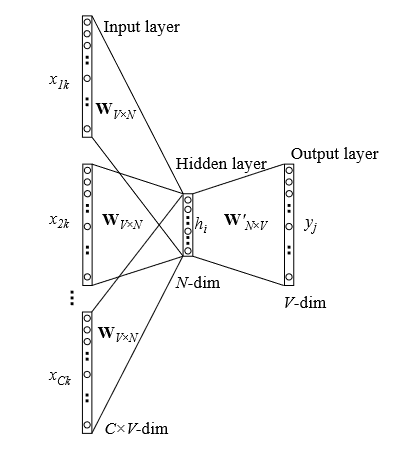
\includegraphics[scale=0.75]{modelcbow}
\caption{Model CBOW}
\label{modelcbow}
\end{figure}

Dalam gambar 1, $V$ menunjukkan ukuran kosakata, dan $N$ menunjukkan ukuran \textit{hidden layer}. \textit{Input} merupakan vektor \textit{one-hot encoded}, yang berarti untuk kata konteks masukan yang diberikan, hanya satu dari $V$ unit, ${x_1, ..., x_V }$, merupakan 1 dan unit lain merupakan 0. Contohnya dalam kalimat "budi sedang belajar matematika", \textit{one-hot encoded} dari kata “sedang” merupakan \{0 1 0 0\}.

\textit{Weight} diantara \textit{input layer} dan \textit{output layer} direpresentasikan dengan $V$x$N$ matriks $W$. Untuk mendapatkan \textit{output} pada \textit{hidden layer}, model CBOW mengambil rata-rata vektor dari kata \textit{input} konteks dan mengalikannya dengan \textit{weight matrix input}-$>$\textit{hidden}.

\begin{eqnarray}
h & = & \frac{1}{C}W^T ( X_1 + X_2 + ... + X_C)\\
& = & \frac{1}{C} ( V_{w_1} +V_{w_2}+ ... + V_{w_C})^T \label{eq2}
\end{eqnarray}

dimana $h$ merupakan \textit{hidden layer}.\\ C merupakan jumlah kata konteks.\\ $w_1, ..., w_C$ merupakan kata di konteks. \\$Vw$ merupakan vektor \textit{input} dari kata $w$. \\
Dari \textit{hidden layer} ke \textit{output layer}, ada \textit{weight matrix} berbeda, $W'$. Dengan \textit{weight} tersebut kita bisa mendapatkan $u_j$

\begin{eqnarray}
u_j = {V'_{w_j}}^Th \label{eq3}
\end{eqnarray}

$V'_{w_j}$ merupakan kolom ke $j$ dari matriks $W'$. \\Lalu kita menggunakan \textit{softmax} untuk mendapatkan distribusi posterior kata.

\begin{equation}
p(w_j|w_I) = y_j = \frac {\text{exp}(u_j)}{\sum_{j'=1}^{V}\text{exp}(u_{j'})} \label{eq4}
\end{equation}

dimana $y_j$ merupakan \textit{output} dari $j$ unit di \textit{output layer}.
\newline
\newline

\textbf{\textit{Update matrix weight hidden}-$>$\textit{output}}

Dengan menggunakan \textit{stochastic gradient descent}, kita mendapatkan persamaan \textit{update weight hidden}-$>$\textit{output}

\begin{align}
{V'_{w_j}}^{\text{(new)}} = {V'_{w_j}}^{\text{(old)}} - \eta \cdot e_j \cdot \text{\textbf{h}} && \text{for $j$} = 1, 2, ..., V. \label{eq5}
\end{align}

\begin{equation}
 e_j = y_j - t_j \label{eq6}
\end{equation}

dimana $\eta$ merupakan \textit{learning rate}.\\ $e_j$ merupakan \textit{prediction error} kata ke-$j$ dari \textit{output layer}.\\ \textbf{h} merupakan \textit{hidden layer}. \\$V'_{w_j}$ merupakan \textit{output} dari vektor $w_j$. \\$V_w$ \textit{input} vektor dan $V'_w$ \textit{output} vektor, mereka merupakan dua representasi vektor berbeda dari kata $w$.
\newline
\newline


\textbf{\textit{Update matrix weight input}-$>$\textit{hidden}}

\begin{align}
{V^{\text{(new)}}_{w_{I,c}}} = {V^{\text{(old)}}_{w_{I,c}}} - \frac{1}{C} \cdot \eta \cdot \text{EH}^T && \text{for $c$} = 1, 2, ..., C. \label{eq7}
\end{align}

dimana ${V_{w_{I,c}}}$ merupakan \textit{input} vektor kata ke $c$ di \textit{input} konteks.\\ $\eta$ merupakan \textit{learning rate}. \\EH sama dengan :

\begin{equation}
\text{EH} = \sum_{j=1}^{V} e_j \cdot w'_{ij} \label{eq8}
\end{equation}

$e_j$, sama seperti persamaan \eqref{eq6}, merupakan prediksi error kata ke-$j$ di \textit{output layer}. \\EH, $N$-dimensi vektor merupakan jumlah dari \textit{output} vektor dari semua kata di kosakata yang dikalikan \textit{weight error} prediksi.



\item \textit{Continuous Skip-Gram}

Arsitektur kedua mirip dengan CBOW, tetapi dimana CBOW memprediksi kata berdasarkan konteks, model ini memprediksi kata konteks berdasarkan kata target yang di masukkan. Berikut akan dijelaskan proses dari model \textit{Skip-Gram} yang dipaparkan oleh \shortciteA{https://doi.org/10.48550/arxiv.1411.2738}.

\begin{figure}[H]
\centering
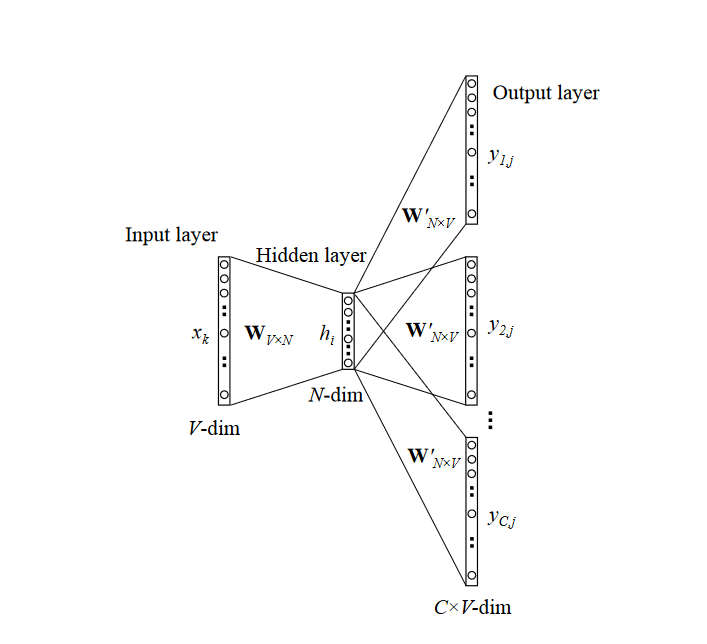
\includegraphics[scale=0.75]{modelskipgram}
\caption{Model \textit{Skip-Gram}}
\label{modelskipgram}
\end{figure}

Model ini, kebalikan dari CBOW, memiliki kata target di \textit{input layer} dan kata konteks di \textit{output layer}. \textit{Hidden layer} memiliki \textit{output} yang sama dengan CBOW, yang berarti h hanya menyalin (dan transpos) baris dari \textit{weight input}-$>$\textit{hidden matrix}, $W$, dengan \textit{input} kata $w_i$

\begin{equation}
\text{h} = \text{v}_{w_I}^T \label{eq9}
\end{equation}

untuk \textit{output layer}, karena \textit{Skip-Gram} memiliki satu \textit{input} kata dan konteks kata yang berbeda, maka hasil \textit{output layer}-nya semua sama

\begin{align}
u_{c,j} = u_j = \text{v}_{w_j}^T \cdot \text{\textbf{h}} && \text{for $c$} = 1, 2, ..., C \label{eq10}
\end{align}

dimana $u_{c,j}$ merupakan hasil keluaran perkalian antara \textbf{h}, \textit{hidden layer} dan $\text{v}_{w_j}^T$.\\
$\text{v}_{w_j}^T$ merupakan hasil perkalian \textit{input} vektor dan \textit{input weight} matriks ke-$j$ di panel \textit{output layer} ke-$c$. \\Untuk \textit{output layer} :

\begin{equation}
y_{c,j} = \frac{\text{exp}(u_{c,j})}{\sum_{j'=1}^V \text{exp}(u_j')} \label{eq11}
\end{equation}

sama seperti CBOW, \textit{Skip-Gram} menggunakan \textit{softmax} untuk \textit{output layer}. \\Dimana $y_{c,j}$ merupakan \textit{output} dari \textit{input} kata ke-$j$ dengan konteks ke-$c$.\\ $y_{c,j}$ memiliki hasil \textit{output} yang sama semua karena kata \textit{input}-nya hanya satu. Masing-masing \textit{output} akan dibandingkan dengan vektor konteks kata $C$ yang sebenarnya, yang akan menghasilkan vektor-vektor yang berbeda, yang pada akhirnya akan dijumlahkan untuk meng-\textit{update weight matrix} model ini.
\newline
\newline


\textbf{\textit{Update matrix weight hidden}-$>$\textit{output}}

\begin{align}
{V'_{w_j}}^{\text{(new)}} = {V'_{w_j}}^{\text{(old)}} - \eta \cdot \text{EI}_j \cdot \text{\textbf{h}} && \text{for $j$} = 1, 2, ..., V. \label{eq12}
\end{align}

Dimana EI merupakan $V$-dimensional vektor EI = {EI$_1$, ... , EI$_V$ }, yang merupakan total dari $e_{c,j}$. \\$e_{c,j}$ merupakan \textit{prediction error} semua kata konteks

\begin{equation}
\text{EI}_j=\sum_{c=1}^C e_{c,j} \label{eq13}
\end{equation}

\begin{equation}
e_{c,j}= y_{c,j}-t_{c,j} \label{eq14}
\end{equation}

$e_{c,j}$ merupakan selisih antara probabilitas prediksi dan \textit{true vector} (vektor yang sebenarnya).
\\ \textit{True vector} merupakan \textit{one-hot encode} kata konteks ke-$c$.
\newline
\newline


\textbf{\textit{Update matrix weight input}-$>$\textit{hidden}}

\begin{equation}
{V^{\text{(new)}}_{w_I}} = {V^{\text{(old)}}_{w_I}} - \eta \cdot \text{EH}^T \label{eq15}
\end{equation}

Dimana EH merupakan $N$-dimension vektor yang setiap isinya didefinisikan dengan

\begin{equation}
\text{EH}_i = \sum_{j=1}^V \text{EI}_j \cdot w'_{ij} \label{eq16}
\end{equation}

Persamaan EI sama dengan persamaan \eqref{eq13}.
\end{enumerate}

%\subsection{\textit{Precision}}
%Dalam IR, \textit{precision} merupakan persentase hasil dokumen yang relevan terhadap kueri. \textit{Precision} didapatkan dari jumlah hasil yang relevan dibagi dari jumlah hasil yang didapatkan. \textit{Precision at k} (P@k) merupakan \textit{precision} yang hanya menghitung relevansi terhadap k dokumen teratas.

%\begin{equation}
%\text{p} = \frac{| \text{\{dokumen relevan\}} \cap \text{\{dokumen keluaran\}}|}{|\text{\{dokumen keluaran\}}|}
%\end{equation}

\subsection{\textit{Euclidean Distance}}
Euclidean distance merupakan rumus untuk mengukur jarak antara dua vektor. Nilai yang semakin kecil berarti vektor semakin dekat. Euclidean distance akan digunakan untuk mengukur jarak antara hasil prediksi dengan vektor yang sebenarnya.

\begin{equation}
d(p,q) = \sqrt{(p_1-q_1)^2 + (p_2-q_2)^2 + ... + (p_n-q_n)^2}
\end{equation}

dimana $p$ merupakan vektor pertama dan $q$ merupakan vektor kedua

\subsection{\textit{Hit Rate}}
\textit{Hit Rate} merupakan pembagian dari \textit{user} yang dimana jawaban benarnya termasuk dalam daftar rekomendasi terhadap total \textit{user}. \textit{Hit Rate} akan digunakan untuk mengukur kesesuaian sistem pencarian terhadap \textit{user}.

\begin{equation}
HR = \frac{|U^L_{hit}|}{|U^{all}|}
\end{equation}

dimana $U^L_{hit}$ merupakan jumlah \textit{user} yang memberikan jawaban yang benar 

dalam top L rekomendasi.

$U^{all}$ merupakan total \textit{user} dalam tes.

\newpage
\section[METODOLOGI PENELITIAN]{BAB III}
\section*{METODOLOGI PENELITIAN}
\thispagestyle{plain}
\subsection{Metodologi Pengembangan Sistem}

Pada subbab ini akan dijelaskan proses yang digunakan untuk melakukan pencarian dengan menggunakan Model CBOW dan \textit{Skip-Gram}. Sistem akan dibuat dalam bentuk terminal dengan bahasa pemrograman Phyton versi 3.9.1 dan local web server Apache dengan penyimpanan data dalam bentuk database MySQL, dengan menggunakan aplikasi XAMPP.

\begin{figure}[H]
\centering
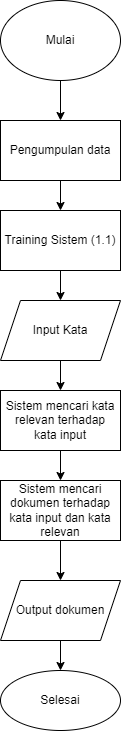
\includegraphics[scale=0.73]{prosessistemrev3}
\caption{Proses Sistem}
\label{prosessistem}
\end{figure}

Perancangan sistem akan dimulai dengan pengumpulan data. Data akan dikumpulkan dengan \textit{web crawl} lalu akan dirapihkan dengan menghapus hal-hal yang tidak berkaitan dengan artikel, contohnya teks iklan, rekomendasi judul artikel lain, dan yang lainnya. Data yang sudah dikumpulkan dan diraphikan akan disimpan ke dalam \textit{database}. Data yang dikumpulkan merupakan data yang akan dijadikan sebagai target pencarian pada sistem \textit{search engine}.

Selanjutnya \textit{Training} Sistem. Sistem akan dilatih dengan menggunakan kumpulan dokumen yang telah dikumpulkan, dengan metode CBOW dan \textit{Skip-Gram}. Masing-masing pelatihan data dilakukan untuk menemukan kata relevan terhadap kata \textit{input} berdasarkan arsitektur model, CBOW untuk menemukan kata target dari kata \textit{input} sekitar, dan \textit{Skip-Gram} untuk menemukan kata konteks sekitar dari kata \textit{input}. Setelah sistem di latih sistem dapat digunakan untuk pencarian.

Proses selanjutnya \textit{Input} Kata, \textit{user} memasukkan kata \textit{input} pada \textit{search engine} untuk mencari dokumen yang relevan. Kata \textit{input} dibatasi maksimal tiga kata untuk metode \textit{Skip-Gram} dan dua atau empat kata untuk metode CBOW dan metode gabungan \textit{Skip-Gram} dan CBOW. Setelah kata di \textit{input}, sistem akan mencari kata relevan terhadap kata \textit{input} berdasarkan metode yang digunakan. Kata relevan yang ditemukan sistem akan digunakan untuk pencarian dokumen oleh sistem. Dokumen yang memiliki kata \textit{input} dan kata relevan dengan frekuensi kemunculan tinggi akan diberikan \textit{ranking} tinggi pada \textit{output} pencarian sistem. Lima hasil dokumen dengan \textit{ranking} tertinggi yang dikeluarkan sistem akan dinilai relevansinya oleh \textit{user}.

\subsection{Analisis Data}
Tahap pertama dalam rancangan eksperimen adalah pengumpulan dataset. Dataset yang penulis pakai merupakan kumpulan artikel yang didapat dari situs : \textit{https://www.indosport.com}, yang di \textit{crawl} dengan menggunakan \textit{tools} yang dirancang oleh Muhammad Fathan Qoriiba pada skripsinya PERANCANGAN \textit{CRAWLER} SEBAGAI PENDUKUNG PADA \textit{SEARCH ENGINE}.

\subsection{Proses \textit{Training}}
\begin{figure}[H]
\centering
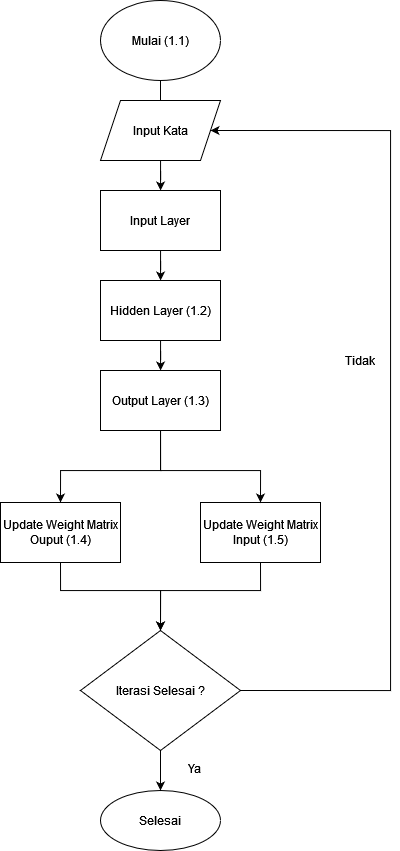
\includegraphics[scale=0.60]{prosestrainingrev4}
\caption{Proses \textit{Training}}
\label{prosestraining}
\end{figure}

	Proses \textit{Training} akan dilakukan untuk semua data yang telah dikumpulkan. Data yang telah dikumpulkan akan dibuat \textit{dictionary}, yaitu kumpulan data semua kata unik yang muncul di kumpulan dokumen/artikel tersebut. \textit{Dictionary} akan diubah ke dalam bentuk \textit{one-hot encode} sesuai indeks kata untuk digunakan dalam proses \textit{training} data ( contohnya {1 0 0 0} untuk kata di indeks pertama dengan \textit{dictionary} yang berisi empat kata). Proses \textit{training} sepenuhnya menggunakan kata yang direpresentasikan dalam bentuk \textit{one-hot encode}.



Data akan digabung menjadi satu dokumen, lalu \textit{training} akan berjalan dari awal kata hingga akhir kata pada akhir dokumen. \textit{Training} akan dijalankan sesuai model masing-masing, untuk model \textit{Skip-Gram} kata tengah sebagai kata \textit{input} dan kata sekitar sebagai kata konteks, dan untuk CBOW kata sekitar sebagai kata \textit{input} dan kata tengah sebagai kata target. Dalam \textit{input layer} kita hanya akan memasukkan \textit{one-hot encode} kata ke dalam proses \textit{training} yang selanjutnya akan digunakan ke dalam perhitungan masing-masing model, CBOW dan \textit{Skip-Gram}.

\subsubsection{\textit{Hidden Layer}}
\begin{figure}[H]
\centering
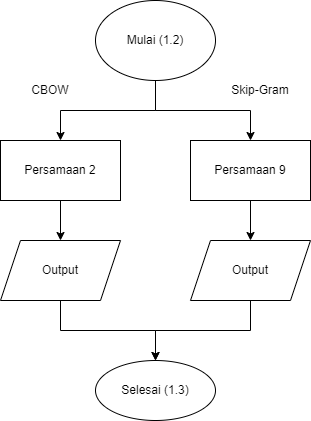
\includegraphics[scale=0.8]{hiddenlayerrev3}
\caption{\textit{Hidden Layer}}
\label{hiddenlayer}
\end{figure}
Dalam \textit{hidden layer}, masing-masing \textit{one-hot encode} kata pada masing-masing model di projeksi dengan \textit{weight matrix input} yang sebelumnya terlebih dahulu di inisiasi dengan angka acak. 

Dalam Model CBOW, kata sekitar (kata konteks) akan dimasukkan ke dalam persamaan \eqref{eq2}, yang berarti merata-ratakan vektor kata konteks berdasarkan jumlah kata konteks yang dimasukkan yang lalu akan di transpos. 

Dalam \textit{Skip-Gram}, persamaan \eqref{eq9} berarti hanya men-transpos vektor kata \textit{input} yang dimasukkan ke dalam model ini, karena model ini hanya bisa menerima satu \textit{input} kata. Kedua model masing-masing akan menghasilkan \textit{output} satu vektor kata yang akan dimasukkan ke dalam \textit{Output Layer}.

\subsubsection{\textit{Output Layer}}
\begin{figure}[H]
\centering
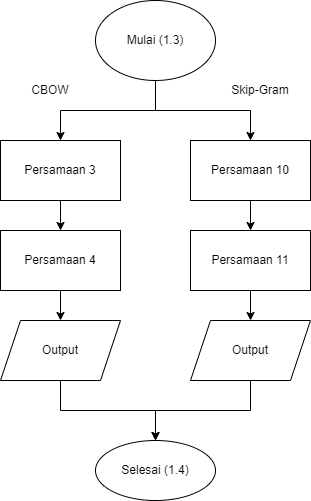
\includegraphics[scale=0.75]{outputlayerrev3}
\caption{\textit{Output Layer}}
\label{outputlayer}
\end{figure}
Hasil vektor kata dari \textit{hidden layer} pada masing-masing model akan dikalikan dengan \textit{weight matrix output} masing-masing yang sebelumnya terdahulu di inisiasi dengan angka acak.

Dalam CBOW, seperti persamaan \eqref{eq3}, vektor kata \textit{hidden layer} dikalikan dengan \textit{weight matrix output} yang akan menghasilkan $u_j$, yang akan digunakan dengan \textit{softmax function} \eqref{eq4}, yang hasilnya, $y_j$ merupakan probabilitas vektor kata. 

Sama seperti CBOW, persamaan \eqref{eq10} pada \textit{Skip-Gram} berarti perkalian hasil \textit{hidden layer} dengan \textit{weight matrix output}. Karena \textit{Skip-Gram} memiliki banyak konteks kata, $u_{c,j}$ di lakukan untuk semua $c$, yaitu untuk semua kata konteks, tapi karena \textit{input} katanya sama untuk banyak konteks kata, hasilnya semua sama, yang berarti $u_{c,j} = u_j$. $u_j$ akan dimasukkan ke dalam \textit{softmax function} yaitu persamaan \eqref{eq11} untuk mendapatkan hasil $y_{c,j}$, yaitu probabilitas vektor kata berdasarkan $c$ konteks kata.

Setelah \textit{training} kata, sistem akan melakukan \textit{backpropagation} untuk memperbaiki \textit{weight matrix} per iterasi untuk mengubah hasil \textit{output layer} agar semakin dekat dengan \textit{true vector}, yaitu \textit{one-hot encode} kata target untuk CBOW dan \textit{one-hot encode} kata konteks untuk \textit{Skip-Gram}.

\subsubsection{\textit{Update Weight Matrix Output}}
\begin{figure}[H]
\centering
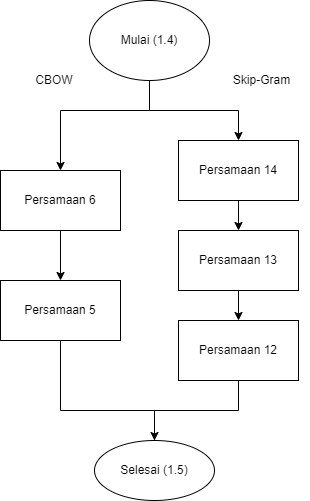
\includegraphics[scale=0.75]{updateweightoutputrev2}
\caption{\textit{Update Weight Matrix Output}}
\label{updateweightoutput}
\end{figure}
Setelah sistem di latih, hasil dari \textit{output layer} digunakan untuk meng-\textit{update weight matrix output}. Dalam model CBOW kita menggunakan persamaan \eqref{eq6} untuk mendapatkan \textit{error prediction}, dengan mengurangi hasil \textit{output layer} dengan \textit{true vector} kata target. Setelah mendapatkan $e_j$, kita dapat menggunakan persamaan \eqref{eq5} untuk mendapatkan \textit{weight matrix output} baru. 

Sedangkan untuk \textit{Skip-Gram}, karena model ini memiliki konteks kata yang banyak, \textit{error prediction} $e_{c,j}$ didapatkan per-$c$, perkonteks kata seperti persamaan \eqref{eq14}, lalu semua \textit{error prediction} dijumlahkan seperti pada persamaan \eqref{eq13}, yang hasilnya akan dimasukkan ke persamaan \eqref{eq12} untuk mendapatkan \textit{weight matrix output} baru model \textit{Skip-Gram}.

\subsubsection{\textit{Update Weight Matrix Input}}
\begin{figure}[H]
\centering
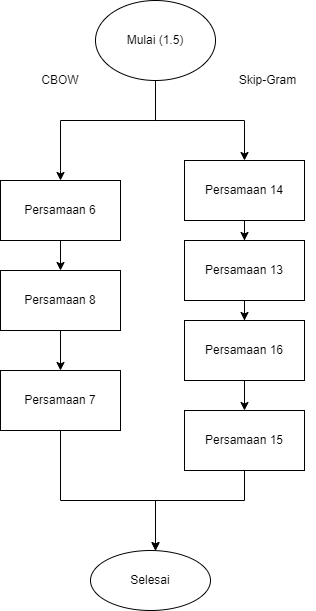
\includegraphics[scale=0.75]{updateweightinputrev2}
\caption{\textit{Update Weight Matrix Input}}
\label{updateweightinput}
\end{figure}
Di proses ini kita akan meng-\textit{update weight matrix input}. Model CBOW dimulai dengan persamaan \eqref{eq6}, sama seperti \textit{Update Weight Matrix Output}, kita mencari \textit{error prediction} yang akan kita masukkan ke persamaan \eqref{eq8}. Persamaan \eqref{eq8} berarti perkalian \textit{error prediction} dengan \textit{matrix weight output} yang hasilnya akan kita masukkan ke dalam persamaan \eqref{eq7}. Di persamaan \eqref{eq7}, $Vw_{I,c}$ berarti vektor konteks \textit{input} kata ke-$c$, yang berarti kita akan meng-\textit{update} semua vektor \textit{weight matrix input} yang merepresentasikan konteks kata yang kita masukkan ke model ini. 

Untuk model \textit{Skip-Gram}, sama seperti \textit{Update Weight Matrix Output}, kita menggunakan persamaan \eqref{eq14} yang hasilnya akan kita masukkan ke persamaan \eqref{eq13}. Hasil dari persamaan ini akan kita lakukan perkalian dengan \textit{matrix weight output} seperti persamaan \eqref{eq16} dan hasilnya akan kita masukkan ke dalam persamaan \eqref{eq15}. Mirip seperti CBOW, di model \textit{Skip-Gram} ini kita juga akan meng-\textit{update} vektor \textit{weight matrix input} yang merepresentasikan kata yang kita masukkan ke model ini. Karena dalam model \textit{Skip-Gram} kita hanya memasukkan satu kata, maka vektor yang diubah juga hanya satu vektor, hanya vektor \textit{weight matrix input} yang merepresentasikan kata tersebut. 

\textit{Weight matrix output} dan \textit{weight matrix input} yang sudah kita \textit{update} akan kita simpan ke dalam \textit{database} yang akan digunakan untuk melakukan pencarian kata relevan terhadap kata \textit{input user} pada pencarian \textit{search engine}.

\subsubsection{Penggunaan Sistem Untuk Melakukan Pencarian}
Setelah proses \textit{training} selesai sistem dapat digunakan untuk melakukan pencarian. \textit{User} akan meng-\textit{input} kata kedalam mesin pencarian dan sistem akan memproses data. Kata yang di-\textit{input user} akan diproses mirip dengan cara \textit{training} sistem tetapi dengan menggunakan \textit{weight matrix input} dan \textit{weight matrix output} yang telah disimpan di \textit{database} setelah proses \textit{training} selesai. Proses akan berjalan hingga ke \textit{output layer} yang hasil di \textit{output layer}-nya akan di cek, dimana bagian vektor yang paling mendekati satu merupakan indeks dari kata yang paling relevan terhadap kata \textit{input}. Hal ini bisa didapatkan dari proses \textit{backpropagation} yang berusaha memperbaiki hasil \textit{output layer} sesuai dengan \textit{true vektor ( one-hot encode )} kata di sekitar kata \textit{input}. Akan dicari beberapa kata relevan dari kata \textit{input user} untuk memperluas hasil pencarian dari \textit{search engine}. Di akhir, kata relevan yang ditemukan sistem tersebut akan digabungkan dengan kata \textit{input user} untuk mencari dokumen yang relevan.

\subsubsection{Pe-\textit{ranking}-an Dokumen}
Pe-\textit{ranking}-an hasil pencarian akan dilakukan dengan mencari jumlah frekuensi kemunculan kata pada dokumen dengan menggunakan kata \textit{input user} dan kata relevan yang telah ditemukan sistem. Pada pencarian dengan menggunakan CBOW, dua kata \textit{input} yang dimasukkan \textit{user} akan di cari kata tengahnya, lalu tiga kesatuan kata tersebut akan digabungkan lalu dicari di semua dokumen. Begitu juga dengan Skip-Gram, kata yang di \textit{input} \textit{user} akan digabungkan dengan dua kata keluaran sistem lalu akan digabungkan menjadi satu kesatuan lalu di cari di seluruh dokumen. Karena Skip-Gram dan CBOW hanya dapat memprediksi kemungkinan kata yang keluar berdasarkan modelnya tanpa mengetahui tetangga yang mana yang dibagian kiri atau kanan, maka pencarian dimodifikasi dengan mencoba dua kombinasi. Untuk CBOW kata satu dan dua yang di \textit{input} \textit{user} juga akan dicari dengan cara dibalik. Contohnya kata \textit{input} saya dan bermain dengan kata tengah suka akan dicari saya suka bermain dan bermain suka saya, sedangkan Skip-Gram dua kata keluarannya yang akan dibalik, contohnya kata \textit{input} suka dengan keluaran saya dan bermain akan dicari saya suka bermain dan bermain suka saya.

\subsubsection{Data Keluaran dan Evaluasi Sistem}
Data yang dihasilkan dari mesin pencarian merupakan dokumen yang diharapkan relevan dengan pencarian \textit{user}. Sistem pencarian akan mengeluarkan lima hasil dokumen. \textit{User} akan diminta untuk memberi \textit{ranking} pada lima hasil dokumen tersebut terhadap kesesuaiannya dengan kata \textit{input}. Lalu penulis di akhir akan menilai kesesuaian \textit{ranking} dokumen keluaran sistem terhadap \textit{ranking} dokumen yang diberikan \textit{user}.

%Penilaian akan dilakukan dengan menggunakan \textit{precision} pada lima dokumen teratas (P@5). Dokumen yang ditemukan relevan terhadap pencarian oleh \textit{user} akan dihitung dan dibagi dengan jumlah dokumen yang dikeluarkan sistem pada k (dibagi lima). Semakin tinggi nilai \textit{precision} berarti semakin besar kemungkinan sistem berjalan dengan baik.

\subsection{Rancangan Eksperimen}
\renewcommand{\labelitemi}{-}
\begin{enumerate}
\item Skenario pertama (Menggunakan metode \textit{Skip-Gram})
\begin{itemize}
\item \textit{Tester} memasukkan kata \textit{input} yang sama ke dalam \textit{search engine}
\item Sistem mencari kata dengan kemiripan tinggi (kata konteks) dari kata \textit{input user}
\item Sistem melakukan pencarian dokumen terhadap kata \textit{input} dan kata konteks yang terkait
\item Pe-\textit{ranking}-an dilakukan terhadap dokumen dengan menghitung frekuensi kemunculan kata \textit{input} dan kata konteks
\item Sistem mengembalikan \textit{ranking} dokumen berdasarkan hasil tersebut
\item \textit{Tester} menilai relevansi yang dihasilkan oleh sistem
\end{itemize}
\item	Skenario kedua (Menggunakan metode \textit{Continuous Bag-of-Words})
\begin{itemize}
\item \textit{Tester} memasukkan kata \textit{input} yang sama ke dalam \textit{search engine}
\item Sistem mencari kata dengan kemiripan tinggi (kata target) dari kata \textit{input user}
\item Sistem melakukan pencarian dokumen terhadap kata \textit{input} dan kata target yang terkait
\item Pe-\textit{ranking}-an dilakukan terhadap dokumen dengan menghitung frekuensi kemunculan kata \textit{input} dan kata target
\item Sistem mengembalikan \textit{ranking} dokumen berdasarkan hasil tersebut
\item \textit{Tester} menilai relevansi yang dihasilkan oleh sistem
\end{itemize}

\item Skenario ketiga (Menggunakan gabungan metode \textit{Skip-Gram} dan \textit{Continous Bag-of-Words})
\begin{itemize}
\item \textit{Tester} memasukkan kata \textit{input} yang sama ke dalam \textit{search engine}
\item Sistem mencari kata konteks dan kata target dengan kemiripan tinggi dari kata \textit{input user}
\item Sistem melakukan pencarian dokumen terhadap kata \textit{input}, kata target, dan kata konteks terkait
\item Pe-\textit{ranking}-an dilakukan terhadap dokumen dengan menghitung frekuensi kemunculan kata \textit{input} dan kata target
\item Pe-\textit{ranking}-an juga ditemukan dengan menggunakan frekuensi kata \textit{input} dan kata konteks
\item Sistem mengembalikan \textit{ranking} dokumen berdasarkan hasil tersebut
\item \textit{Tester} menilai relevansi yang dihasilkan oleh sistem
\end{itemize}
\end{enumerate}


\newpage
\section[HASIL DAN PEMBAHASAN]{BAB IV}
\section*{HASIL DAN PEMBAHASAN}
\thispagestyle{plain}
\subsection{Data dan \textit{Training Parameter}}
Data yang digunakan merupakan kumpulan artikel yang di \textit{crawl} dari situs  \textit{https://www.indosport.com}. Data yang digunakan dibatasi sejumlah 70 artikel (70 \textit{link}) yang per-artikelnya berisi teks yang berada pada \textit{link} artikel. Data lalu akan dirapihkan dengan menghapus simbol-simbol spesial, contohnya strip (-), koma (,), petik ('), dll. Data per-artikel yang sudah dirapihkan akan digabungkan menjadi satu data besar, yaitu data yang berisi semua teks pada semua artikel. Data ini akan disimpan ke dalam \textit{database} dan akan digunakan untuk \textit{training sistem}. Berikut merupakan struktur \textit{database}.

\begin{figure}[H]
\centering
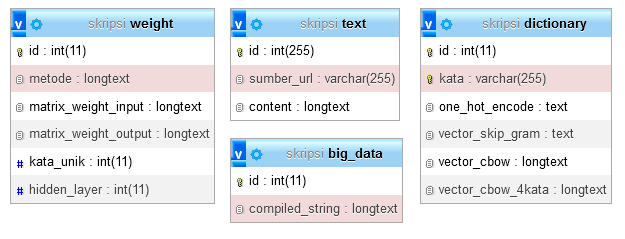
\includegraphics[scale=0.75]{struktur_database}
\caption{Struktur \textit{Database}}
\label{strukturdatabase}
\end{figure}

Tabel \textit{dictionary} merupakan tabel tempat menyimpan semua kata unik, kata unik disimpan pada kolom kata, \textit{one-hot-encode} kata disimpan pada kolom \textit{one\_hot\_encode}, dan vektor-vektor dari kata disimpan ke dalam kolom yang sesuai, vektor \textit{Skip-Gram} pada \textit{vector\_skip\_gram}, vektor CBOW dua kata pada \textit{vector\_cbow}, dan vektor CBOW empat kata pada \textit{vector\_cbow\_4kata}. Tabel \textit{big\_data} berisi kolom \textit{compiled\_string}, dimana kolom diisi oleh data gabungan yang sudah dirapihkan dari semua isi dokumen. Data ini akan digunakan untuk \textit{training sistem}. Tabel \textit{text} berisi kolom \textit{sumber\_url} dan \textit{content}, \textit{sumber\_url} berisi semua \textit{link} dari data yang di \textit{crawl} dan \textit{content} merupakan isi konten dari \textit{link} tersebut. Tabel \textit{weight} berisi nama metode, \textit{matrix\_weight\_input}, \textit{matrix\_weight\_output}, \textit{kata\_unik}, dan \textit{hidden\_layer}. Tabel ini akan digunakan untuk \textit{searching} dokumen, dimana \textit{matrix weight} yang sudah selesai di \textit{train} akan disimpan disini untuk diambil nanti pada saat pencarian teks. 

Untuk training metode \textit{Skip-Gram}, kata target \textit{training} akan dijalankan dari kata awal hingga akhir satu per satu dengan satu pasang tetangganya sebagai kata prediksi \textit{output} (satu tetangga kanan dan satu tetangga kiri). Untuk kata pada awal dan akhir data yang hanya memiliki satu tetangga (hanya sebelah kanan dan hanya sebelah kiri), kata hanya akan dilatih dengan satu tetangga tersebut.

Untuk pelatihan metode CBOW, kata yang digunakan hanya merupakan kata pertama dan ketiga dari data sebagai kata \textit{input} untuk metode CBOW dua kata, dan kata pertama, kedua, keempat, dan kelima untuk metode CBOW empat kata. Metode CBOW akan menggunakan kata tengah sebagai kata prediksi \textit{output}. \textit{Training} juga akan berjalan dari kata awal hingga akhir data, kata ketiga dihitung dari akhir data untuk metode dua kata dan kata kelima dihitung dari akhir data untuk metode empat kata.

\textit{Parameter} yang digunakan untuk \textit{training} data merupakan \textit{learning rate} sebesar 0.05 dan 400 \textit{hidden layer} (400 dimensi vektor). Dikarenakan lamanya waktu \textit{training} data, penulis memilih untuk menghapus \textit{stopwords} yang ada dalam teks. Daftar kata \textit{stopwords} yang dihapus didapat dari ``\textit{A Study of Stemming Effects on Information Retrieval in Bahasa Indonesia}'', \shortciteA{stopwords}. Kata yang hanya berisi angka juga dihapus karena dianggap tidak memiliki makna (contohnya kata ''10:43'').

Sistem terbagi menjadi tiga bagian : pembersihan data, \textit{training} data, dan program pencarian. Pembersihan data terdiri dari satu kode skrip Python : \textit{onehotencode.py}, \textit{training} data terdiri dari tiga kode skrip : \textit{training.py, trainingcbow.py, trainingcbow4kata.py} dan program pencarian terdiri dari tiga kode skrip : \textit{search.py, search2cbow.py} dan \textit{search4cbow.py}.

\subsection{Pembersihan Data}
Pada pembersihan data, \textit{onehotencode.py} berfungsi untuk memindahkan dan merapihkan data yang sudah di \textit{crawl}. Berikut akan dijelaskan fungsi \textit{onehotencode.py}. \textit{onehotencode.py} akan mengambil sampel \textit{random} data sebanyak 70 data artikel/dokumen dari data yang di \textit{crawl}. Data ini per dokumennya berisi paragraf kata. Data yang diambil akan dihapus simbol-simbol spesialnya dari kata dan akan dihapus \textit{stopwords}-nya dari paragraf. Data juga akan dirapihkan dengan menghapus \textit{whitespace} yang berlebihan (\textit{double whitespace} atau lebih) pada paragraf. Kata yang hanya terdiri dari angka juga akan dihapus. Paragraf yang sudah rapih akan digabungkan dengan paragraf-paragraf dari artikel lain lalu disimpan ke dalam tabel \textit{big\_data}. Paragraf besar ini akan digunakan untuk pelatihan sistem. Data yang sudah dirapihkan per-paragraf juga akan dimasukkan ke \textit{database} tabel \textit{text} dengan format sumber, isi. Tabel ini akan digunakan untuk pencarian dokumen dengan kata pada tahap akhir.

\begin{figure}[H]
\centering
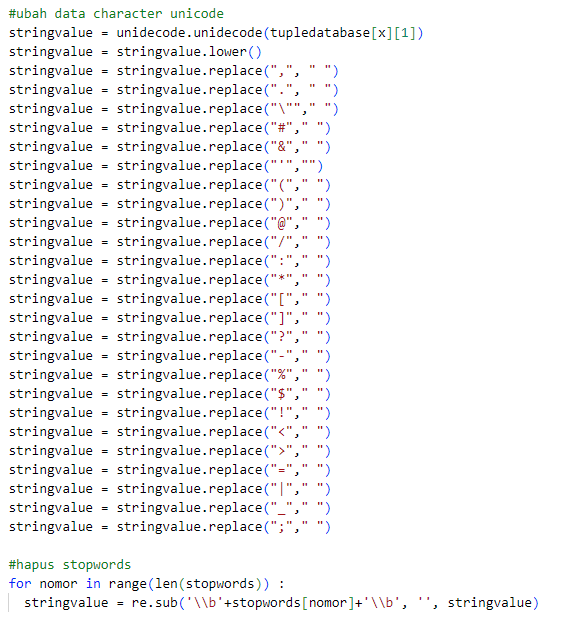
\includegraphics[scale=0.75]{pembersihan_data}
\caption{Pembersihan Data}
\label{pembersihandata}
\end{figure}

Setelah data paragraf disimpan, \textit{onehotencode.py} akan mengambil kata unik pada semua data. Semua kata unik akan dikumpulkan lalu dibuat \textit{one-hot-encode}-nya. Total kata unik yang di dapatkan setelah data di bersihkan di dapat 4199 total kata. Kata unik dan \textit{one-hot-encode} kata tersebut lalu akan disimpan di \textit{database} pada tabel \textit{dictionary}. Tabel ini akan digunakan sebagai tabel \textit{lookup one-hot-encode} dari kata pada saat proses \textit{training} dan \textit{searching}.

\begin{figure}[H]
\centering
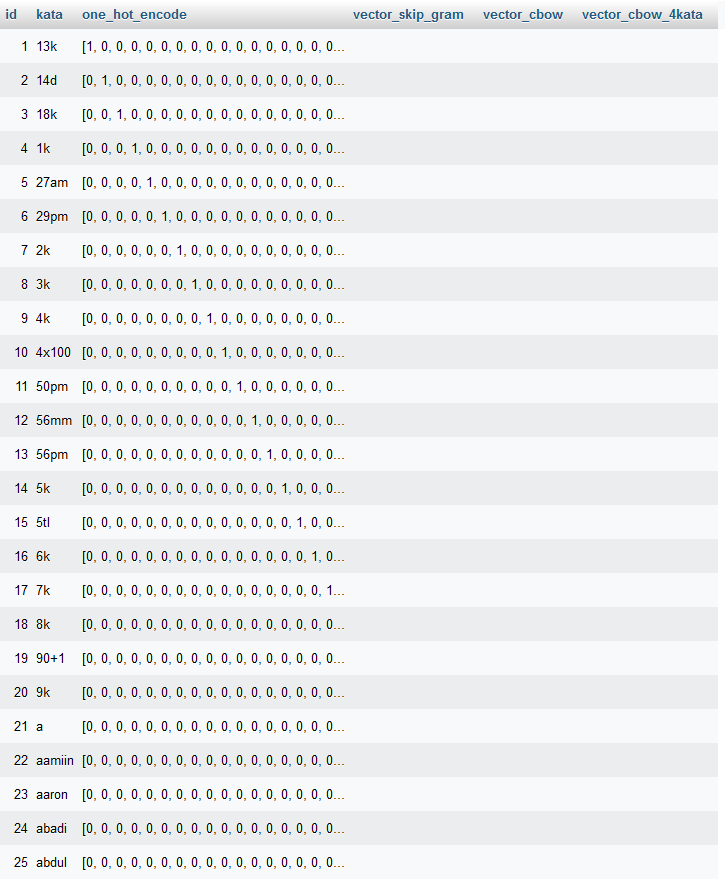
\includegraphics[scale=0.6]{listkatadanonehotencode}
\caption{Contoh \textit{List} Kata dan \textit{One-Hot-Encode}}
\label{listkatadanonehotencode}
\end{figure}

\subsection{\textit{Training Data}}
\textit{Training} data terdiri dari tiga kode skrip, yaitu \textit{training.py, trainingcbow.py}, dan \textit{trainingcbow4kata.py}. Berikut akan dijelaskan fungsi \textit{training.py}. \textit{Training.py} berfungsi untuk melatih data dengan model \textit{Continous Skip-Gram}. Pada awalnya \textit{training.py} akan menginisiasi \textit{matrix weight input} dan \textit{output} secara \textit{random}, dengan ukuran \textit{matrix weight input} 4199x400 (jumlah kata unik x \textit{hidden layer}) dan ukuran \textit{matrix weight output} 400x4199 (\textit{hidden layer} x jumlah kata unik). Skrip ini juga akan mengambil data kata unik, \textit{one-hot-encode} dan paragraf besar berisi semua kata dari tabel \textit{dictionary} dan \textit{big\_ data} pada \textit{database} secara berurutan.

\begin{figure}[H]
\centering
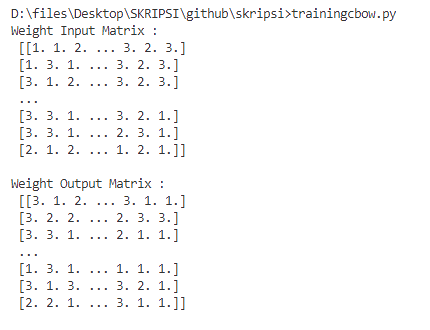
\includegraphics[scale=0.75]{inisiasi_weight}
\caption{Inisiai \textit{Weight} Secara \textit{Random}}
\label{inisiasiweight}
\end{figure}

\textit{Training} akan berjalan pada \textit{big\_data} perkata, kata pertama akan dicari \textit{one-hot-encode}-nya pada \textit{dictionary} lalu \textit{one-hot-encode} kata akan dikalikan dengan transpos \textit{weight matrix input}. Hasilnya (\textit{hidden layer}), akan dikalikan dengan transpos dari \textit{weight output matrix}. Hasil perkalian ini akan di \textit{softmax} untuk mendapatkan prediksi. Prediksi akan dikurangi dengan \textit{one-hot-encode} kata sebenarnya (kata tetangga dari kata \textit{input}). Hasil pengurangan prediksi dengan kata sebenarnya akan di total, lalu hasilnya akan digunakan untuk \textit{backpropagation}. 


\begin{figure}[H]
\centering
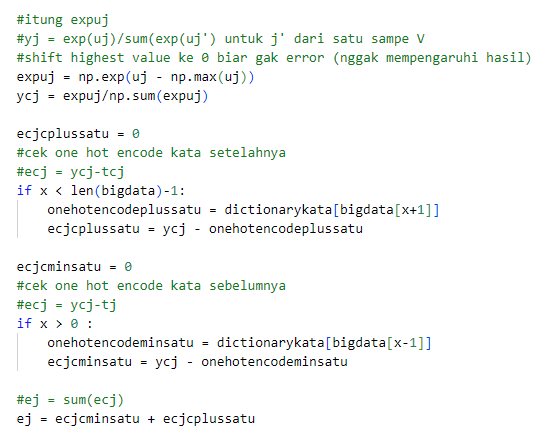
\includegraphics[scale=0.75]{softmaxlaluerror}
\caption{Mencari \textit{Softmax} Lalu Mengurangi Hasilnya dengan Angka Sebenarnya}
\label{softmaxlaluerror}
\end{figure}

Pada \textit{backpropagation, hidden layer} akan dikalikan dengan total \textit{error} dan \textit{learning rate}, lalu hasilnya akan digunakan untuk meng-\textit{update matrix weight output}. Sedangkan untuk \textit{matrix weight input}, \textit{matrix weight output} sebelum di \textit{update} akan dikalikan dengan total \textit{error}, lalu di transpos lalu dikalikan dengan \textit{learning rate}. Vektor hasil akan digunakan untuk meng-\textit{update} vektor pada \textit{matrix weight input} yang merepresentasikan kata yang di-\textit{input}. 

Setelah \textit{training} selesai \textit{matrix weight input} dan \textit{matrix weight output} yang sudah di \textit{update} akan disimpan ke dalam \textit{database}, ke dalam tabel \textit{weight}. Tabel ini akan digunakan untuk \textit{searching} pada tahap akhir. Sebelum dimasukkan ke dalam \textit{database, weight matrix input} dan \textit{matrix weight output} akan di \textit{flatten} agar \textit{formatting} lebih gampang pada saat \textit{search} nanti. Tabel \textit{dictionary} juga akan di \textit{update} pada bagian \textit{vector\_skip\_gram} dengan isi vektor pada \textit{matrix weight input} yang merepresentasikan kata.

\begin{figure}[H]
\centering
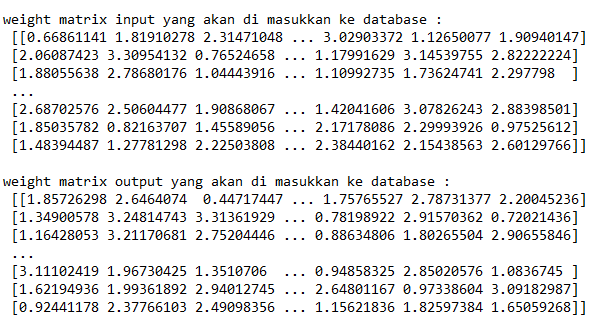
\includegraphics[scale=0.75]{weight_matrix yang_sudah_di_update}
\caption{\textit{Weight Matrix} Setelah \textit{Training}}
\label{weightmatrixyangsudahdiupdate}
\end{figure}


Untuk \textit{trainingcbow.py} fungsinya juga sama, yaitu \textit{training} kata. Bedanya ia dengan menggunakan model CBOW. Dua kata dicari \textit{one-hot-encode}-nya lalu dirata-ratakan, lalu dikalikan dengan \textit{matrix weight input}. Hasil \textit{hidden layer} dikalikan dengan \textit{matrix weight output} lalu hasilnya di \textit{softmax} untuk mendapatkan prediksi. Prediksi akan dibandingkan dengan kata sebenarnya, yaitu kata tengah dari dua kata yang di-\textit{input}. Hasil \textit{error}-nya akan digunakan untuk \textit{backpropagation}. Fungsi ini juga memiliki \textit{backpropagation} yang mirip, kecuali pada bagian \textit{update weight matrix input} dimana dia meng-\textit{update} dua vektor, yaitu vektor pada \textit{matrix weight input} yang merepresentasikan dua kata \textit{input} yang kita masukkan. Untuk \textit{trainingcbow4kata.py}, fungsi hampir semua sama dengan \textit{trainingcbow.py}, bedanya hanya kata \textit{input}-nya yang empat kata dan \textit{update} pada empat vektor yang merepresentasikan empat kata yang dimasukkan. Setelah selesai \textit{training}, \textit{matrix} akan di \textit{flatten} lalu dimasukkan ke dalam \textit{database}.

Dipilih waktu tiga jam untuk melakukan \textit{training} kedua sistem. Digunakan \textit{Euclidean Distance} untuk menghitung jarak dari hasil akhir (hasil prediksi \textit{softmax}) dan hasil sebenarnya (\textit{one-hot-encode} kata output). Pada \textit{training} sistem \textit{Skip-Gram}, hasil berhenti pada jarak tetangga kiri 0.87 dan tetangga kanan 0.9 setelah tiga jam dengan 43 iterasi. Sedangkan CBOW menghasilkan 0.1 untuk metode dua kata setelah tiga jam dilatih dengan 50 iterasi dan 0.067 untuk metode empat kata setelah tiga jam dan 29 iterasi. Hasil jarak pada \textit{Skip-Gram} dianggap terlalu jauh dan tidak layak digunakan untuk sistem pencarian.

\subsection{Pencarian Kata Pada Dokumen}
Program pencarian terdiri dari tiga kode skrip : \textit{search.py, search2cbow.py} dan \textit{search4cbow.py}. \textit{search.py} melakukan pencarian dengan metode \textit{Skip-Gram}, \textit{searchcbow.py} melakukan pencarian dengan metode CBOW dua kata, dan \textit{search4cbow.py} melakukan pencarian dengan CBOW metode empat kata. Ketiga program ini berbentuk terminal.

\begin{figure}[H]
\centering
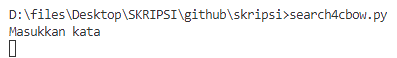
\includegraphics[scale=0.75]{prompt_user}
\caption{Program Pencarian Berbasis Terminal}
\label{promptuser}
\end{figure}

Pada \textit{search.py}, pertama program akan mengambil \textit{matrix weight input} dan \textit{matrix weight output} yang sudah di \textit{update} dari \textit{database}. \textit{Weight} yang sudah di \textit{flatten} dari \textit{database} di \textit{format} kembali menjadi \textit{matrix} dengan parameter \textit{kata\_unik} dan \textit{hidden\_layer} dari tabel \textit{weight} itu juga. Skrip ini juga akan mengambil \textit{one-hot-encode} dan semua jenis kata unik dari tabel \textit{dictionary} pada \textit{database}. 

Program akan menampilkan \textit{prompt user} untuk meng-\textit{input} satu kata. Setelah kata di-\textit{input} skrip akan mencari \textit{one-hot-encode} dari kata \textit{input user}. Program akan dijalankan seperti pada saat \textit{training Skip-Gram}. \textit{One-hot-encode} akan dikalikan dengan \textit{matrix weight input}, lalu hasilnya, \textit{hidden layer} akan dikalikan dengan \textit{matrix weight output}. Lalu hasil dari perkalian ini akan di \textit{softmax}.

Di \textit{softmax} kita akan mencari dua nilai yang paling mendekati satu, dimana indeks dari dua nilai tersebut merupakan kata yang seharusnya kata tetangga dari kata \textit{input}. Kata ini akan digabungkan dengan kata \textit{input} (kata \textit{input} di tengah dengan dua kata temu di sekitar) lalu skrip akan mengambil data dari tabel \textit{text} pada \textit{database}, dimana tabel berisi semua sumber dan isi artikel. Di akhir, skrip akan melakukan pencarian tiga kata pada isi artikel dimana artikel dengan kemunculan kata paling tinggi akan menjadi dokumen dengan urutan paling tinggi.

\begin{figure}[H]
\centering
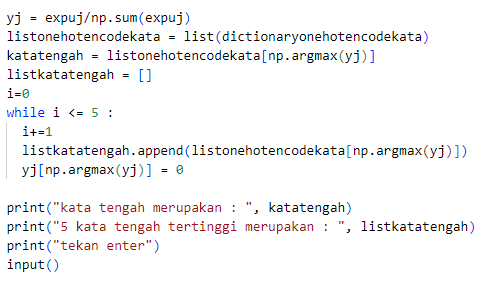
\includegraphics[scale=0.75]{pencarian_kata_tengah}
\caption{Pencarian Kata Tengah pada CBOW dengan Mencari Indeks Angka Paling Besar pada Hasil \textit{Softmax}}
\label{pencarian_kata_tengah}
\end{figure}

\begin{figure}[H]
\centering
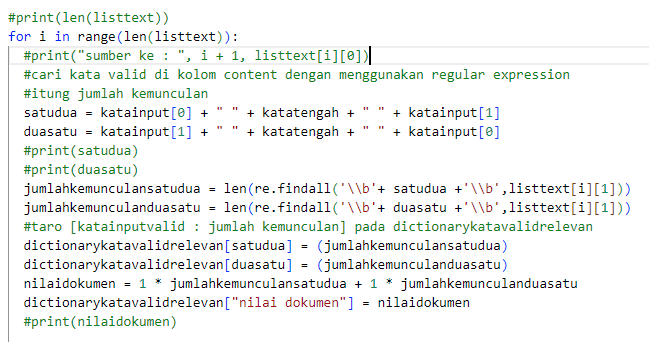
\includegraphics[scale=0.75]{pencarian_dengan_regex}
\caption{Pencarian Kata pada Semua Dokumen Menggunakan \textit{Regular Ekspression}}
\label{pencarian_dengan_regex}
\end{figure}

\begin{figure}[H]
\centering
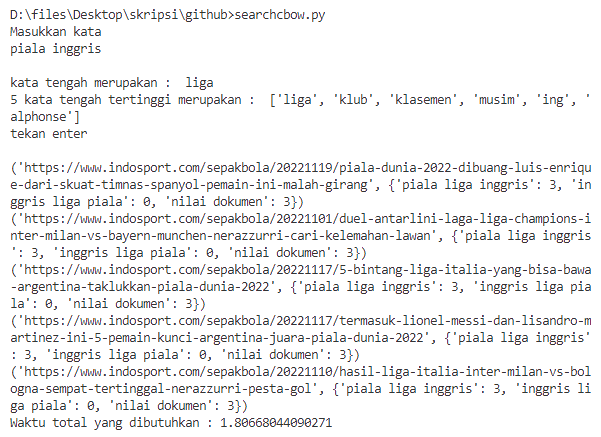
\includegraphics[scale=0.75]{contoh_hasil_pencarian}
\caption{Contoh Hasil Pencarian Dokumen}
\label{contohhasilpencarian}
\end{figure}

\textit{searchcbow.py} mirip dengan \textit{search.py} dimana bedanya ia perlu meng-\textit{input} dua kata dengan \textit{output} satu kata. Ketiga kata keluaran akan digabung (kata keluaran di tengah-tengah kata \textit{input}) lalu akan dicari dokumen mana yang memiliki kemunculan paling tinggi. \textit{search4cbow.py} hampir sama dengan beda kata \textit{input} yang dibutuhkan merupakan empat.


\subsection{Pengetesan \textit{User}}
Pengetesan akan dilakukan terhadap tiga \textit{user} terhadap tiga eksperimen, metode \textit{Skip-Gram}, metode CBOW, dan metode gabungan. \textit{User} akan diminta meng-\textit{input} kata yang sama ke dalam program lalu \textit{user} akan diminta untuk memberikan \textit{ranking} pada lima hasil dokumen yang keluar. Selanjutnya penulis akan menilai \textit{ranking} pencarian dokumen yang dikeluarkan sistem terhadap \textit{ranking user}. \textit{User} akan diminta mengisi kuisioner tentang relevansi hasil dokumen pada sistem.

\begin{figure}[H]
\centering
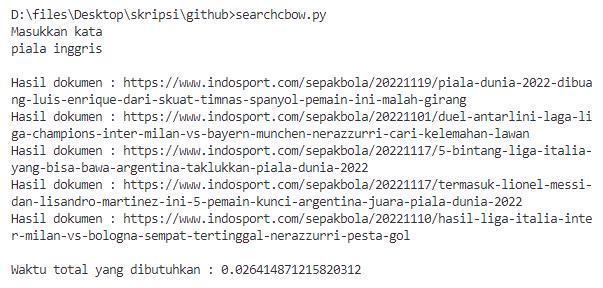
\includegraphics[scale=0.75]{contoh_hasil_pencarian_pada_user}
\caption{Contoh Hasil Pencarian Dokumen oleh \textit{User}}
\label{contohhasilpencarianolehuser}
\end{figure}

\subsection{Analisis Hasil}
Bagian ini akan membahas hasil dari tiga eksperimen yang telah dilakukan. Hasil skenario percobaan yang pertama, pada saat pelatihan proses \textit{training Skip-Gram}, setelah tiga jam \textit{training}, hasil yang di dapat terlalu jauh dengan hasil yang seharusnya. Hasil yang di dapat merupakan jarak antara hasil prediksi dan hasil yang sebenarnya yang di hitung dengan menggunakan \textit{Euclidean Distance}. Jarak akhir yang di dapat merupakan 0.87 untuk tetangga kiri dan 0.9 untuk tetangga kanan setelah 43 iterasi selama tiga jam.  Berdasarkan landainya grafik dan hasil jarak pada \textit{Skip-Gram} yang dianggap terlalu jauh, maka sistem dianggap tidak cocok untuk skenario pengetesan. 


Untuk skenario CBOW, \textit{training} sistem \textit{input} dua kata dengan waktu tiga jam menghasilkan hasil jarak 0.1 pada iterasi 50, sedangkan \textit{training} sistem \textit{input} empat kata menghasilkan jarak akhir 0.067 dengan total 29 iterasi. Dengan hasil tersebut sistem dianggap layak untuk di tes ke \textit{user}.

\begin{figure}[H]
\centering
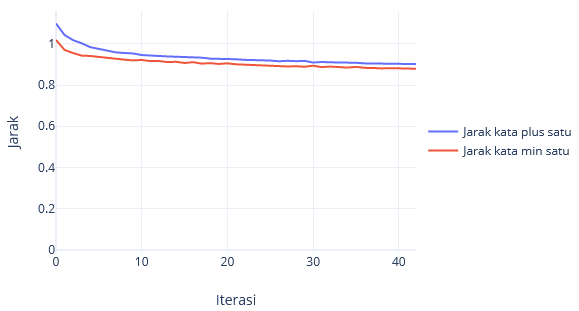
\includegraphics[scale=0.75]{jarakskipgram}
\caption{Jarak Antara Prediksi dengan Hasil Sebenarnya \textit{Skip-Gram}}
\label{jarakskipgram}
\end{figure}

\begin{figure}[H]
\centering
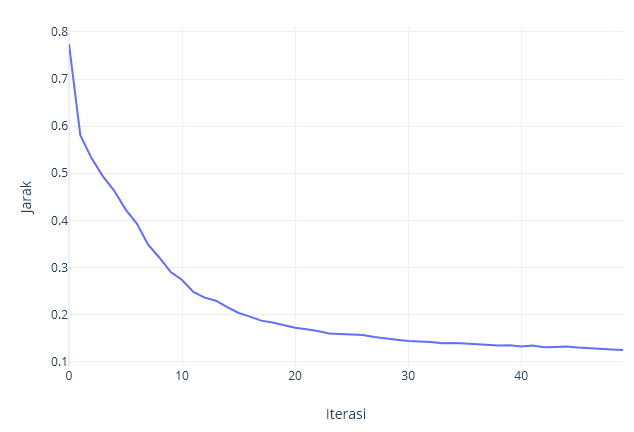
\includegraphics[scale=0.75]{jarakcbow}
\caption{Jarak Antara Prediksi dengan Hasil Sebenarnya CBOW Dua Kata}
\label{jarakcbow}
\end{figure}

\begin{figure}[H]
\centering
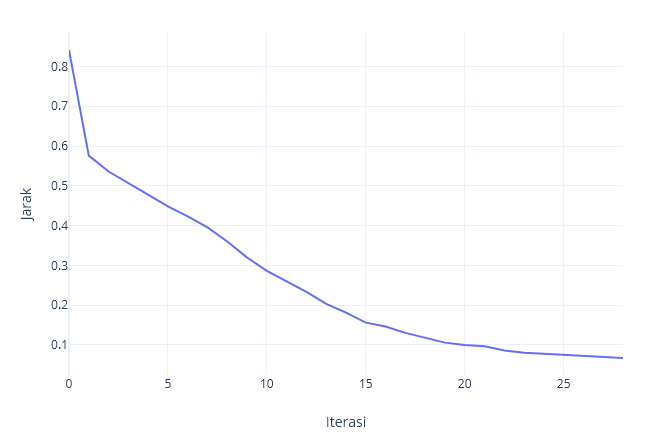
\includegraphics[scale=0.75]{jarakcbow4kata}
\caption{Jarak Antara Prediksi dengan Hasil Sebenarnya CBOW Empat Kata}
\label{jarakcbow4kata}
\end{figure}

Untuk pengetesan relevansi pencarian terhadap \textit{user} dengan menggunakan metode CBOW, \textit{user} akan diberikan lima pasang kata untuk metode CBOW dua kata, dan lima dua pasang kata untuk metode CBOW empat kata. \textit{User} akan diminta untuk memasukkan kata tersebut ke dalam mesin pencarian. Mesin pencarian akan mengeluarkan lima hasil dokumen lalu \textit{user} diminta untuk menilai \textit{ranking} dari dokumen keluaran sistem tersebut. Untuk hasil pencarian teks yang hanya menghasilkan jumlah dokumen yang kurang dari lima, sisa data akan diisi dengan dokumen random untuk dinilai oleh \textit{user}, dan untuk dokumen yang memiliki jumlah hasil kemunculan kata yang sama, dokumen akan diberikan \textit{ranking} yang sama.

Berikut akan dipaparkan hasil pencarian dengan menggunakan metode CBOW dua kata.


\begin{center}
\begin{longtable}[c]{  |  >{\raggedright\arraybackslash}m{4cm} | >{\centering\arraybackslash}m{1.3cm} | >{\centering\arraybackslash}m{1.3cm} | >{\centering\arraybackslash}m{1.3cm} | >{\centering\arraybackslash}m{1.3cm} | >{\centering\arraybackslash}m{2cm} | }
\caption{Pencarian Pertama CBOW dengan Menggunakan Kata ``hasil'' dan ``italia''}\\
\hline
\multirow{2}{4cm}{\centering{Dokumen}}								&   \multicolumn{4}{c|}{\textit{Ranking}} &\multirow{2}{2cm}{Kesesuaian} \\\cline{2-5}
																				& Sistem & \textit{User} 1 & \textit{User} 2 & \textit{User} 3& \endfirsthead
\hline
\multirow{2}{4cm}{\centering{Dokumen}}								&   \multicolumn{4}{c|}{\textit{Ranking}} &\multirow{2}{2cm}{Kesesuaian} \\\cline{2-5}
																				& Sistem & \textit{User} 1 & \textit{User} 2 & \textit{User} 3& \endhead																				
\hline
\textit{https://www.indosport. com/tag/13322/lautaro-martinez} 												&1 / 2		&1	&4 &2 &66.67\% \\
\hline
\textit{https://www.indosport. com/sepakbola/ 20221110/hasil-liga-italia-inter-milan-vs-bologna-sempat-tertinggal-nerazzurri-pesta-gol}	&1 / 2		&2	&1 &1 &100\%\\
\hline
\textit{https://www.indosport. com/sportainment/ 20200324/persija-libur-ini-yang-dilakukan-marko-simic-dan-manohara}				&x 		&3	&2 &5&x \\
\hline
\textit{https://www.indosport. com/tag/5059/kenny-sansom}												&x 		&4	&3 &4 &x \\
\hline
\textit{https://www.indosport. com/multisport/ 20190930/naik-ring-november-2019-daud-yordan-jalani-latihan-khusus-di-bali} 			&x  		&5	&5 &3 &x \\
\hline
\end{longtable}
\end{center}

Pencarian pertama dengan kata hasil dan italia menghasilkan kata tengah liga, dan kata ``hasil liga italia'' ditemukan sekali pada dua \textit{ranking} teratas dengan nilai yang sama, yaitu masing-masing dokumen ditemukan kata tersebut hanya sekali. Sedangkan tiga \textit{ranking} dibawahnya merupakan data random karena tidak ditemukan kata tersebut pada dokumen lain. Karena hasil pertama dan hasil kedua ditemukan dengan nilai yang sama, maka hasil pertama atau kedua diberikan \textit{ranking} 1 atau 2. Jika \textit{user} menilai \textit{ranking} satu atau dua pada dokumen tersebut maka hasil akan dianggap sesuai. Pada hasil kueri pertama, didapatkan dua \textit{hit} dari total tiga user, maka didapatkan \textit{hit rate} sebesar $\frac{2}3$, yang menghasilkan kesesuaian 66.67\%. Hasil kesesuaian rata-rata yang di dapat dari semua kueri merupakan 83.34\%

\newpage
\begin{center}
\begin{longtable}[c]{  |  >{\raggedright\arraybackslash}m{4cm} | >{\centering\arraybackslash}m{1.3cm} | >{\centering\arraybackslash}m{1.3cm} | >{\centering\arraybackslash}m{1.3cm} | >{\centering\arraybackslash}m{1.3cm} | >{\centering\arraybackslash}m{2cm} | }
\caption{Pencarian Kedua CBOW dengan Menggunakan Kata ``pemain'' dan ``milan''}\\
\hline
\multirow{2}{4cm}{\centering{Dokumen}}								&   \multicolumn{4}{c|}{\textit{Ranking}} &\multirow{2}{2cm}{Kesesuaian} \\\cline{2-5}
																				& Sistem & \textit{User} 1 & \textit{User} 2 & \textit{User} 3& \endfirsthead
\hline
\multirow{2}{4cm}{\centering{Dokumen}}								&   \multicolumn{4}{c|}{\textit{Ranking}} &\multirow{2}{2cm}{Kesesuaian} \\\cline{2-5}
																				& Sistem & \textit{User} 1 & \textit{User} 2 & \textit{User} 3& \endhead																				
\hline
\textit{https://www.indosport. com/sepakbola/ 20221010/prediksi-liga-champions-ac-milan-vs-chelsea-menang-atau-digilas-sejarah}				&1 / 2 / 3 &1	&1 &1 & 100\%\\	
\hline
\textit{https://www.indosport. com/sepakbola/ 20221012/tengah-main-bersama-chelsea-pierre-emerick-aubameyang-punya-karier-aneh-di-ac-milan}	&1 / 2 / 3 &2     &2 &2 & 100\%\\
\hline
\textit{https://www.indosport. com/liga-italia}																	&1 / 2 / 3 &3	&3 &3 & 100\%\\
\hline
\textit{https://www.indosport. com/sportainment/ 20221110/bertabur-bintang-indonesian-esports-awards-2022-bakal-lebih-semarak-dan-meriah}		&4 / 5    &4	&4 &4 & 100\%\\
\hline
\textit{https://www.indosport. com/multi-event/ 20191004/mencontek-gaya-hidup-sehat-ala-polisi}									&4 / 5 	 &5	&5 &5 & 100\%\\
\hline
\end{longtable}
\end{center}

Pencarian kedua dengan kata pemain dan milan menghasilkan kata tengah ac. Pencarian dengan kata ``pemain ac milan'' ditemukan dua kali pada tiga dokumen teratas, dan sekali pada dua dokumen terakhir. Dokumen hasil ke empat dan ke lima menghasilkan topik yang tidak sesuai dengan kata \textit{input} tetapi memilki hasil kemunculan satu pada tiap dokumen, hal ini disebabkan oleh sumber data yang kurang sempurna pembersihannya, dimana judul berita rekomendasi artikel lain masih berada pada isi dokumen pada saat pencarian di lakukan di sistem. Rata-rata hasil kesesuaian terakhir yang di dapat merupakan 100\%


\begin{center}
\begin{longtable}[c]{  |  >{\raggedright\arraybackslash}m{4cm} | >{\centering\arraybackslash}m{1.3cm} | >{\centering\arraybackslash}m{1.3cm} | >{\centering\arraybackslash}m{1.3cm} | >{\centering\arraybackslash}m{1.3cm} | >{\centering\arraybackslash}m{2cm} | }
\caption{Pencarian Ketiga CBOW dengan Menggunakan Kata ``juara'' dan ``dunia''}\\
\hline
\multirow{2}{4cm}{\centering{Dokumen}}								&   \multicolumn{4}{c|}{\textit{Ranking}} &\multirow{2}{2cm}{Kesesuaian} \\\cline{2-5}
																				& Sistem & \textit{User} 1 & \textit{User} 2 & \textit{User} 3& \endfirsthead
\hline
\multirow{2}{4cm}{\centering{Dokumen}}								&   \multicolumn{4}{c|}{\textit{Ranking}} &\multirow{2}{2cm}{Kesesuaian} \\\cline{2-5}
																				& Sistem & \textit{User} 1 & \textit{User} 2 & \textit{User} 3& \endhead																				
\hline
\textit{https://www.indosport. com/tag/13322/lautaro-martinez} 																&1 / 2&1&3&5&33.33\%\\
\hline
\textit{https://www.indosport. com/sepakbola/ 20221116/5-pemain-yang-bisa-bantu-lionel-messi-dan-argentina-juara-piala-dunia-2022}					&1 / 2&2&1&1&100\%\\
\hline
\textit{https://www.indosport. com/sepakbola/ 20221117/termasuk-lionel-messi-dan-lisandro-martinez-ini-5-pemain-kunci-argentina-juara-piala-dunia-2022}		&3 / 4&3&2&2&33.33\%\\
\hline
\textit{https://www.indosport. com/liga-italia}																			&3 / 4&4&4&4&100\%\\
\hline
\textit{https://www.indosport. com/multi-event/20221201/kilas-balik-setahun-sanksi-wada-gara-gara-2-atlet-pakai-doping-indonesia-kelimpungan} 			&x&5&5&3&x\\
\hline
\end{longtable}
\end{center}


Pencarian ketiga dengan kata juara dan dunia menghasilkan kata piala. Pencarian dengan kata ``juara piala dunia'' menghasilkan dua dokumen teratas dengan jumlah temu dua kali, jumlah temu sekali pada dokumen nomor tiga dan empat, dan tidak ditemukan pada dokumen lima, sehingga data diisi \textit{random}. Hasil kesesuaian rata-rata yang didapat merupakan 66.67\%. Hasil pencarian pertama merupakan \textit{landing page} untuk \textit{tag} pemain lautaro martinez, dimana \textit{webpage} berisi banyak teks ``juara'' dan ``piala dunia''. \textit{User} menganggap hasil dokumen pertama tidak mencerminkan kata ``juara'' dan ``dunia'' dibanding dokumen lain.

\newpage
\begin{center}
\begin{longtable}[c]{  |  >{\raggedright\arraybackslash}m{4cm} | >{\centering\arraybackslash}m{1.3cm} | >{\centering\arraybackslash}m{1.3cm} | >{\centering\arraybackslash}m{1.3cm} | >{\centering\arraybackslash}m{1.3cm} | >{\centering\arraybackslash}m{2cm} | }
\caption{Pencarian Keempat CBOW dengan Menggunakan Kata ``olahraga'' dan ``tinju''}\\
\hline
\multirow{2}{4cm}{\centering{Dokumen}}								&   \multicolumn{4}{c|}{\textit{Ranking}} &\multirow{2}{2cm}{Kesesuaian} \\\cline{2-5}
																				& Sistem & \textit{User} 1 & \textit{User} 2 & \textit{User} 3& \endfirsthead
\hline
\multirow{2}{4cm}{\centering{Dokumen}}								&   \multicolumn{4}{c|}{\textit{Ranking}} &\multirow{2}{2cm}{Kesesuaian} \\\cline{2-5}
																				& Sistem & \textit{User} 1 & \textit{User} 2 & \textit{User} 3& \endhead																				
\hline
\textit{https://www.indosport. com/tinju/ 20221202/jadwal-tinju-dunia-2022-duel-tak-berimbang-tyson-fury-vs-derek-chisora}						&1&1	&1&1&100\%\\
\hline
\textit{https://www.indosport. com/sepakbola/ 20220728/prediksi-liga-1-rans-nusantara-fc-vs-pss-sleman-berburu-3-poin-perdana}					&x&2	&3&5&x\\
\hline
\textit{https://www.indosport. com/sportainment/ 20220314/pakai-sport-bra-minimalis-saat-siram-tanaman-body-yeyen-lidya-makin-aduhai}				&x&3	&2&4&x\\
\hline
\textit{https://www.indosport. com/ragam/ 20221029/top-5-news-aaron-chia-sooh-woi-yik-kandas-ada-kejutan-dari-pemain-indonesia-di-luar-negeri}		&x&4	&4&2&x\\
\hline
\textit{https://www.indosport. com/sepakbola/ 20221123/sengaja-buang-cristiano-ronaldo-3-pemain-ini-diam-diam-sudah-dilirik-manchester-united}			&x&5	&5&3&x\\
\hline
\end{longtable}
\end{center}


Pencarian kata keempat, yaitu olahraga dan tinju, menghasilkan kata tengah berita. Pencarian dengan menggunakan kata ``olahraga berita tinju'' hanya menghasilkan satu dokumen, yaitu dokumen teratas dengan jumlah temu dua kali, sisa empat dokumen diisi dengan empat dokumen \textit{random}. Empat berita \textit{random} yang diisi tidak berhubungan dengan kata tinju yang menghasilkan rata-rata kesesuaian 100\%, 


\begin{center}
\begin{longtable}[c]{  |  >{\raggedright\arraybackslash}m{4cm} | >{\centering\arraybackslash}m{1.3cm} | >{\centering\arraybackslash}m{1.3cm} | >{\centering\arraybackslash}m{1.3cm} | >{\centering\arraybackslash}m{1.3cm} | >{\centering\arraybackslash}m{2cm} | }
\caption{Pencarian Kelima CBOW dengan Menggunakan Kata ``striker'' dan ``italia''}\\
\hline
\multirow{2}{4cm}{\centering{Dokumen}}								&   \multicolumn{4}{c|}{\textit{Ranking}} &\multirow{2}{2cm}{Kesesuaian} \\\cline{2-5}
																				& Sistem & \textit{User} 1 & \textit{User} 2 & \textit{User} 3& \endfirsthead
\hline
\multirow{2}{4cm}{\centering{Dokumen}}								&   \multicolumn{4}{c|}{\textit{Ranking}} &\multirow{2}{2cm}{Kesesuaian} \\\cline{2-5}
																				& Sistem & \textit{User} 1 & \textit{User} 2 & \textit{User} 3& \endhead																				
\hline
\textit{https://www.indosport. com/tag/13322/lautaro-martinez}															&1 / 2&4	&2&2&66.67\%\\
\hline
\textit{https://www.indosport. com/sepakbola/ 20221124/4-striker-liga-italia-yang-cocok-gantikan-cristiano-ronaldo-di-manchester-united}					&1 / 2&1	&1&1&100\%\\
\hline
\textit{https://www.indosport. com/sepakbola/ 20221106/harap-harap-cemas-reuni-dengan-arsenal-aubameyang-optimistis-bawa-chelsea-menang-di-kandang	}		&x&2	&3&5&x\\
\hline
\textit{https://www.indosport. com/multi-event/20221103/pelatih-timnas-indonesia-u-17-bima-sakti-ajak-anak-indonesia-rutin-cuci-tangan-pakai-sabun}				&x&3	&5&4&x\\
\hline
\textit{https://www.indosport. com/ragam/ 20221029/top-5-news-aaron-chia-sooh-woi-yik-kandas-ada-kejutan-dari-pemain-indonesia-di-luar-negeri} 				&x&5	&4&3&x\\
\hline
\end{longtable}
\end{center}

Pencarian kata kelima, dengan menggunakan kata striker dan italia, menghasilkan kata tengah liga. Pencarian dengan menggunakan kata ``striker liga italia'' menghasilkan dua dokumen teratas dengan jumlah kata temu masing-masing satu. Sisa tiga dokumen diisi dengan dokumen random. Walau nilai kemunculan sama, rata-rata \textit{user} menilai hasil dokumen dua lebih tinggi dibanding hasil dokumen pertama. Hasil rata-rata kesesuaian merupakan 83.34\%. 

Dengan itu dari lima pertanyaan total yang diberikan, hasil kesesuaian pe-\textit{ranking}-an sistem pencarian dengan menggunakan metode CBOW dua kata terhadap pe-\textit{ranking}-an \textit{user} merupakan 86.67\%.


Berikut merupakan hasil pencarian dengan menggunakan metode CBOW empat kata.


\begin{center}
\begin{longtable}[c]{  |  >{\raggedright\arraybackslash}m{4cm} | >{\centering\arraybackslash}m{1.3cm} | >{\centering\arraybackslash}m{1.3cm} | >{\centering\arraybackslash}m{1.3cm} | >{\centering\arraybackslash}m{1.3cm} | >{\centering\arraybackslash}m{2cm} | }
\caption{Pencarian Pertama CBOW dengan Menggunakan Kata ``pemain'', ``kunci'', ``juara'', dan ``piala''}\\ 
\hline
\multirow{2}{4cm}{\centering{Dokumen}}								&   \multicolumn{4}{c|}{\textit{Ranking}} &\multirow{2}{2cm}{Kesesuaian} \\\cline{2-5}
																				& Sistem & \textit{User} 1 & \textit{User} 2 & \textit{User} 3& \endfirsthead
\hline
\multirow{2}{4cm}{\centering{Dokumen}}								&   \multicolumn{4}{c|}{\textit{Ranking}} &\multirow{2}{2cm}{Kesesuaian} \\\cline{2-5}
																				& Sistem & \textit{User} 1 & \textit{User} 2 & \textit{User} 3& \endhead																				
\hline
\textit{https://www.indosport. com/tag/13322/lautaro-martinez}														&1 / 2		&3	&3 &2 &33.33\% \\
\hline
\textit{https://www.indosport. com/sepakbola/ 20221117/termasuk-lionel-messi-dan-lisandro-martinez-ini-5-pemain-kunci-argentina-juara-piala-dunia-2022}	&1 / 2		&1	&1 &1 &100\% \\
\hline
\textit{https://www.indosport. com/raket/ 20220502/sederhana-namun-tetap-khidmat-begini-suasana-perayaan-idulfitri-tim-bulutangkis-indonesia-di-manila}	&x		&2	&2 &3 &x \\
\hline
\textit{https://www.indosport. com/otomotif/ 20181031/muncul-bunyi-berisik-ini-solusi-sempurna-untuk-cvt-motor-matik}						&x 		&5	&5 &4 &x \\
\hline
\textit{https://www.indosport. com/multi-event/ 20220506/breaking-news-asian-games-hangzhou-2022-resmi-ditunda-gara-gara-covid-19}	 			&x		&4	&4 &5 &x \\
\hline
\end{longtable}
\end{center}

Pencarian kata pertama menggunakan kata pemain, kunci, juara dan piala, menghasilkan kata tengah argentina. Pencarian dengan kata ``pemain kunci argentina juara piala'' menghasilkan jumlah temu satu kali pada dokumen pertama dan kedua, dan tidak ditemukan pada dokumen lainnya. Hasil rata-rata kesesuaian merupakan 66.67\%


\newpage
\begin{center}
\begin{longtable}[c]{  |  >{\raggedright\arraybackslash}m{4cm} | >{\centering\arraybackslash}m{1.3cm} | >{\centering\arraybackslash}m{1.3cm} | >{\centering\arraybackslash}m{1.3cm} | >{\centering\arraybackslash}m{1.3cm} | >{\centering\arraybackslash}m{2cm} | }
\caption{Pencarian Kedua CBOW dengan Menggunakan Kata ``chelsea'', ``lepas'', ``abraham'', dan ``arsenal''}\\
\hline
\multirow{2}{4cm}{\centering{Dokumen}}								&   \multicolumn{4}{c|}{\textit{Ranking}} &\multirow{2}{2cm}{Kesesuaian} \\\cline{2-5}
																				& Sistem & \textit{User} 1 & \textit{User} 2 & \textit{User} 3& \endfirsthead
\hline
\multirow{2}{4cm}{\centering{Dokumen}}								&   \multicolumn{4}{c|}{\textit{Ranking}} &\multirow{2}{2cm}{Kesesuaian} \\\cline{2-5}
																				& Sistem & \textit{User} 1 & \textit{User} 2 & \textit{User} 3& \endhead																				
\hline
\textit{https://www.indosport. com/sepakbola/ 20210726/chelsea-bakal-lepas-tammy-abraham-ke-arsenal-bila-hal-ini-terwujud}				&1		&1	&1 &1 &100\% \\
\hline
\textit{https://www.indosport. com/sepakbola/ 20221117/5-bintang-liga-italia-yang-bisa-bawa-argentina-taklukkan-piala-dunia-2022	}				&x		&3	&4 &4 &x \\
\hline
\textit{https://www.indosport. com/multi-event/20200317/10-jenis-olahraga-yang-dapat-dilakukan-di-rumah}								&x		&5	&5 &5 &x \\
\hline
\textit{https://www.indosport. com/sepakbola/ 20190221/ivan-rakitic-segera-bergabung-dengan-inter-milan}								&x		&2	&3 &3 &x \\
\hline
\textit{https://www.indosport. com/ragam/ 20221029/top-5-news-aaron-chia-sooh-woi-yik-kandas-ada-kejutan-dari-pemain-indonesia-di-luar-negeri}		&x		&4	&2 &2 &x \\
\hline
\end{longtable}
\end{center}

Pencarian kata kedua menggunakan kata chelsea, lepas, abraham, dan arsenal, menghasilkan kata tengah tammy. Pencarian kata ``chelsea lepas tammy abraham arsenal'' menghasilkan dua kemunculan pada dokumen pertama dan nol kemunculan pada dokumen lainnya. Hasil rata-rata kesesuaian merupakan 100\%


\newpage
\begin{center}
\begin{longtable}[c]{  |  >{\raggedright\arraybackslash}m{4cm} | >{\centering\arraybackslash}m{1.3cm} | >{\centering\arraybackslash}m{1.3cm} | >{\centering\arraybackslash}m{1.3cm} | >{\centering\arraybackslash}m{1.3cm} | >{\centering\arraybackslash}m{2cm} | }
\caption{Pencarian Ketiga CBOW dengan Menggunakan Kata ``cristiano'', ``ronaldo'', ``manchester'', dan ``united''}\\
\hline
\multirow{2}{4cm}{\centering{Dokumen}}								&   \multicolumn{4}{c|}{\textit{Ranking}} &\multirow{2}{2cm}{Kesesuaian} \\\cline{2-5}
																				& Sistem & \textit{User} 1 & \textit{User} 2 & \textit{User} 3& \endfirsthead
\hline
\multirow{2}{4cm}{\centering{Dokumen}}								&   \multicolumn{4}{c|}{\textit{Ranking}} &\multirow{2}{2cm}{Kesesuaian} \\\cline{2-5}
																				& Sistem & \textit{User} 1 & \textit{User} 2 & \textit{User} 3& \endhead																				
\hline
\textit{https://www.indosport. com/sepakbola/ 20221123/sengaja-buang-cristiano-ronaldo-3-pemain-ini-diam-diam-sudah-dilirik-manchester-united}		&1		&1	&1 &1 &100\% \\
\hline
\textit{https://www.indosport. com/tag/5059/kenny-sansom}															&x		&3	&3 &5 &x \\
\hline
\textit{https://www.indosport. com/ragam/ 20221125/skateboard-senayan-komunitas-skate-asal-ibu-kota-sejak-1994}							&x		&4	&4 &4 &x \\
\hline
\textit{https://www.indosport. com/esports/ 20200326/salut-rrq-kampanye-anti-netizen-toxic-di-mpl-indonesia-season-5}						&x		&5	&5 &3 &x \\
\hline
\textit{https://www.indosport. com/sportainment/ 20200324/persija-libur-ini-yang-dilakukan-marko-simic-dan-manohara}							&x		&2	&2 &2 &x \\
\hline
\end{longtable}
\end{center}

Pencarian ketiga menggunakan kata cristiano, ronaldo, manchester, united, menghasilkan kata tengah cabut. Pencarian dengan menggunakan kata ``cristiano ronaldo cabut manchester united'' menghasilkan jumlah kemunculan satu kali pada dokumen pertama dan nol kemunculan pada dokumen sisa. Hasil rata-rata kesesuaian merupakan 100\%



\begin{center}
\begin{longtable}[c]{  |  >{\raggedright\arraybackslash}m{4cm} | >{\centering\arraybackslash}m{1.3cm} | >{\centering\arraybackslash}m{1.3cm} | >{\centering\arraybackslash}m{1.3cm} | >{\centering\arraybackslash}m{1.3cm} | >{\centering\arraybackslash}m{2cm} | }
\caption{Pencarian Keempat CBOW dengan Menggunakan Kata ``asam'', ``lambung'', ``olahraga'', dan ``cocok''}\\
\hline
\multirow{2}{4cm}{\centering{Dokumen}}								&   \multicolumn{4}{c|}{\textit{Ranking}} &\multirow{2}{2cm}{Kesesuaian} \\\cline{2-5}
																				& Sistem & \textit{User} 1 & \textit{User} 2 & \textit{User} 3& \endfirsthead
\hline
\multirow{2}{4cm}{\centering{Dokumen}}								&   \multicolumn{4}{c|}{\textit{Ranking}} &\multirow{2}{2cm}{Kesesuaian} \\\cline{2-5}
																				& Sistem & \textit{User} 1 & \textit{User} 2 & \textit{User} 3& \endhead																				
\hline
\textit{https://www.indosport. com/multi-event/20190105/5-cara-jitu-berolahraga-bagi-penderita-asam-lambung}								&1		&1	&1 &1 &100\% \\
\hline
\textit{https://www.indosport. com/sportainment/ 20190622/tips-menggunakan-senjata-m249-di-game-esports-pubg-mobile}						&x		&4	&5 &5 &x \\
\hline
\textit{https://www.indosport. com/ragam/ 20221104/top-5-news-prediksi-pemain-timnas-jerman-di-piala-dunia-2022-ac-milan-kunci-tiket-16-besar}		&x		&2	&4 &4 &x \\
\hline
\textit{https://www.indosport. com/raket}																		&x		&3	&3 &2 &x \\
\hline
\textit{https://www.indosport. com/sepakbola/ 20221117/termasuk-lionel-messi-dan-lisandro-martinez-ini-5-pemain-kunci-argentina-juara-piala-dunia-2022}	&x		&5	&2 &3 &x \\
\hline
\end{longtable}
\end{center}

Pencarian keempat menggunakan kata asam, lambung, olahraga, cocok, menghasilkan kata tengah baca. Pencarian dengan menggunakan kata ``asam lambung berita olahraga cocok'' menghasilkan jumlah kemunculan satu kali pada dokumen pertama dan nol pada dokumen lainnya. Hasil rata-rata kesesuaian merupakan 100\%



\begin{center}
\begin{longtable}[c]{  |  >{\raggedright\arraybackslash}m{4cm} | >{\centering\arraybackslash}m{1.3cm} | >{\centering\arraybackslash}m{1.3cm} | >{\centering\arraybackslash}m{1.3cm} | >{\centering\arraybackslash}m{1.3cm} | >{\centering\arraybackslash}m{2cm} | }
\caption{Pencarian Kelima CBOW dengan Menggunakan Kata ``inter'', ``milan'', ``posisi'', dan ``klasemen''}\\
\hline
\multirow{2}{4cm}{\centering{Dokumen}}								&   \multicolumn{4}{c|}{\textit{Ranking}} &\multirow{2}{2cm}{Kesesuaian} \\\cline{2-5}
																				& Sistem & \textit{User} 1 & \textit{User} 2 & \textit{User} 3& \endfirsthead
\hline
\multirow{2}{4cm}{\centering{Dokumen}}								&   \multicolumn{4}{c|}{\textit{Ranking}} &\multirow{2}{2cm}{Kesesuaian} \\\cline{2-5}
																				& Sistem & \textit{User} 1 & \textit{User} 2 & \textit{User} 3& \endhead																				
\hline
\textit{https://www.indosport. com/sepakbola/ 20221110/hasil-liga-italia-inter-milan-vs-bologna-sempat-tertinggal-nerazzurri-pesta-gol}			&1		&3	&1 &1 &66.67\% \\
\hline
\textit{https://www.indosport. com/otomotif/ 20181031/muncul-bunyi-berisik-ini-solusi-sempurna-untuk-cvt-motor-matik}						&x		&5	&5 &5 &x \\
\hline
\textit{https://www.indosport. com/sepakbola/ 20190219/profil-pieter-tanuri-bos-bali-united-calon-komisaris-pt-lib}							&x		&4	&4 &3 &x \\
\hline
\textit{https://www.indosport. com/sepakbola/ 20221101/duel-antarlini-laga-liga-champions-inter-milan-vs-bayern-munchen-nerazzurri-cari-kelemahan-lawan}	&x		&1	&2 &2 &x \\
\hline
\textit{https://www.indosport. com/sepakbola/ 20221117/5-bintang-liga-italia-yang-bisa-bawa-argentina-taklukkan-piala-dunia-2022}				&x		&2	&3 &4 &x \\
\hline
\end{longtable}
\end{center}

Pencarian kelima dengan menggunakan kata inter, milan, posisi, klasemen, menghasilkan kata tengah melecit. Pencarian menggunakan kata ``inter milan melecit posisi klasemen'' menghasilkan kemunculan sekali pada dokumen pertama. Hasil kesesuaian rata-rata merupakan 66.67\%.

Dengan itu rata-rata kemunculan pada sistem CBOW empat kata merupakan 86.67\%. Kebanyakan pencarian dari CBOW empat kata hanya menghasilkan satu dokumen karena kata yang dicari perlu banyak.


\newpage
\section[KESIMPULAN DAN SARAN]{BAB V}
\section*{KESIMPULAN DAN SARAN}
\thispagestyle{plain}
\subsection{Kesimpulan}
Berdasarkan tiga eksperimen yang telah dikerjakan, kesimpulan dari analisis hasil, implementasi, dan evaluasi program dipaparkan sebagai berikut.
\begin{enumerate}
\item Hasil eksperimen pertama dianggap gagal, dikarenakan hasil akhir jarak antara vektor prediksi dan vektor kata yang sebenarnya merupakan 0.87 untuk tetangga kiri dan 0.9 untuk tetangga kanan, yang dianggap tidak layak untuk dijadikan sistem pencarian. 
\item Hasil eksperimen kedua menunjukkan bahwa \textit{training} sistem berhasil, yang ditunjukkan oleh hasil jarak 0.1 pada CBOW dua kata dan 0.067 pada CBOW empat kata setelah tiga jam training. Lalu berdasarkan pencarian dengan penggabungan kata \textit{input} dan kata keluaran sistem, sistem menghasilkan rata-rata kesesuaian 86.67\% untuk kedua sistem, CBOW dua kata dan CBOW empat kata. Dengan ini dapat disimpulkan bahwa pencarian menggunakan metode Continuous-Bag-of-Words dapat menghasilkan pencarian yang relevan.
\item Hasil eksperimen ketiga dianggap gagal karena sistem \textit{Skip-Gram} tidak dapat digunakan.
\item Dikarenakan \textit{training} waktu yang lama (tiga jam untuk mencapai dekat dengan nol pada CBOW dengan total data 38925 kata, 70 artikel), maka \textit{neural network} ini dapat dianggap tidak bagus untuk di implementasikan pada mesin pencarian, apalagi ditambah dengan banyaknya data dokumen yang harus di proses dalam kumpulan data yang selalu mengekspansi.
\end{enumerate}


\subsection{Saran}
Berdasarkan kesimpulan di atas, saran yang dapat diberikan penulis untuk penelitian selanjutnya yaitu sebagai berikut.
\begin{enumerate}
\item Menggunakan metode lain untuk mesin pencarian.
\item Menambahkan cara untuk membedakan \textit{ranking} dari hasil pencarian dengan jumlah kata temu yang sama.
\item Merapihkan data \textit{crawl} lebih baik lagi, karena terlihat dari hasil pencarian, data yang di \textit{crawl} masih ada kalimat dan kata yang di proses yang tidak merepresentasikan judul artikel (contohnya judul rekomendasi \textit{link} ke artikel lain).
\item Menggunakan gabungan kata \textit{input} dan kata mirip dengan banyak variasi untuk ekspansi percobaan pencarian.
\item Menggunakan banyak kategori tema untuk melihat efeknya pada hasil pencarian.
\end{enumerate}


\cleardoublepage
\phantomsection
\bibliographystyle{apacite}

\begingroup
\thispagestyle{plain}
\setlength{\bibitemsep}{14.5pt}
\linespread{1.1}\selectfont
\bibliography{skripsi.bib}
\endgroup

\linespread{1.6}\selectfont
\cleardoublepage
\phantomsection
\thispagestyle{plain}
\section*{LAMPIRAN}
\addcontentsline{toc}{section}{LAMPIRAN}
{\parindent0pt \textbf{Lampiran 1 Formulir Test \textit{User}}}
\hfill \break
\section*{Formulir Test \textit{User}}
\setcounter{subsection}{0}
\subsection*{\refstepcounter{subsection}\thesubsection\quad Pengujian Jalannya Program Pencarian Teks CBOW}
\begin{center}
\begin{tabular}{ |l|    m{7cm}            |c|m{1cm}|c |  }
\hline
\multirow{2}{*}{No.} & \multirow{2}{7cm}{Skenario Pengujian} & \multicolumn{2}{c|}{Kesesuaian} &\multirow{2}{*}{Kesimpulan} \\\cline{3-4}
	&			& Sesuai	&	Tidak Sesuai   	&		\\
\hline
1.&Setelah program dijalankan, program akan menunjukkan prompt untuk meng-\textit{input} kata.&	&	& \\
\hline
2.&Meng-\textit{input} dua kata pada skrip search2cbow.py akan menyebabkan program mengembalikan lima hasil dokumen.&	&	& \\
\hline
3.&Meng-\textit{input} empat kata pada skrip search4cbow.py kata akan menyebabkan program mengembalikan lima hasil dokumen.&	&	& \\
\hline
\end{tabular}
\end{center}

\newpage
\subsection*{\refstepcounter{subsection}\thesubsection\quad Pengujian Skenario CBOW Dua Kata}
\begin{center}
\begin{tabular}{ |c|    m{6cm}         |c|m{1cm}| c |  }
\hline
\multirow{2}{*}{No.} & \multirow{2}{6cm}{Skenario Pengujian} & \multicolumn{2}{c|}{Kesesuaian} &\multirow{2}{2.3cm}{Kesimpulan / Urutan Seharusnya} \\\cline{3-4}
	&			& Sesuai	&	Tidak Sesuai   	&		\\
 \hline
1.&\textit{User} memasukkan kata ''hasil'' dan ''italia'', lalu program akan mengembalikan lima hasil dokumen.&	&	& \\
\hline
 2.&Dokumen keluaran program urutan nomor satu merupakan hasil nomor satu menurut \textit{user}.&	&	& \\
 \hline
 3.&Dokumen keluaran program urutan nomor dua merupakan hasil nomor dua menurut \textit{user}.&	&	& \\
 \hline
 4.&Dokumen keluaran program urutan nomor tiga merupakan hasil nomor tiga menurut \textit{user}.&	&	& \\
 \hline
5.&Dokumen keluaran program urutan nomor empat merupakan hasil nomor empat menurut \textit{user}.&	&	& \\
 \hline
6.&Dokumen keluaran program urutan nomor lima merupakan hasil nomor lima menurut \textit{user}.&	&	& \\
 \hline
\end{tabular}
  \end{center}

\begin{center}
\begin{tabular}{ |c|    m{6cm}         |c|m{1cm}| c |  }
\hline
\multirow{2}{*}{No.} & \multirow{2}{6cm}{Skenario Pengujian} & \multicolumn{2}{c|}{Kesesuaian} &\multirow{2}{2.3cm}{Kesimpulan / Urutan Seharusnya} \\\cline{3-4}
	&			& Sesuai	&	Tidak Sesuai   	&		\\
 \hline
  1.&\textit{User} memasukkan kata ''pemain'' dan ''milan'', lalu program akan mengembalikan lima hasil dokumen.&	&	& \\
\hline
 2.&Dokumen keluaran program urutan nomor satu merupakan hasil nomor satu menurut \textit{user}.&	&	& \\
 \hline
 3.&Dokumen keluaran program urutan nomor dua merupakan hasil nomor dua menurut \textit{user}.&	&	& \\
 \hline
 4.&Dokumen keluaran program urutan nomor tiga merupakan hasil nomor tiga menurut \textit{user}.&	&	& \\
 \hline
5.&Dokumen keluaran program urutan nomor empat merupakan hasil nomor empat menurut \textit{user}.&	&	& \\
 \hline
6.&Dokumen keluaran program urutan nomor lima merupakan hasil nomor lima menurut \textit{user}.&	&	& \\
 \hline
\end{tabular}
  \end{center}


\begin{center}
\begin{tabular}{ |c|    m{6cm}         |c|m{1cm}| c |  }
\hline
\multirow{2}{*}{No.} & \multirow{2}{6cm}{Skenario Pengujian} & \multicolumn{2}{c|}{Kesesuaian} &\multirow{2}{2.3cm}{Kesimpulan / Urutan Seharusnya} \\\cline{3-4}
	&			& Sesuai	&	Tidak Sesuai   	&		\\
 \hline
  1.&\textit{User} memasukkan kata ''juara'' dan ''dunia'', lalu program akan mengembalikan lima hasil dokumen.&	&	& \\
\hline
 2.&Dokumen keluaran program urutan nomor satu merupakan hasil nomor satu menurut \textit{user}.&	&	& \\
 \hline
 3.&Dokumen keluaran program urutan nomor dua merupakan hasil nomor dua menurut \textit{user}.&	&	& \\
 \hline
 4.&Dokumen keluaran program urutan nomor tiga merupakan hasil nomor tiga menurut \textit{user}.&	&	& \\
 \hline
5.&Dokumen keluaran program urutan nomor empat merupakan hasil nomor empat menurut \textit{user}.&	&	& \\
 \hline
6.&Dokumen keluaran program urutan nomor lima merupakan hasil nomor lima menurut \textit{user}.&	&	& \\
 \hline
\end{tabular}
  \end{center}

\begin{center}
\begin{tabular}{ |c|    m{6cm}         |c|m{1cm}| c |  }
\hline
\multirow{2}{*}{No.} & \multirow{2}{6cm}{Skenario Pengujian} & \multicolumn{2}{c|}{Kesesuaian} &\multirow{2}{2.3cm}{Kesimpulan / Urutan Seharusnya} \\\cline{3-4}
	&			& Sesuai	&	Tidak Sesuai   	&		\\
 \hline
  1.&\textit{User} memasukkan kata ''olahraga'' dan ''tinju'', lalu program akan mengembalikan lima hasil dokumen.&	&	& \\
\hline
 2.&Dokumen keluaran program urutan nomor satu merupakan hasil nomor satu menurut \textit{user}.&	&	& \\
 \hline
 3.&Dokumen keluaran program urutan nomor dua merupakan hasil nomor dua menurut \textit{user}.&	&	& \\
 \hline
 4.&Dokumen keluaran program urutan nomor tiga merupakan hasil nomor tiga menurut \textit{user}.&	&	& \\
 \hline
5.&Dokumen keluaran program urutan nomor empat merupakan hasil nomor empat menurut \textit{user}.&	&	& \\
 \hline
6.&Dokumen keluaran program urutan nomor lima merupakan hasil nomor lima menurut \textit{user}.&	&	& \\
 \hline
\end{tabular}
  \end{center}

\begin{center}
\begin{tabular}{ |c|    m{6cm}         |c|m{1cm}| c |  }
\hline
\multirow{2}{*}{No.} & \multirow{2}{6cm}{Skenario Pengujian} & \multicolumn{2}{c|}{Kesesuaian} &\multirow{2}{2.3cm}{Kesimpulan / Urutan Seharusnya} \\\cline{3-4}
	&			& Sesuai	&	Tidak Sesuai   	&		\\
 \hline
  1.&\textit{User} memasukkan kata ''striker'' dan ''italia'', lalu program akan mengembalikan lima hasil dokumen.&	&	& \\
\hline
 2.&Dokumen keluaran program urutan nomor satu merupakan hasil nomor satu menurut \textit{user}.&	&	& \\
 \hline
 3.&Dokumen keluaran program urutan nomor dua merupakan hasil nomor dua menurut \textit{user}.&	&	& \\
 \hline
 4.&Dokumen keluaran program urutan nomor tiga merupakan hasil nomor tiga menurut \textit{user}.&	&	& \\
 \hline
5.&Dokumen keluaran program urutan nomor empat merupakan hasil nomor empat menurut \textit{user}.&	&	& \\
 \hline
6.&Dokumen keluaran program urutan nomor lima merupakan hasil nomor lima menurut \textit{user}.&	&	& \\
 \hline
\end{tabular}
 \end{center}
 
\newpage
\subsection*{\refstepcounter{subsection}\thesubsection\quad Pengujian Skenario CBOW Empat Kata}
\begin{center}
\begin{tabular}{ |c|    m{6cm}         |c|m{1cm}| c |  }
\hline
\multirow{2}{*}{No.} & \multirow{2}{6cm}{Skenario Pengujian} & \multicolumn{2}{c|}{Kesesuaian} &\multirow{2}{2.3cm}{Kesimpulan / Urutan Seharusnya} \\\cline{3-4}
	&			& Sesuai	&	Tidak Sesuai   	&		\\
 \hline
1.&\textit{User} memasukkan kata ''pemain'', ''kunci'', ''juara'', dan ''piala'', lalu program akan mengembalikan lima hasil dokumen.&	&	& \\
\hline
 2.&Dokumen keluaran program urutan nomor satu merupakan hasil nomor satu menurut \textit{user}.&	&	& \\
 \hline
 3.&Dokumen keluaran program urutan nomor dua merupakan hasil nomor dua menurut \textit{user}.&	&	& \\
 \hline
 4.&Dokumen keluaran program urutan nomor tiga merupakan hasil nomor tiga menurut \textit{user}.&	&	& \\
 \hline
5.&Dokumen keluaran program urutan nomor empat merupakan hasil nomor empat menurut \textit{user}.&	&	& \\
 \hline
6.&Dokumen keluaran program urutan nomor lima merupakan hasil nomor lima menurut \textit{user}.&	&	& \\
 \hline
\end{tabular}
\end{center}

\begin{center}
\begin{tabular}{ |c|    m{6cm}         |c|m{1cm}| c |  }
\hline
\multirow{2}{*}{No.} & \multirow{2}{6cm}{Skenario Pengujian} & \multicolumn{2}{c|}{Kesesuaian} &\multirow{2}{2.3cm}{Kesimpulan / Urutan Seharusnya} \\\cline{3-4}
	&			& Sesuai	&	Tidak Sesuai   	&		\\
 \hline
1.&\textit{User} memasukkan kata ''chelsea'', ''lepas'', ''abraham'', dan ''arsenal'', lalu program akan mengembalikan lima hasil dokumen.&	&	& \\
\hline
 2.&Dokumen keluaran program urutan nomor satu merupakan hasil nomor satu menurut \textit{user}.&	&	& \\
 \hline
 3.&Dokumen keluaran program urutan nomor dua merupakan hasil nomor dua menurut \textit{user}.&	&	& \\
 \hline
 4.&Dokumen keluaran program urutan nomor tiga merupakan hasil nomor tiga menurut \textit{user}.&	&	& \\
 \hline
5.&Dokumen keluaran program urutan nomor empat merupakan hasil nomor empat menurut \textit{user}.&	&	& \\
 \hline
6.&Dokumen keluaran program urutan nomor lima merupakan hasil nomor lima menurut \textit{user}.&	&	& \\
 \hline
\end{tabular}
\end{center}

\begin{center}
\begin{tabular}{ |c|    m{6cm}         |c|m{1cm}| c |  }
\hline
\multirow{2}{*}{No.} & \multirow{2}{6cm}{Skenario Pengujian} & \multicolumn{2}{c|}{Kesesuaian} &\multirow{2}{2.3cm}{Kesimpulan / Urutan Seharusnya} \\\cline{3-4}
	&			& Sesuai	&	Tidak Sesuai   	&		\\
 \hline
1.&\textit{User} memasukkan kata ''cristiano'', ''ronaldo'', ''manchester'', dan ''united'', lalu program akan mengembalikan lima hasil dokumen.&	&	& \\
\hline
 2.&Dokumen keluaran program urutan nomor satu merupakan hasil nomor satu menurut \textit{user}.&	&	& \\
 \hline
 3.&Dokumen keluaran program urutan nomor dua merupakan hasil nomor dua menurut \textit{user}.&	&	& \\
 \hline
 4.&Dokumen keluaran program urutan nomor tiga merupakan hasil nomor tiga menurut \textit{user}.&	&	& \\
 \hline
5.&Dokumen keluaran program urutan nomor empat merupakan hasil nomor empat menurut \textit{user}.&	&	& \\
 \hline
6.&Dokumen keluaran program urutan nomor lima merupakan hasil nomor lima menurut \textit{user}.&	&	& \\
 \hline
\end{tabular}
\end{center}

\begin{center}
\begin{tabular}{ |c|    m{6cm}         |c|m{1cm}| c |  }
\hline
\multirow{2}{*}{No.} & \multirow{2}{6cm}{Skenario Pengujian} & \multicolumn{2}{c|}{Kesesuaian} &\multirow{2}{2.3cm}{Kesimpulan / Urutan Seharusnya} \\\cline{3-4}
	&			& Sesuai	&	Tidak Sesuai   	&		\\
 \hline
1.&\textit{User} memasukkan kata ''asam'', ''lambung'', ''olahraga'', dan ''cocok'', lalu program akan mengembalikan lima hasil dokumen.&	&	& \\
\hline
 2.&Dokumen keluaran program urutan nomor satu merupakan hasil nomor satu menurut \textit{user}.&	&	& \\
 \hline
 3.&Dokumen keluaran program urutan nomor dua merupakan hasil nomor dua menurut \textit{user}.&	&	& \\
 \hline
 4.&Dokumen keluaran program urutan nomor tiga merupakan hasil nomor tiga menurut \textit{user}.&	&	& \\
 \hline
5.&Dokumen keluaran program urutan nomor empat merupakan hasil nomor empat menurut \textit{user}.&	&	& \\
 \hline
6.&Dokumen keluaran program urutan nomor lima merupakan hasil nomor lima menurut \textit{user}.&	&	& \\
 \hline
\end{tabular}
\end{center}

\begin{center}
\begin{tabular}{ |c|    m{6cm}         |c|m{1cm}| c |  }
\hline
\multirow{2}{*}{No.} & \multirow{2}{6cm}{Skenario Pengujian} & \multicolumn{2}{c|}{Kesesuaian} &\multirow{2}{2.3cm}{Kesimpulan / Urutan Seharusnya} \\\cline{3-4}
	&			& Sesuai	&	Tidak Sesuai   	&		\\
 \hline
1.&\textit{User} memasukkan kata ''inter'', ''milan'', ''posisi'', dan ''klasemen'', lalu program akan mengembalikan lima hasil dokumen.&	&	& \\
\hline
 2.&Dokumen keluaran program urutan nomor satu merupakan hasil nomor satu menurut \textit{user}.&	&	& \\
 \hline
 3.&Dokumen keluaran program urutan nomor dua merupakan hasil nomor dua menurut \textit{user}.&	&	& \\
 \hline
 4.&Dokumen keluaran program urutan nomor tiga merupakan hasil nomor tiga menurut \textit{user}.&	&	& \\
 \hline
5.&Dokumen keluaran program urutan nomor empat merupakan hasil nomor empat menurut \textit{user}.&	&	& \\
 \hline
6.&Dokumen keluaran program urutan nomor lima merupakan hasil nomor lima menurut \textit{user}.&	&	& \\
 \hline
\end{tabular}
\end{center}
 
\hfill \break
\newpage
\noindent Saya yang bertanda tangan di bawah ini, menyatakan bahwa pada hari ................... tanggal ............................................ telah melakukan pengujian program dengan requirement pengujian sebagai berikut:
\begin{enumerate}
\item Jalannya aplikasi.
\item Pe-\textit{ranking}-an dokumen yang dikeluarkan aplikasi.
\end{enumerate}
\begin{center}
\begin{tabular}{ m{9cm} c}
& Jakarta,............................... \\
& \\
& \\
& \\
& (........................................) \\   
\end{tabular}
\end{center}

\newpage
{\parindent0pt \textbf{Lampiran 2 \textit{Source Code} onehotencode.py}}
\begin{figure}[H]
\centering
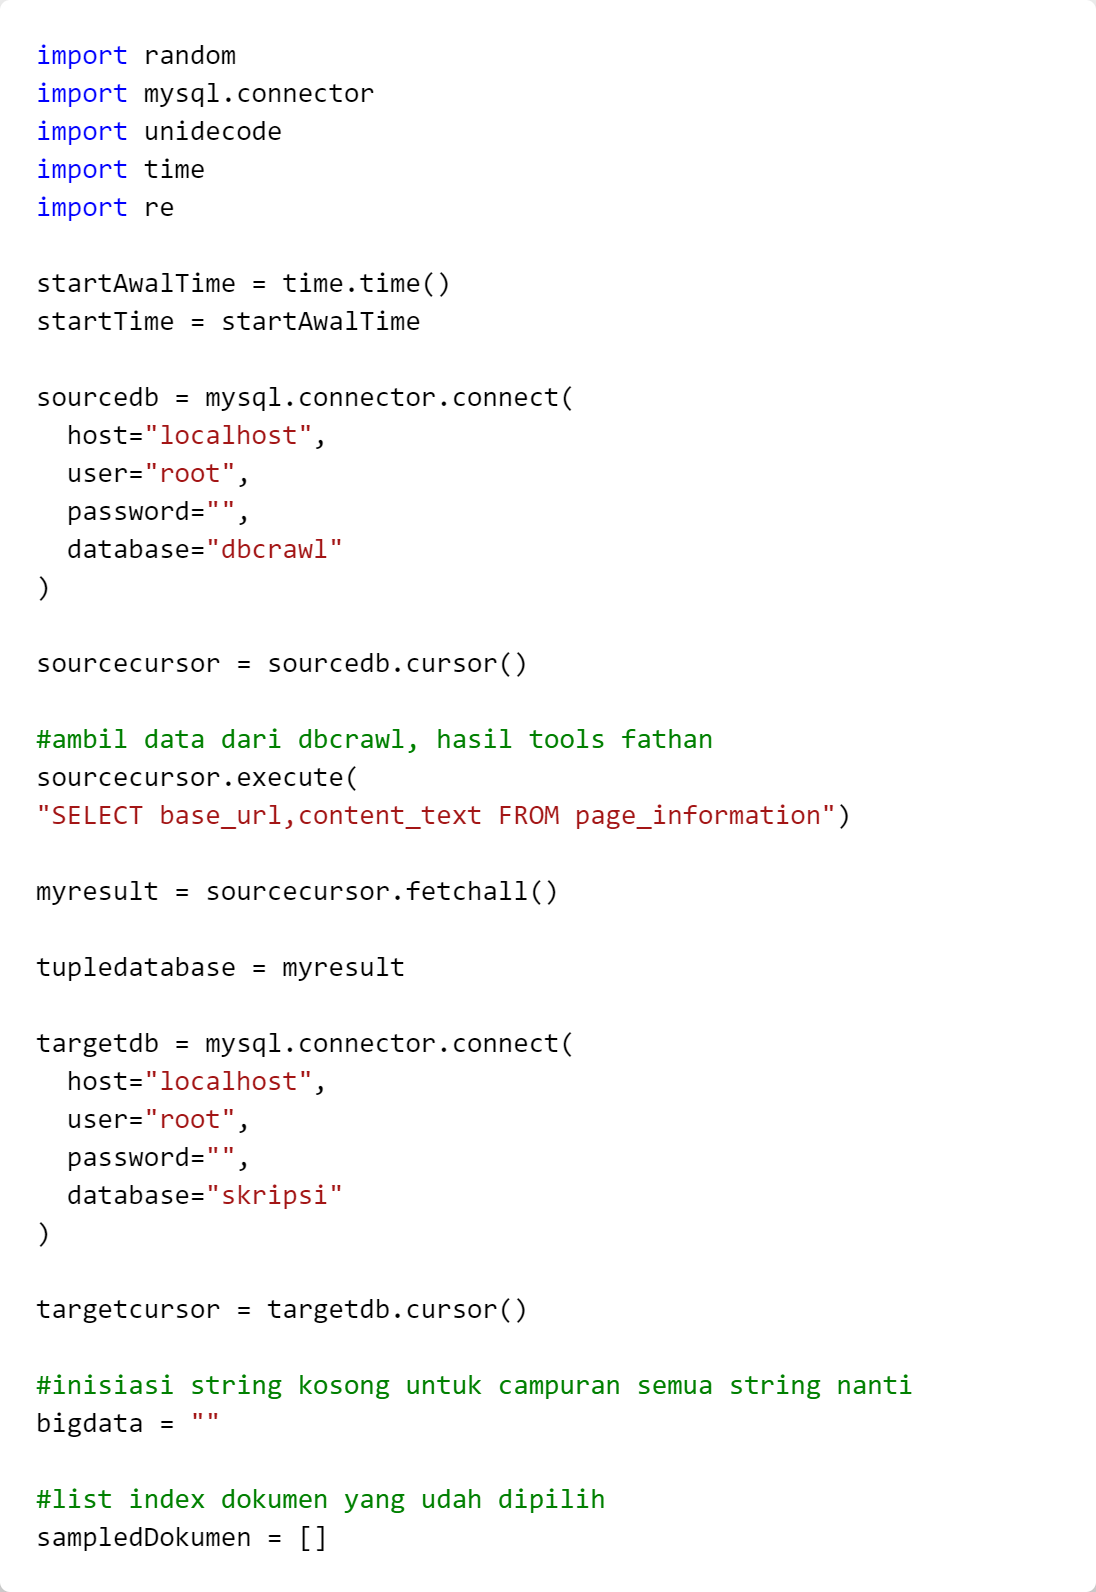
\includegraphics[scale=0.3]{onehotencode1}
\end{figure}
\begin{figure}[H]
\centering
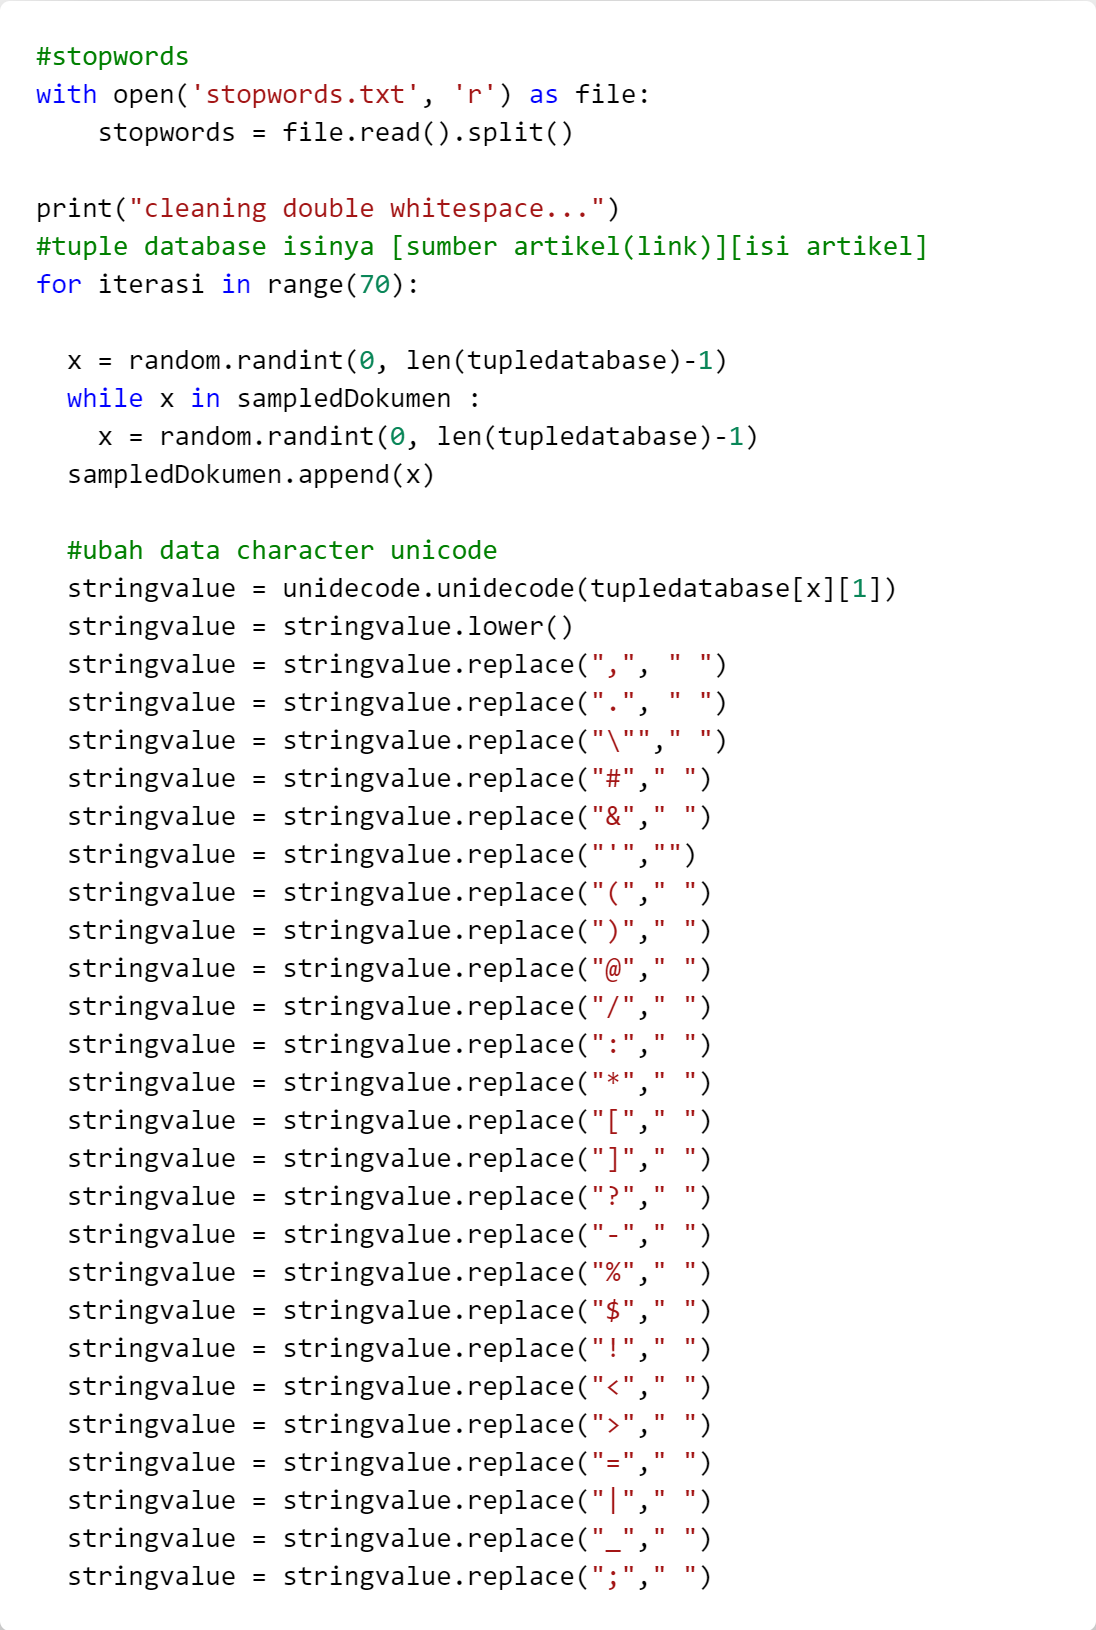
\includegraphics[scale=0.3]{onehotencode2}
\end{figure}
\begin{figure}[H]
\centering
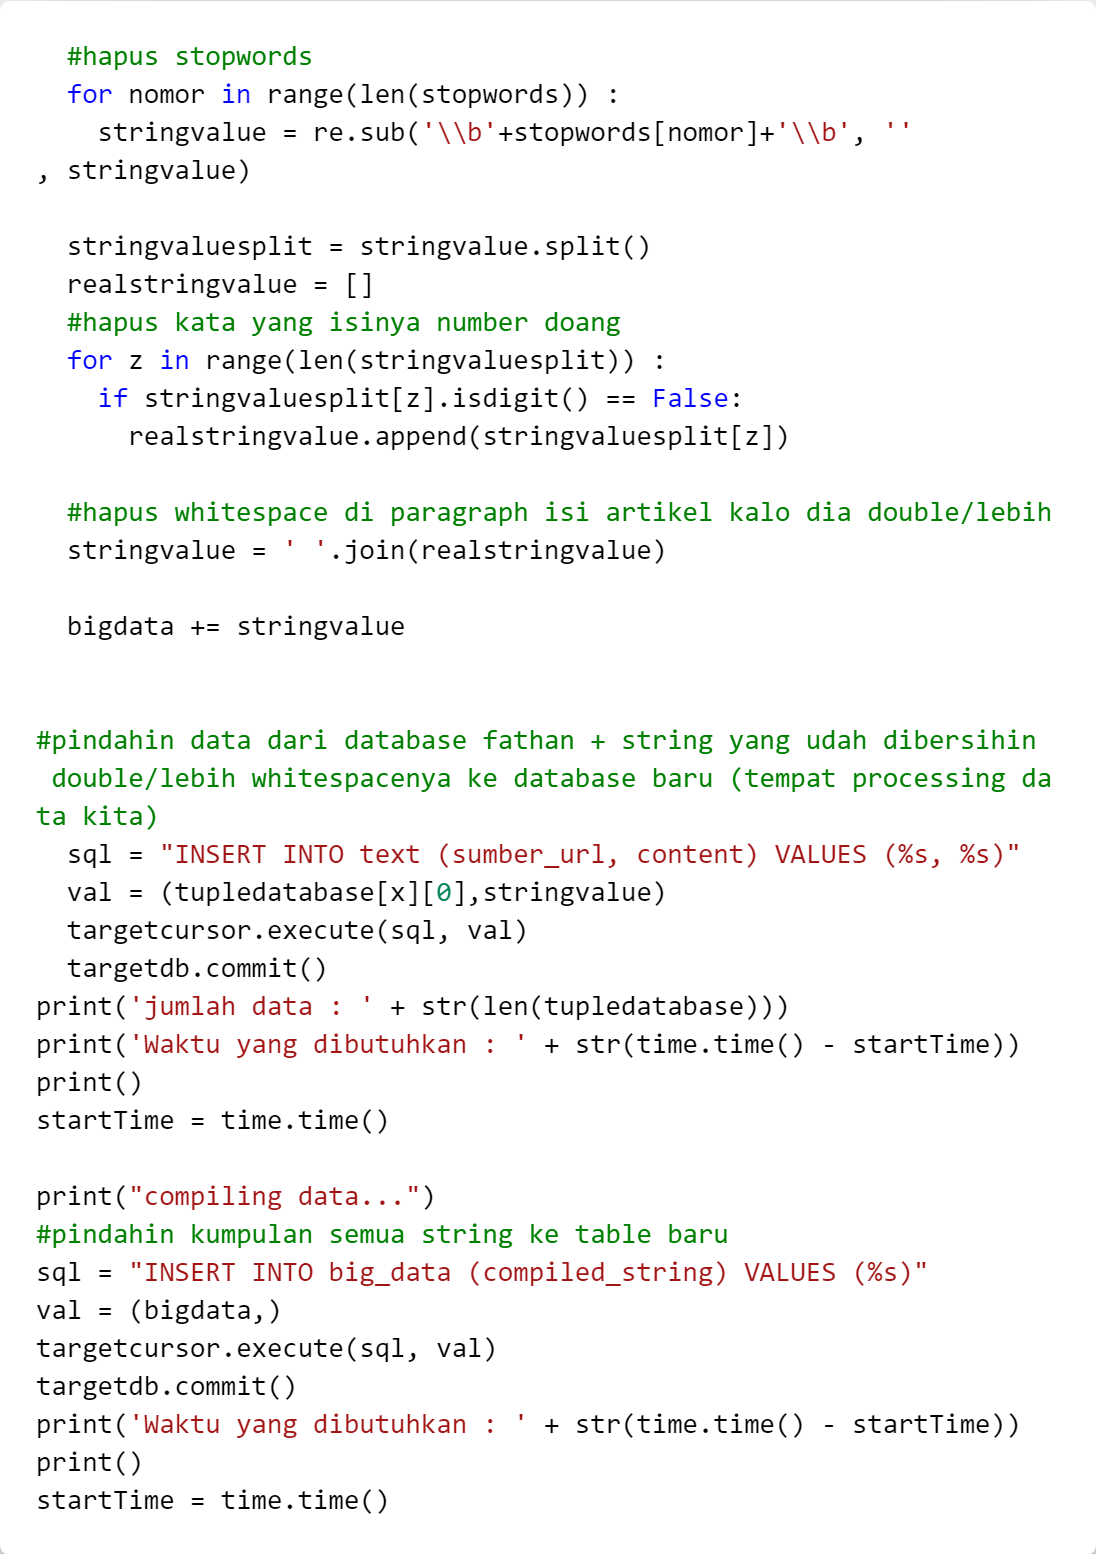
\includegraphics[scale=0.3]{onehotencode3}
\end{figure}
\begin{figure}[H]
\centering
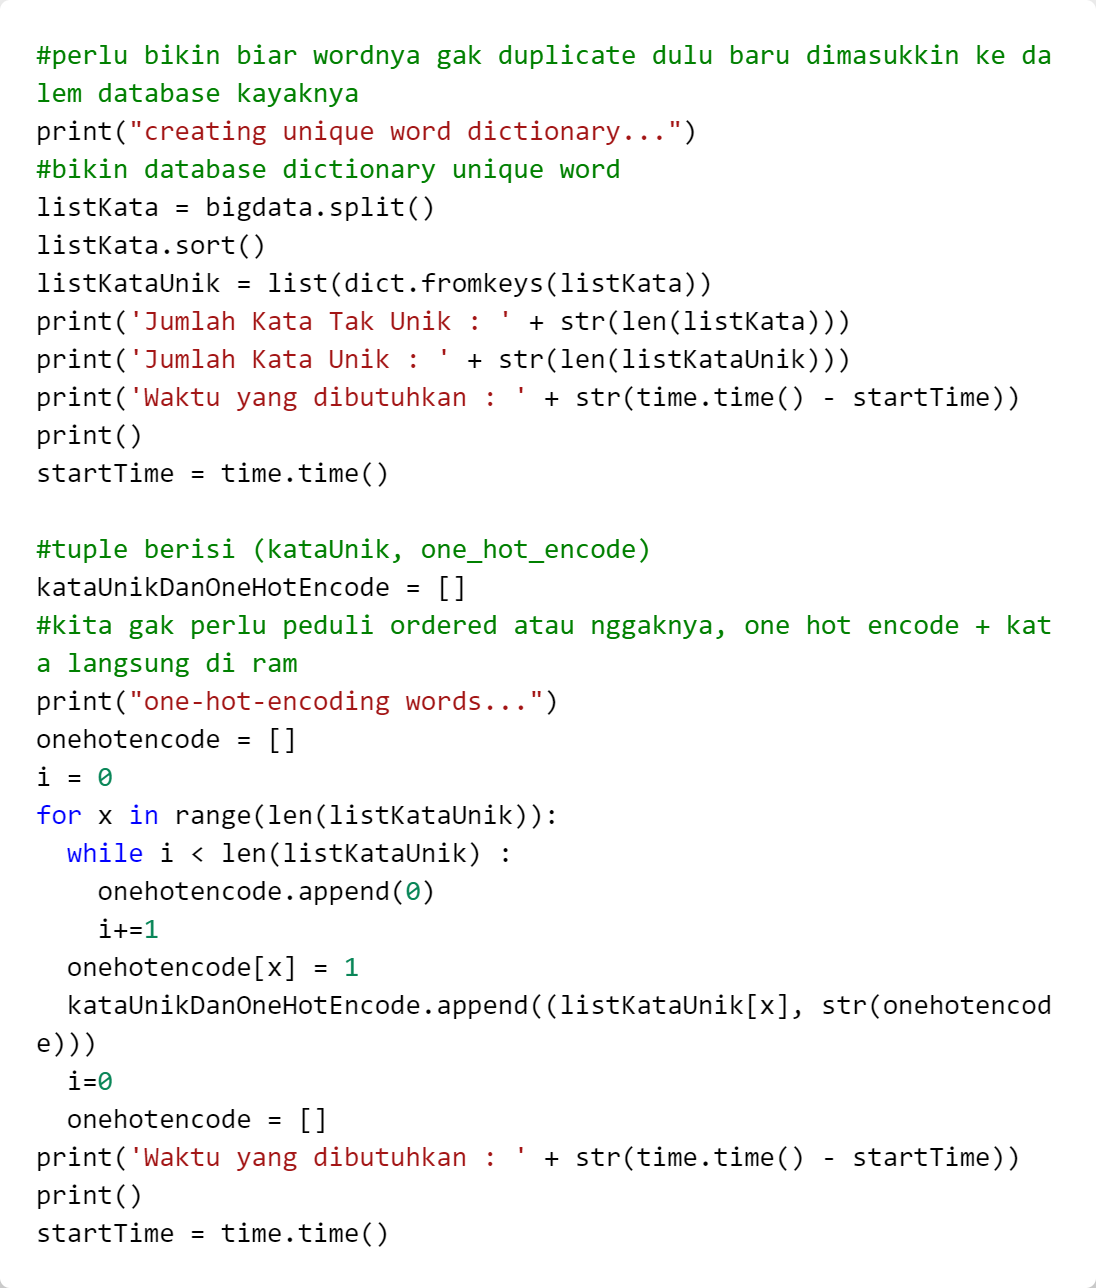
\includegraphics[scale=0.3]{onehotencode4}
\end{figure}
\begin{figure}[H]
\centering
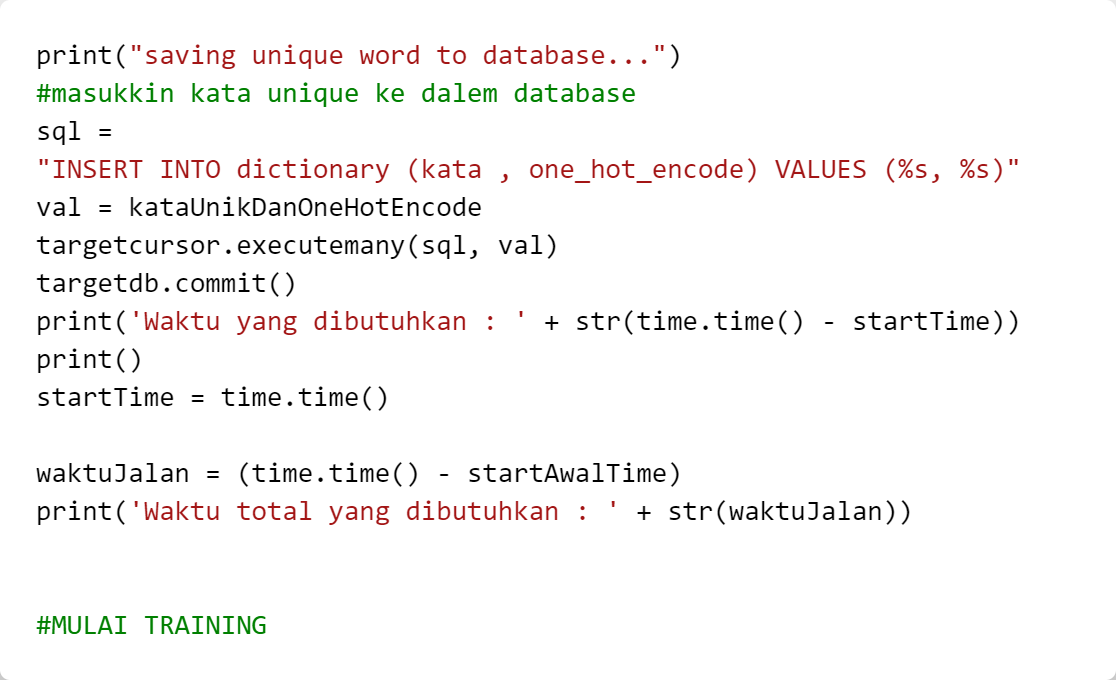
\includegraphics[scale=0.3]{onehotencode5}
\end{figure}

\newpage
{\parindent0pt \textbf{Lampiran 3 \textit{Source Code} training.py}}
\begin{figure}[H]
\centering
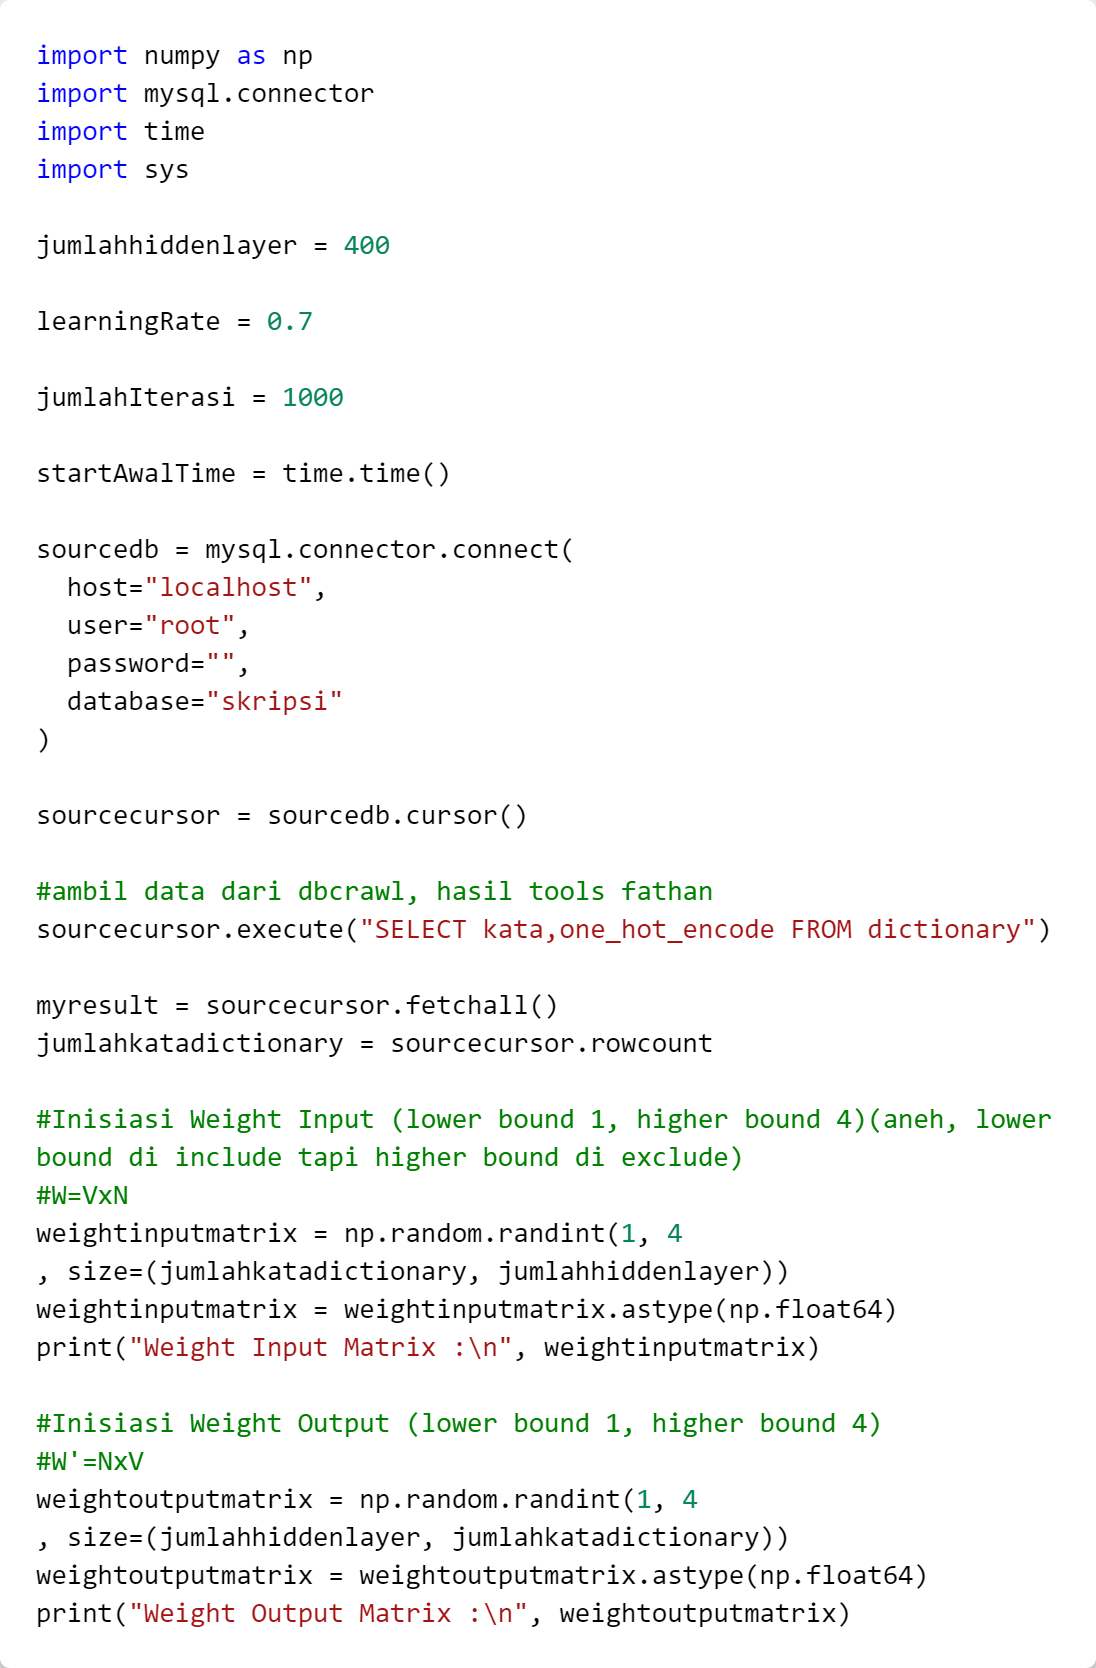
\includegraphics[scale=0.3]{training1}
\end{figure}
\begin{figure}[H]
\centering
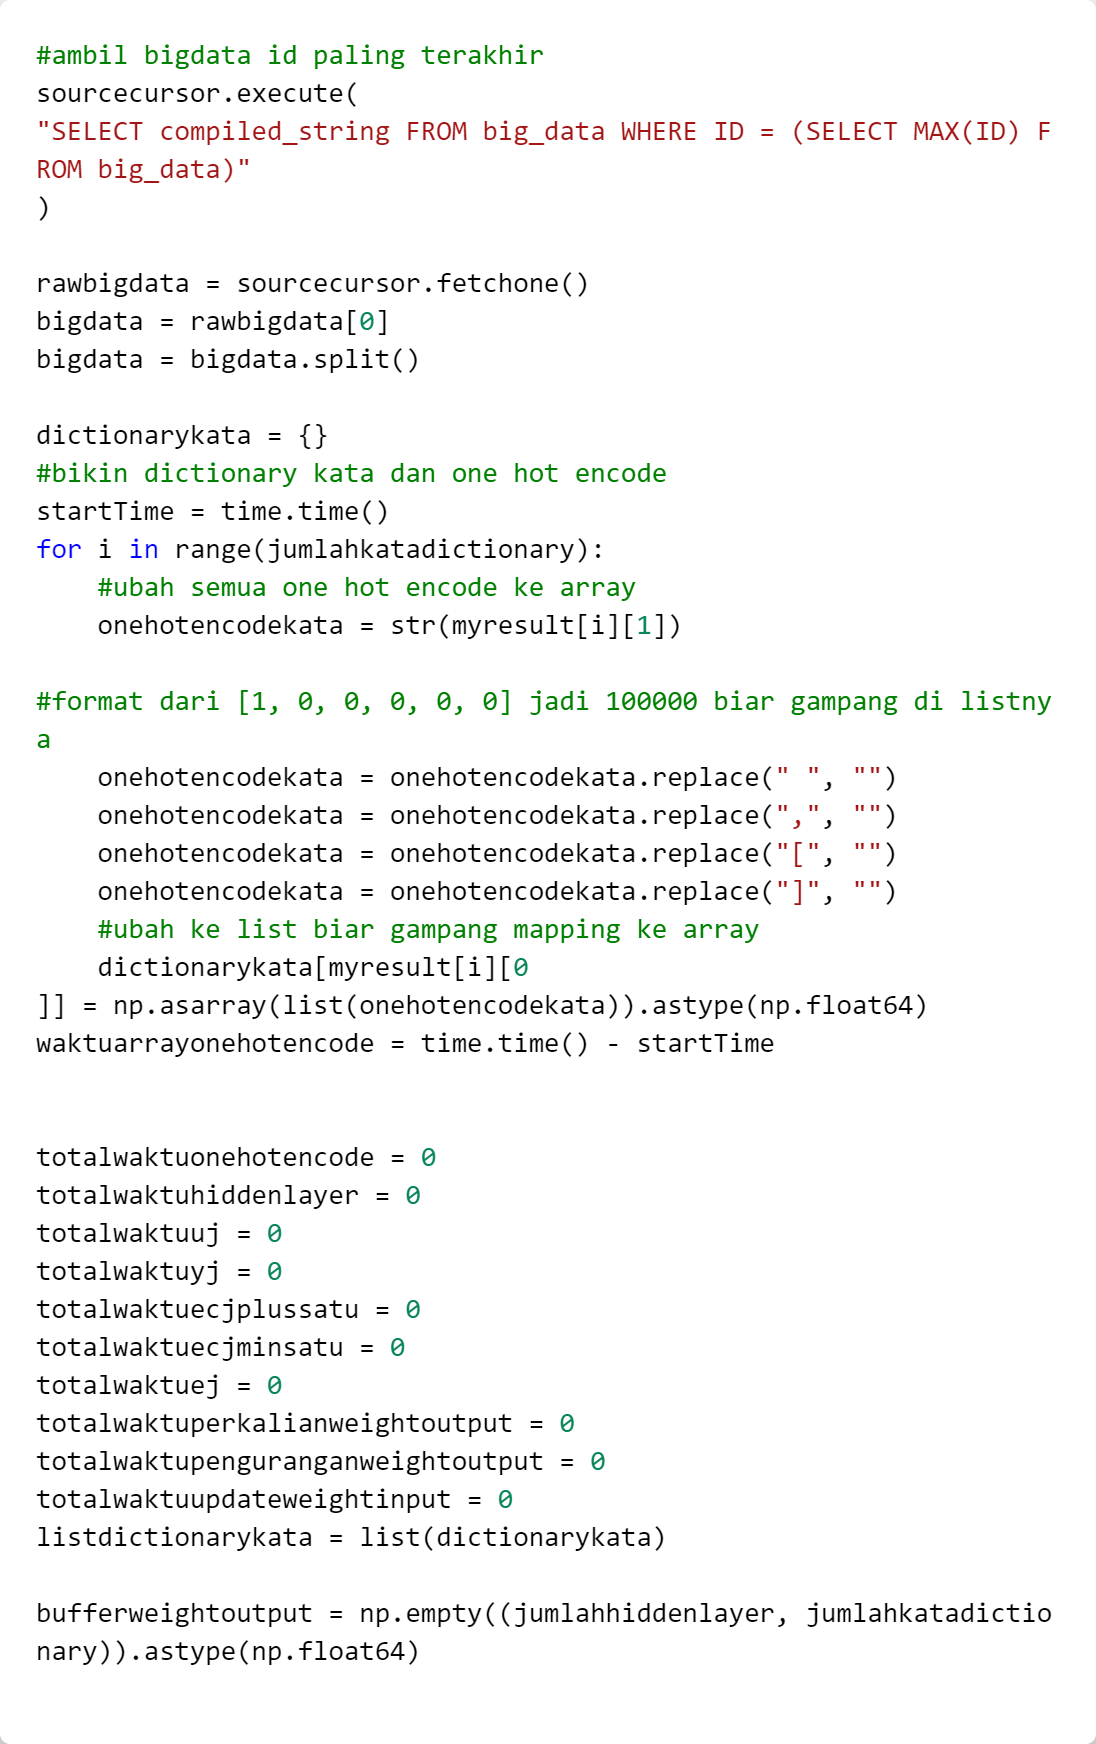
\includegraphics[scale=0.3]{training2}
\end{figure}
\begin{figure}[H]
\centering
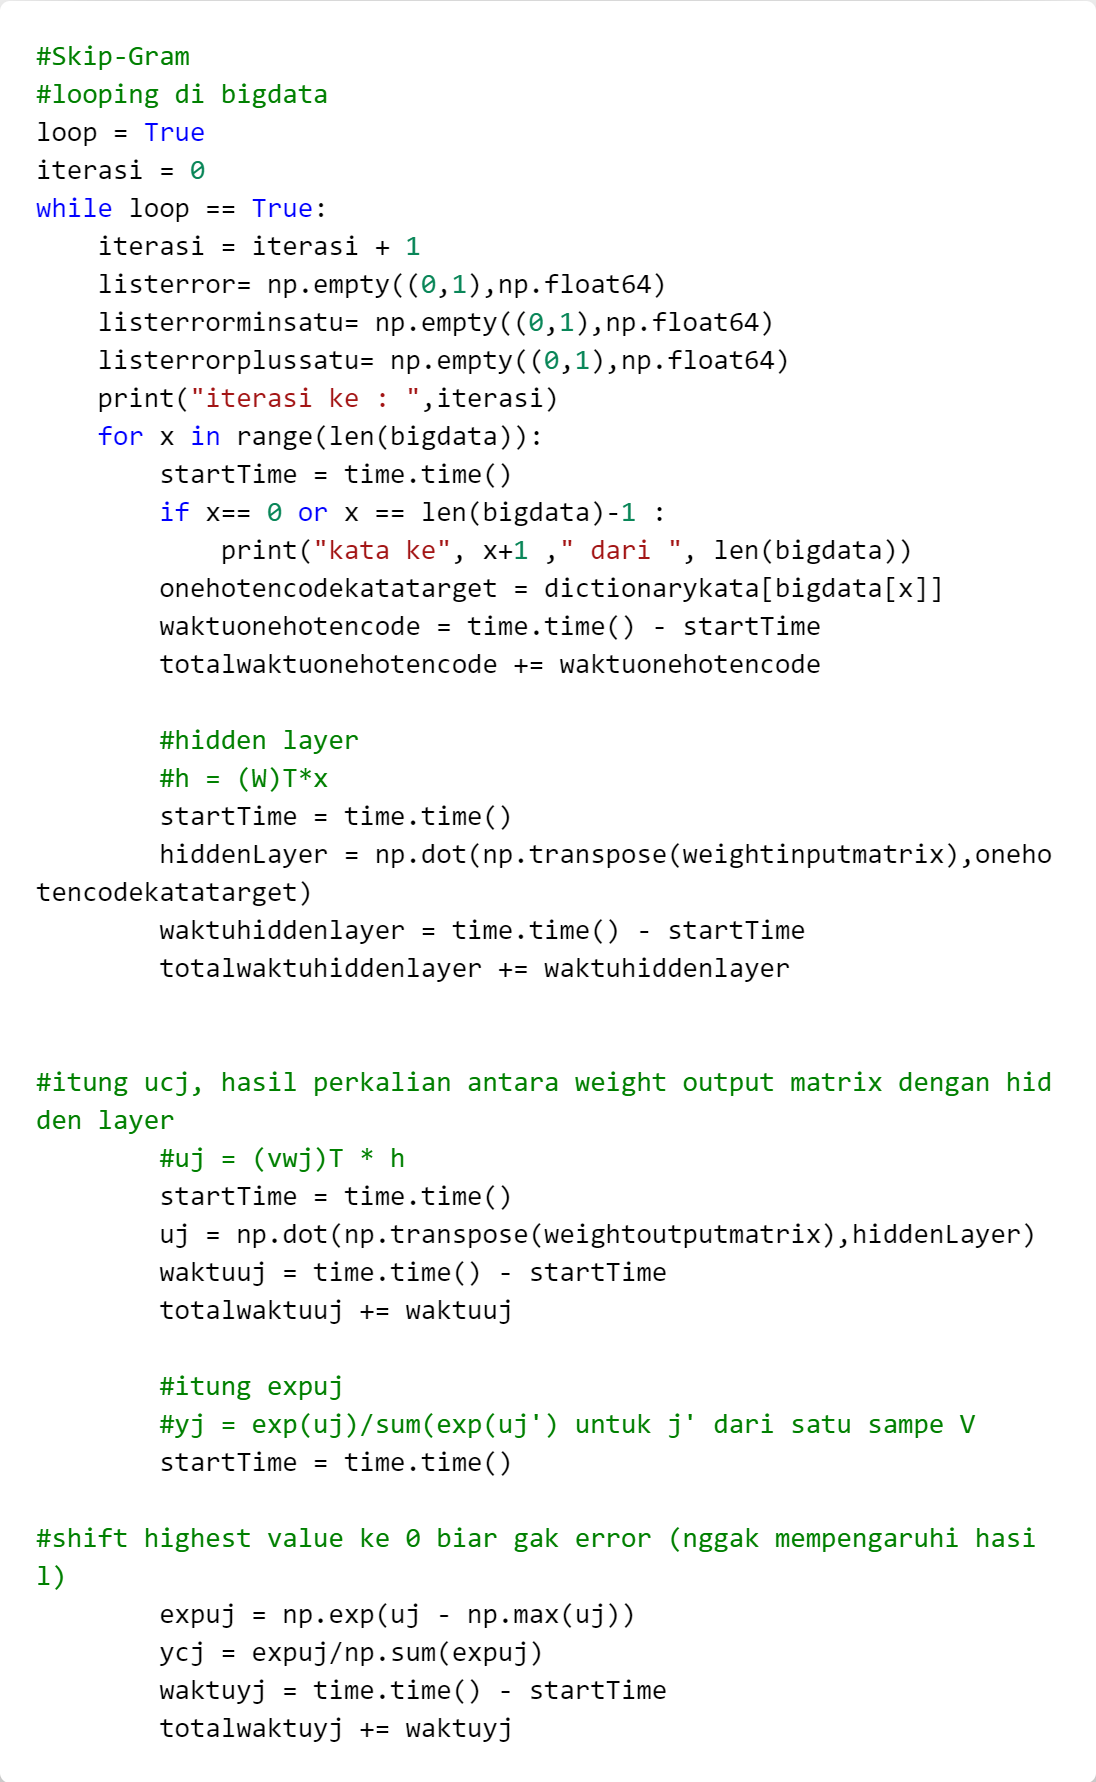
\includegraphics[scale=0.3]{training3}
\end{figure}
\begin{figure}[H]
\centering
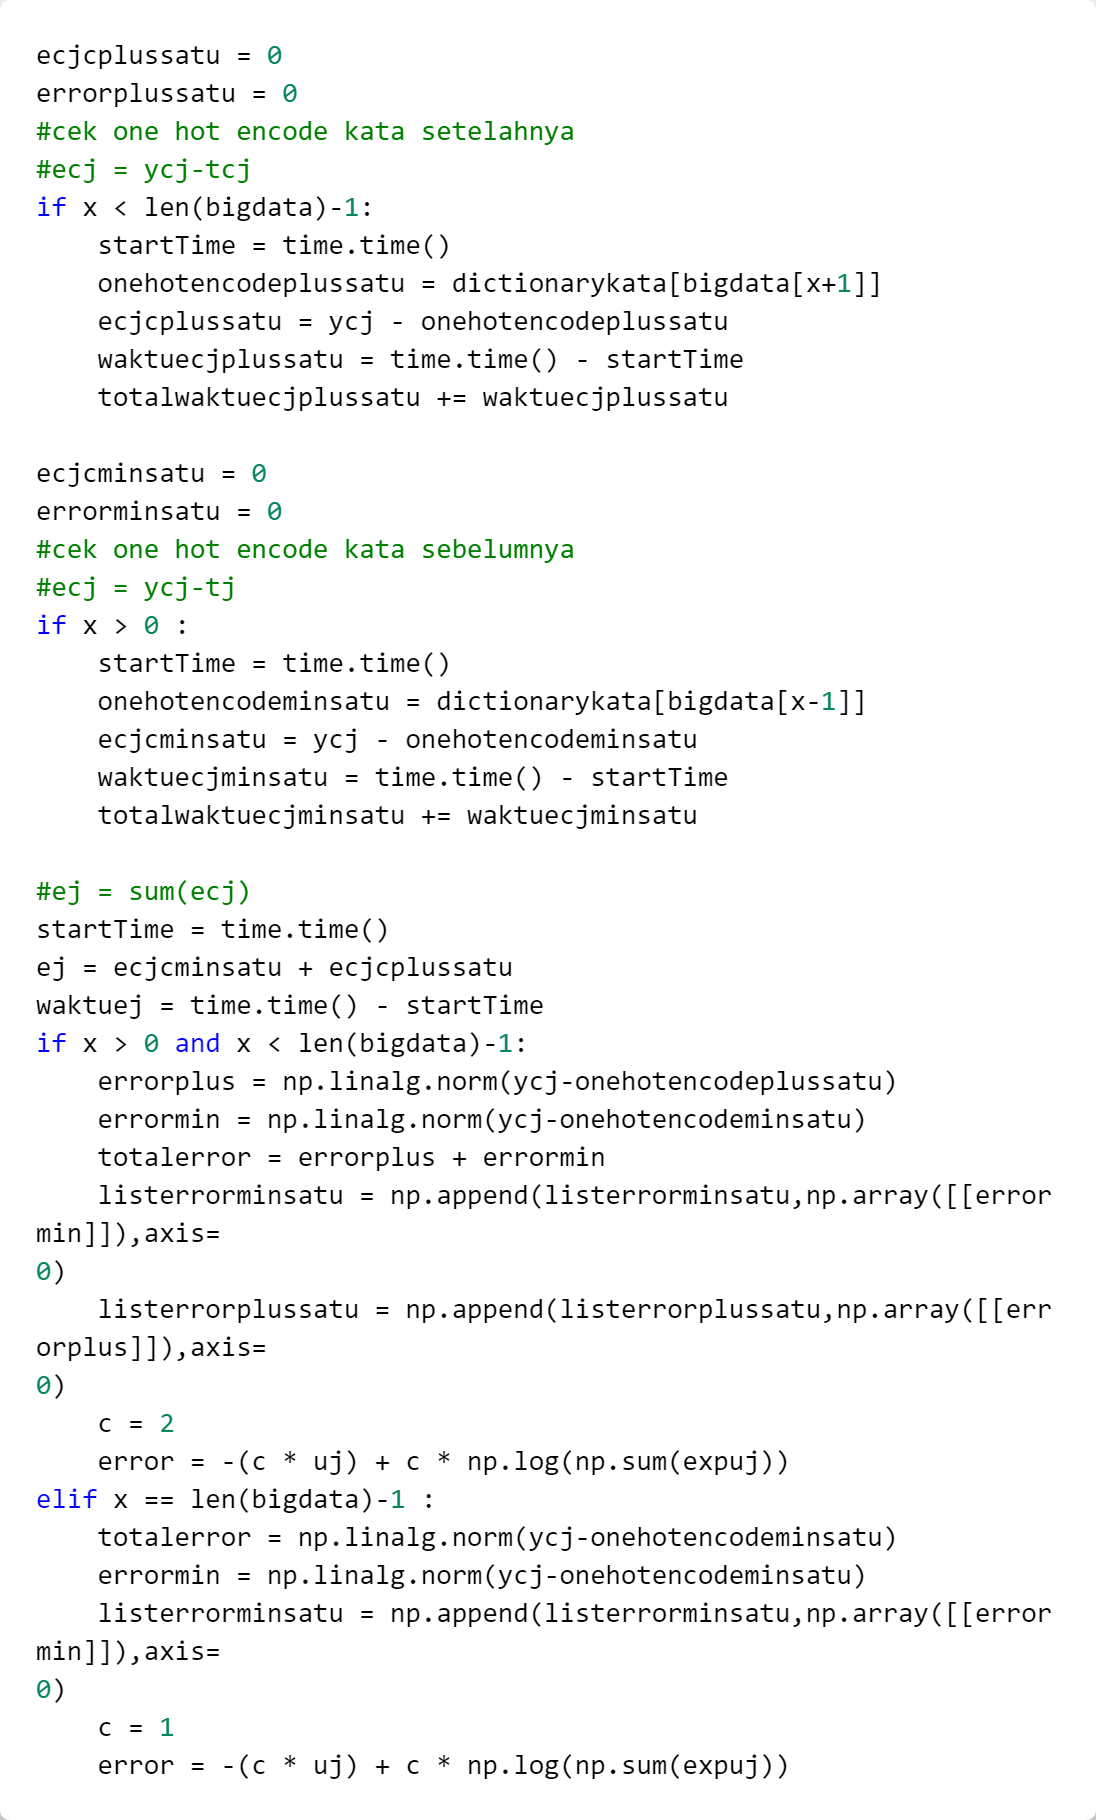
\includegraphics[scale=0.3]{training4}
\end{figure}
\begin{figure}[H]
\centering
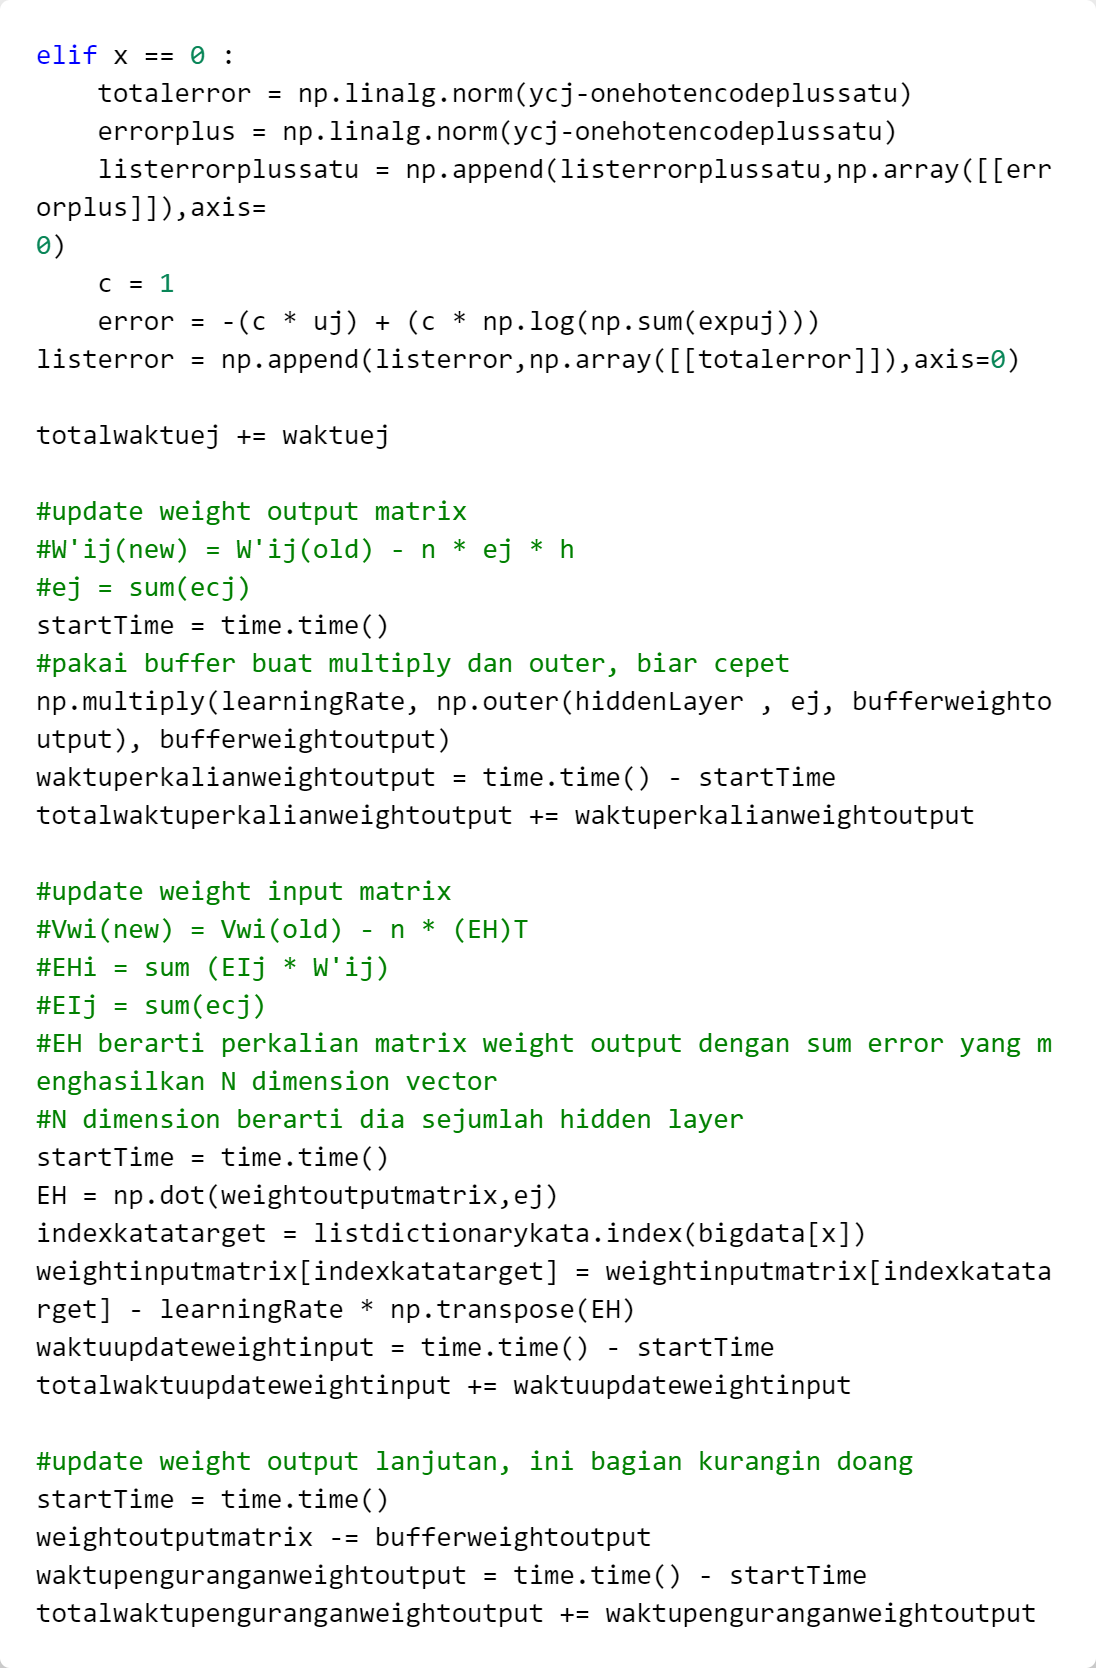
\includegraphics[scale=0.3]{training5}
\end{figure}
\begin{figure}[H]
\centering
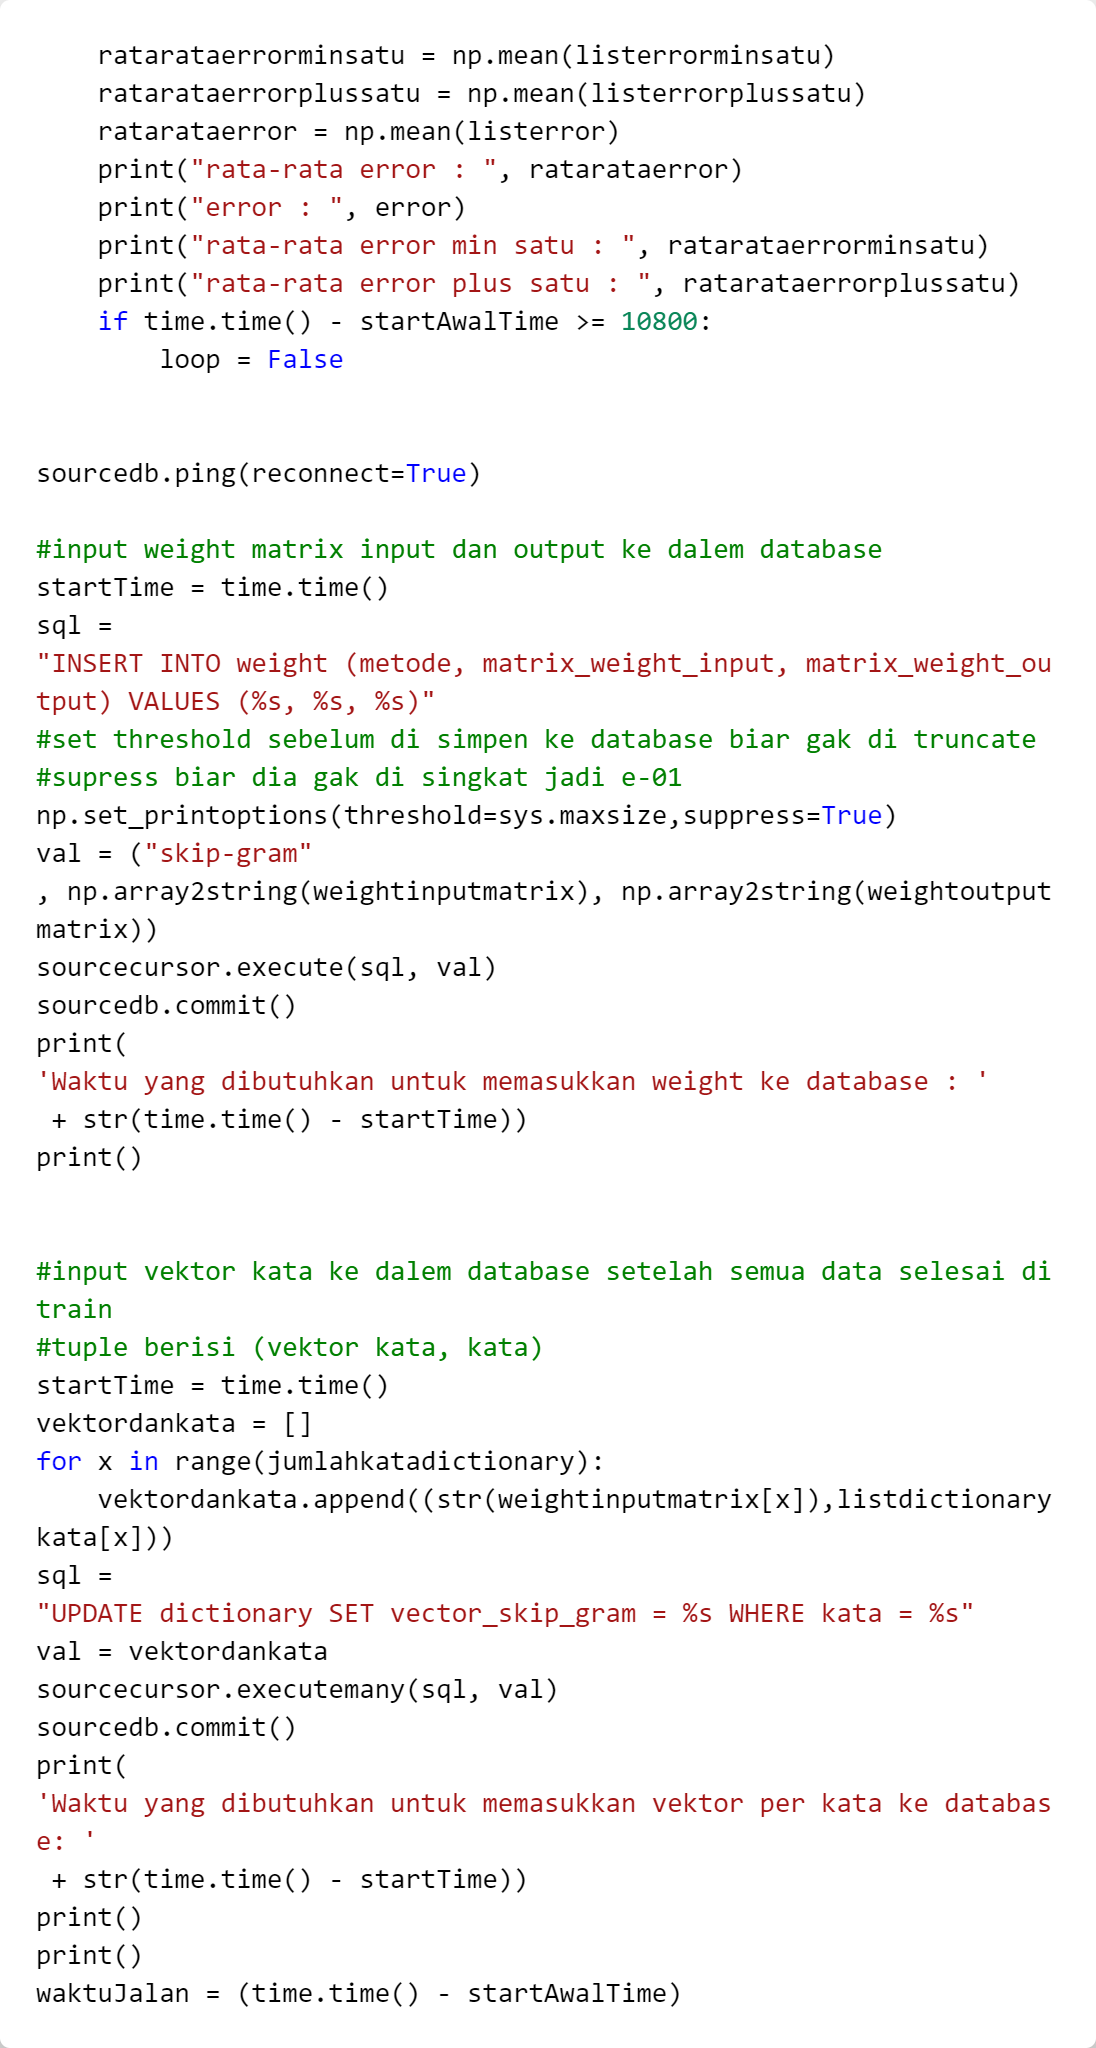
\includegraphics[scale=0.3]{training6}
\end{figure}
\begin{figure}[H]
\centering
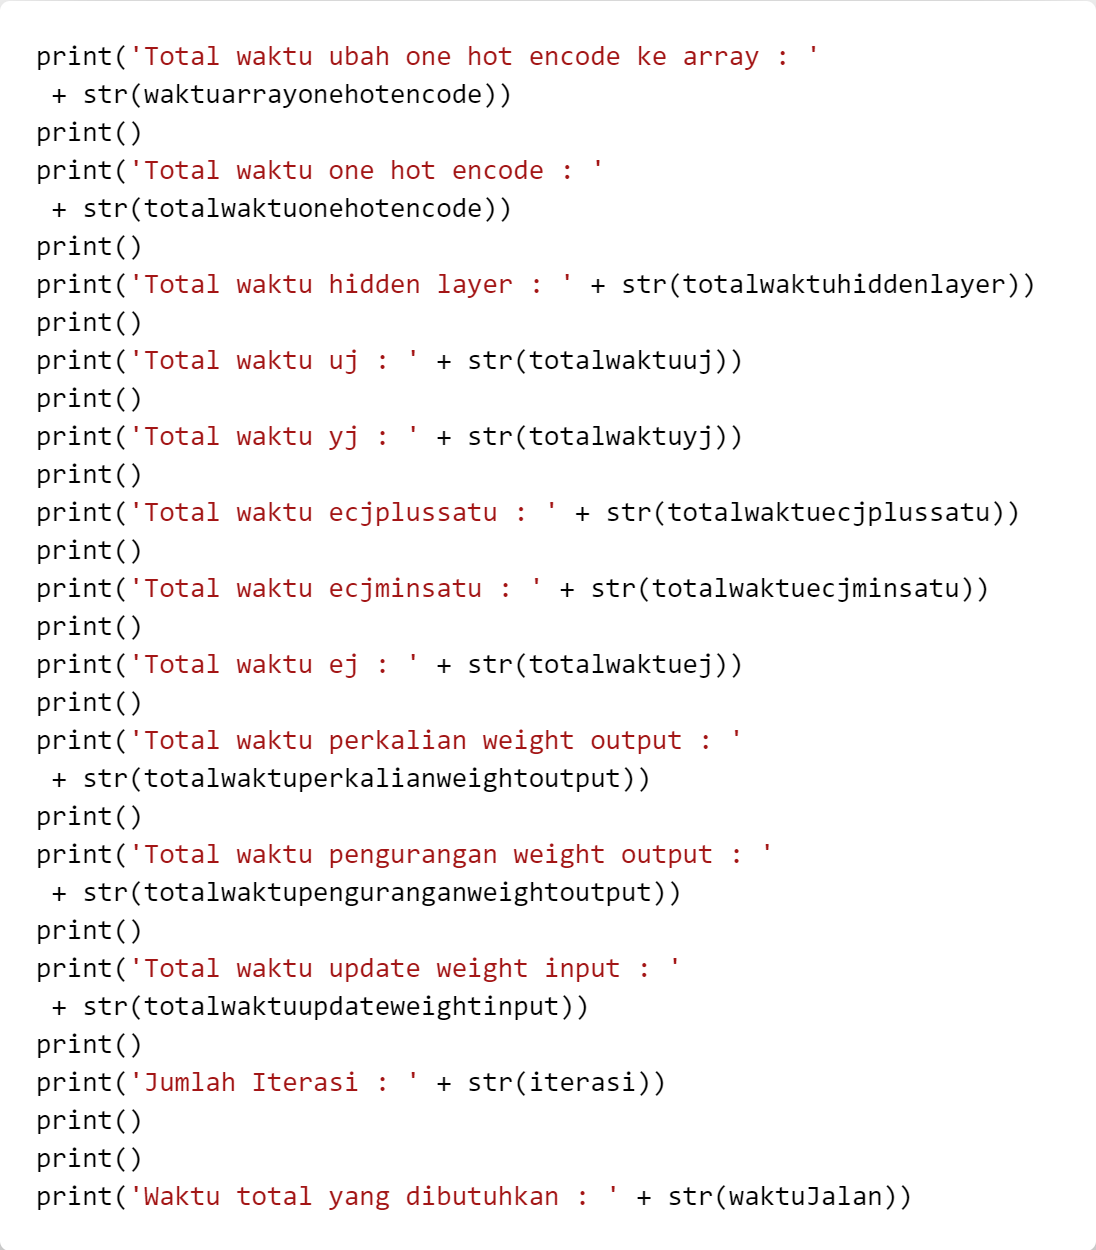
\includegraphics[scale=0.3]{training7}
\end{figure}

\newpage
{\parindent0pt \textbf{Lampiran 4 \textit{Source Code} trainingcbow.py}}
\begin{figure}[H]
\centering
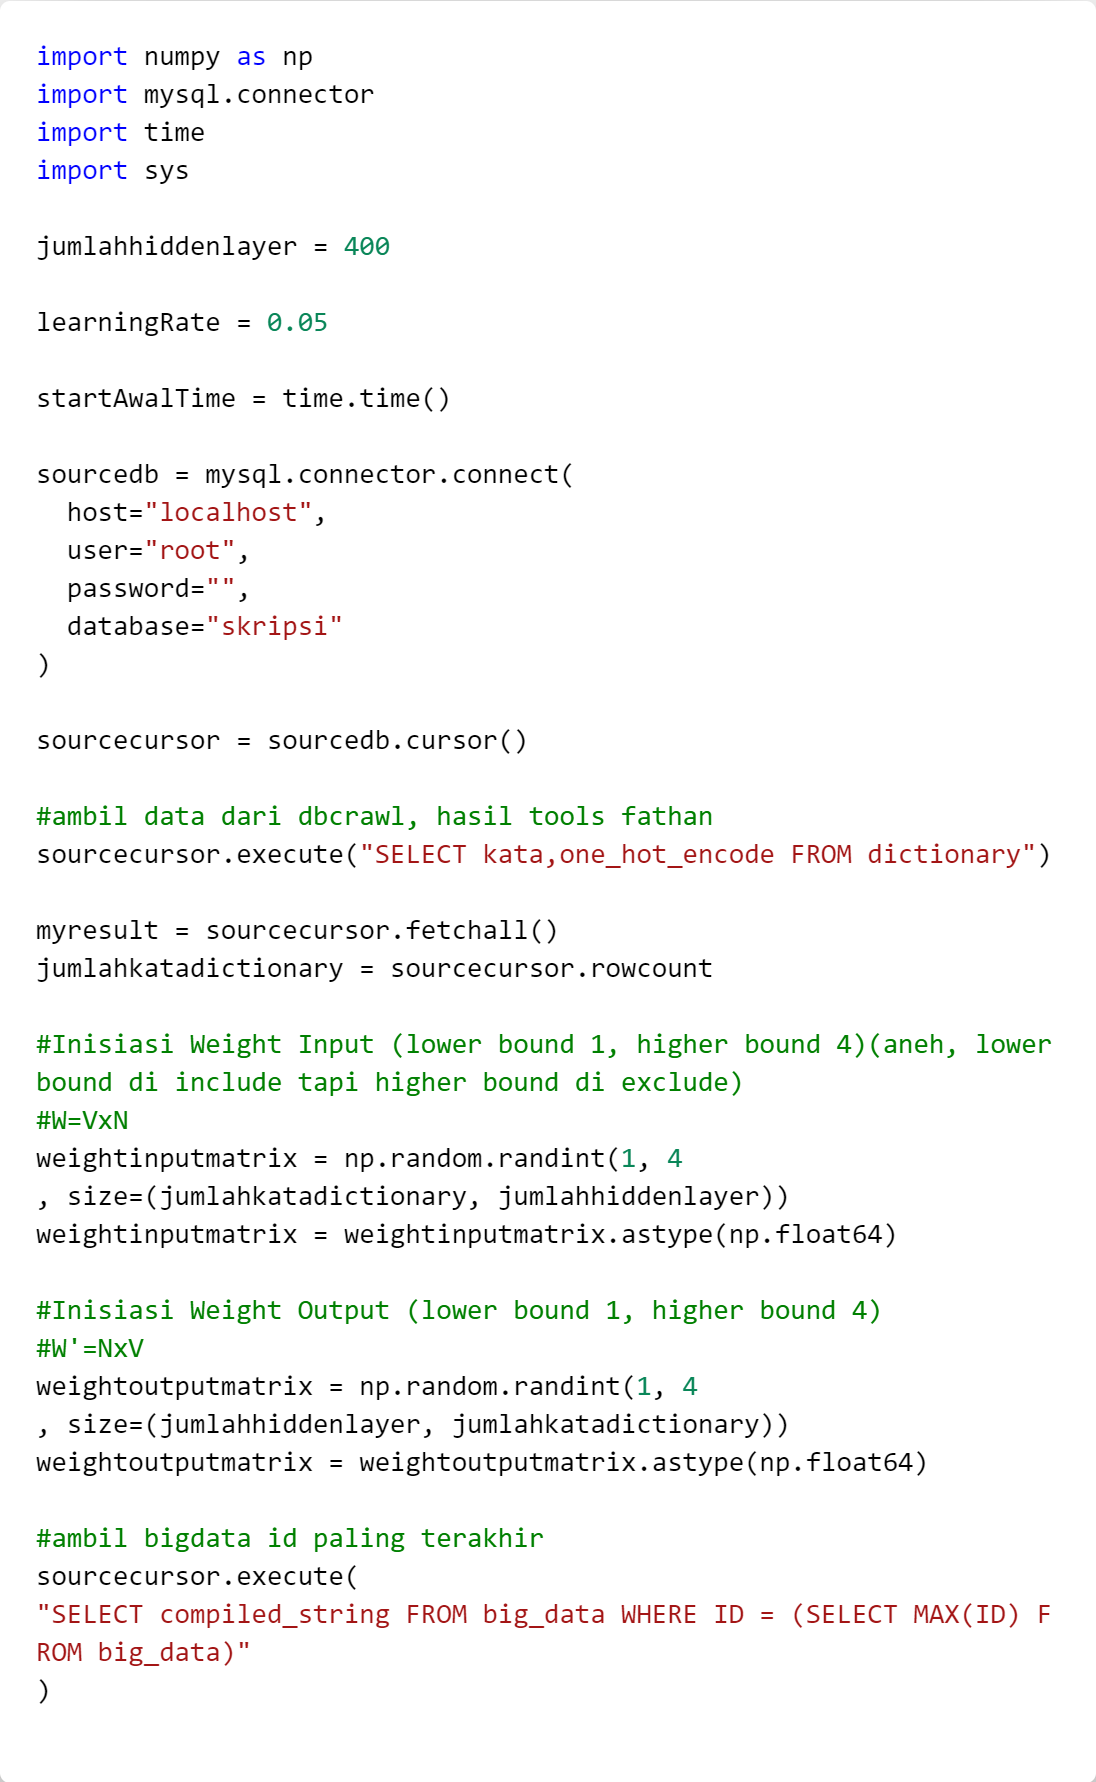
\includegraphics[scale=0.3]{trainingcbow1}
\end{figure}
\begin{figure}[H]
\centering
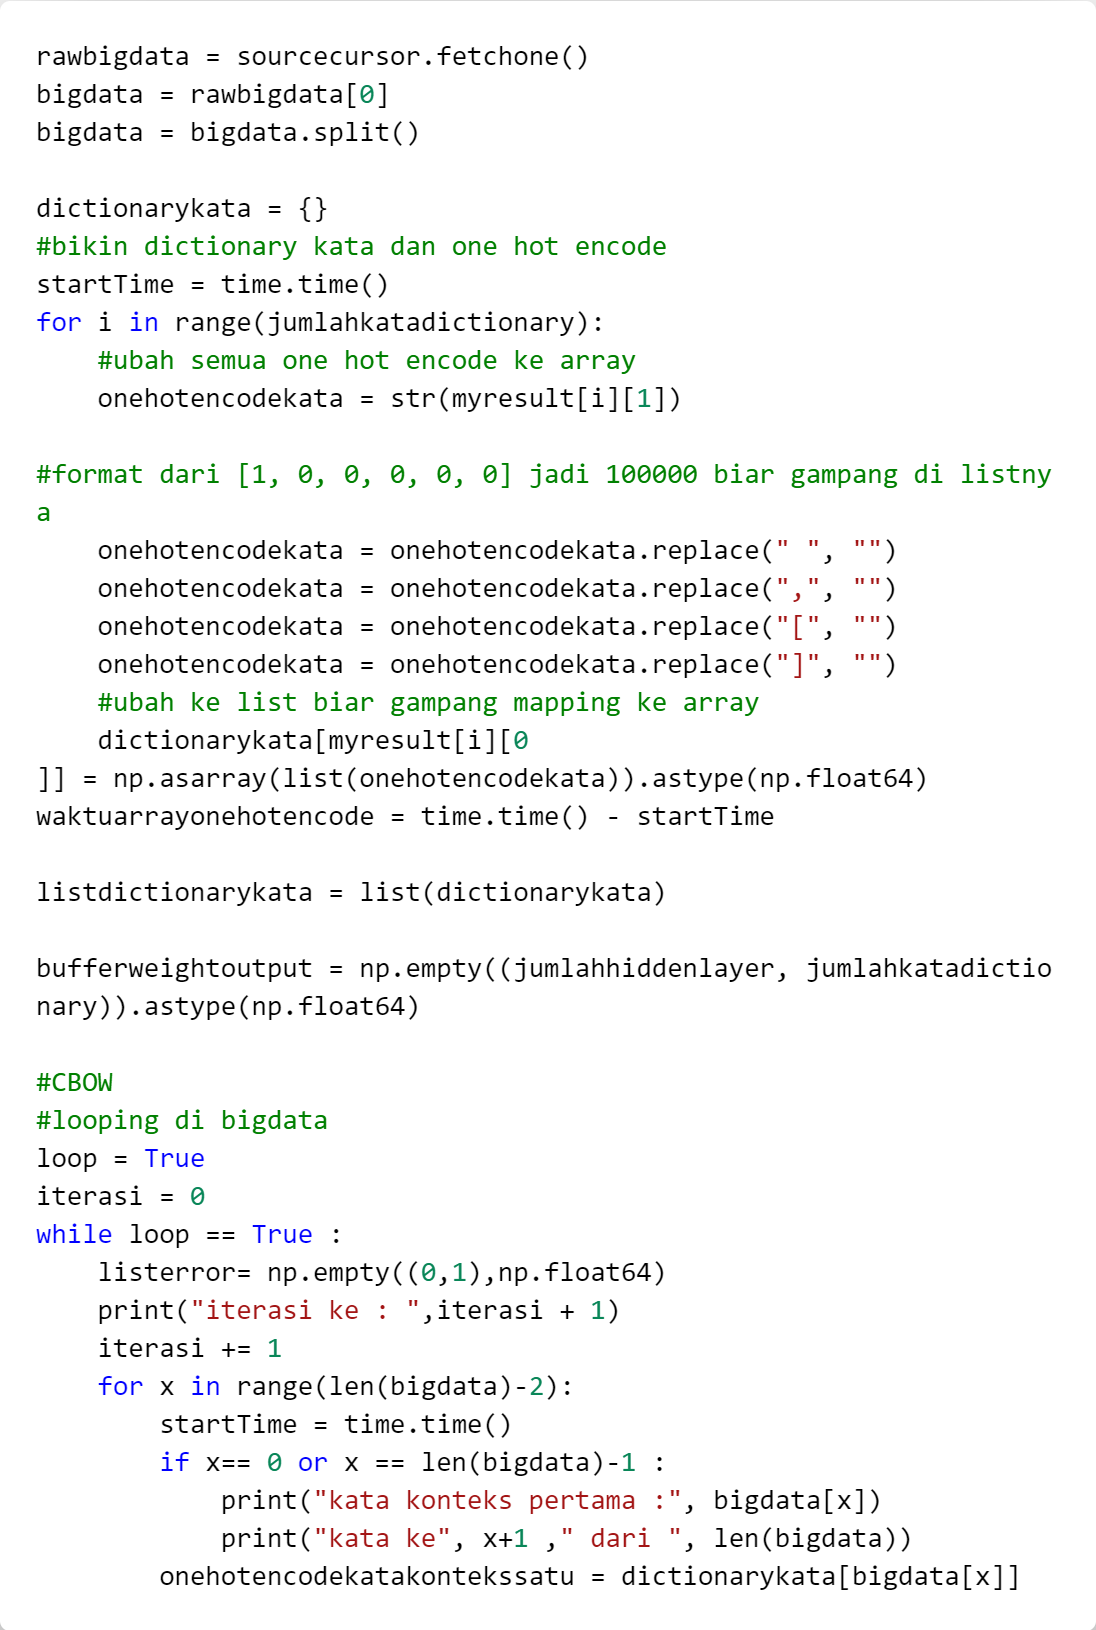
\includegraphics[scale=0.3]{trainingcbow2}
\end{figure}
\begin{figure}[H]
\centering
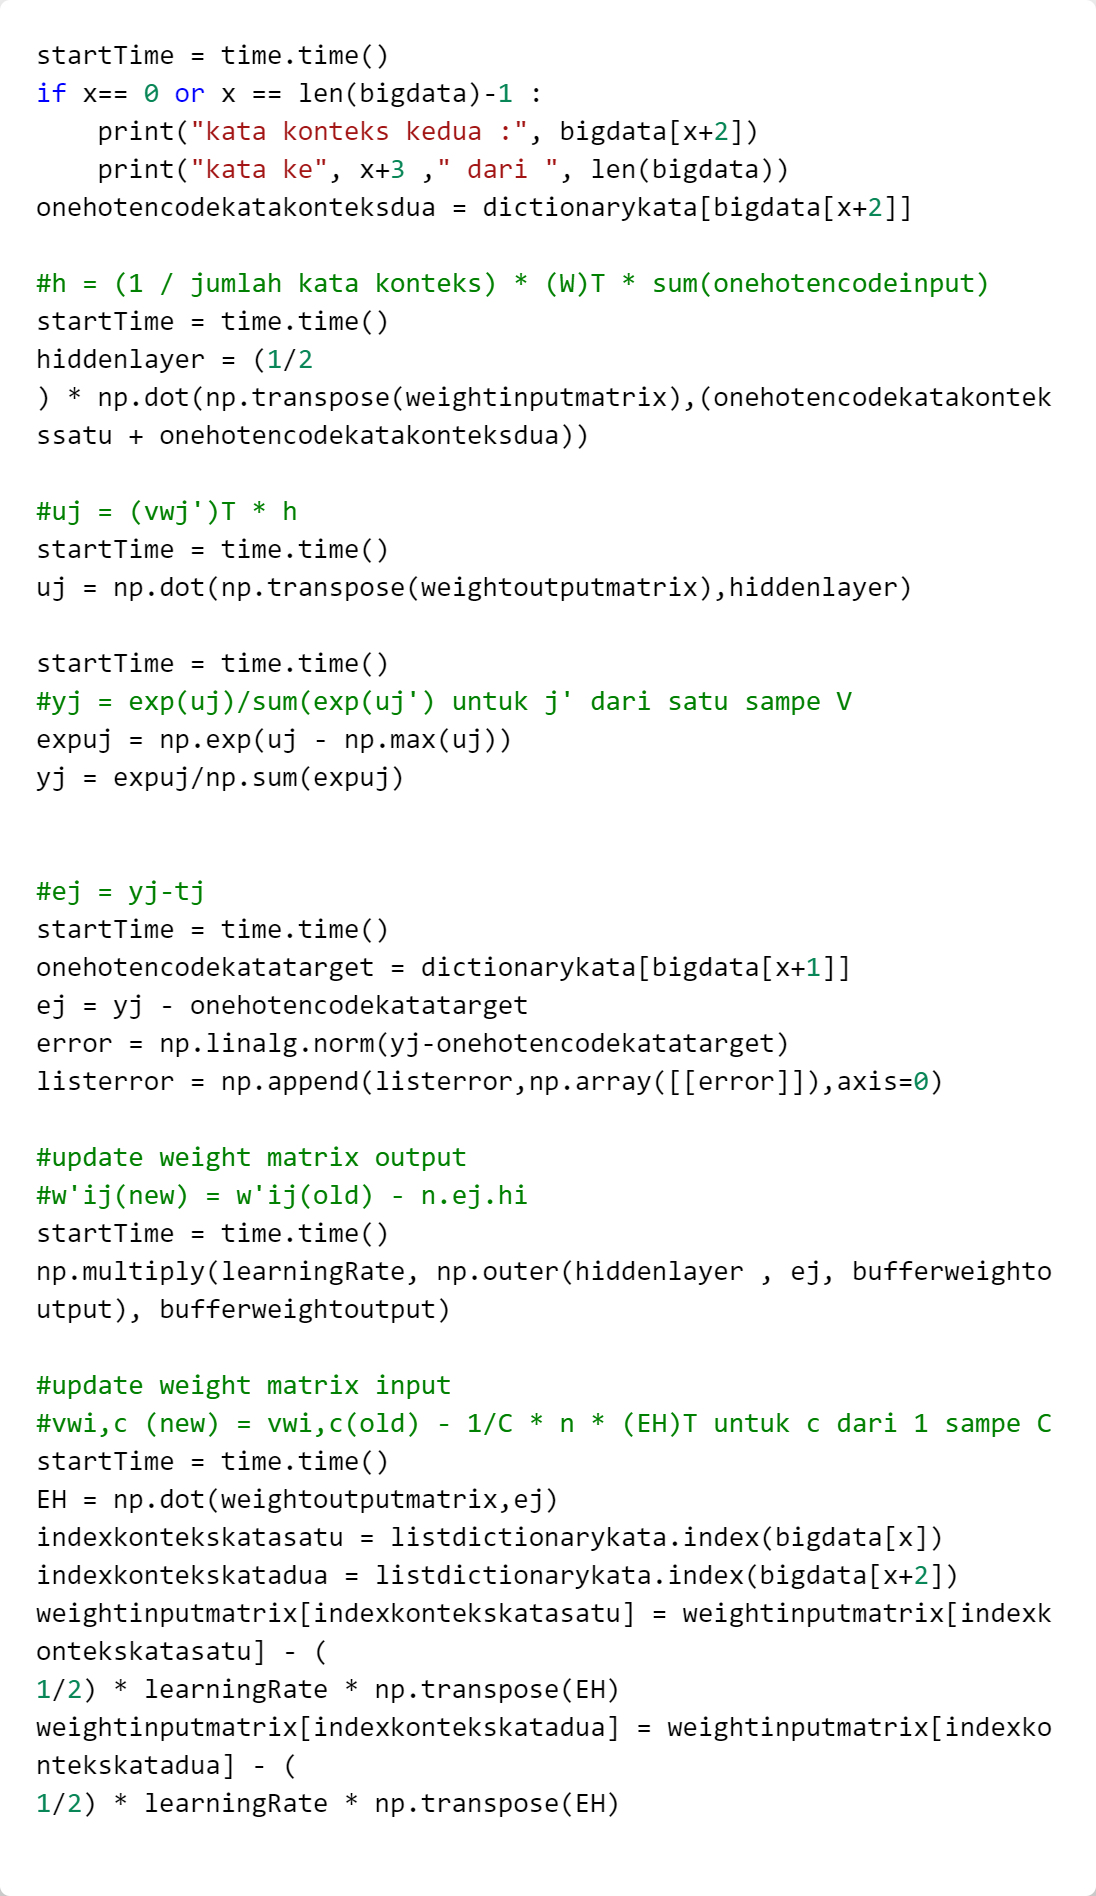
\includegraphics[scale=0.3]{trainingcbow3}
\end{figure}
\begin{figure}[H]
\centering
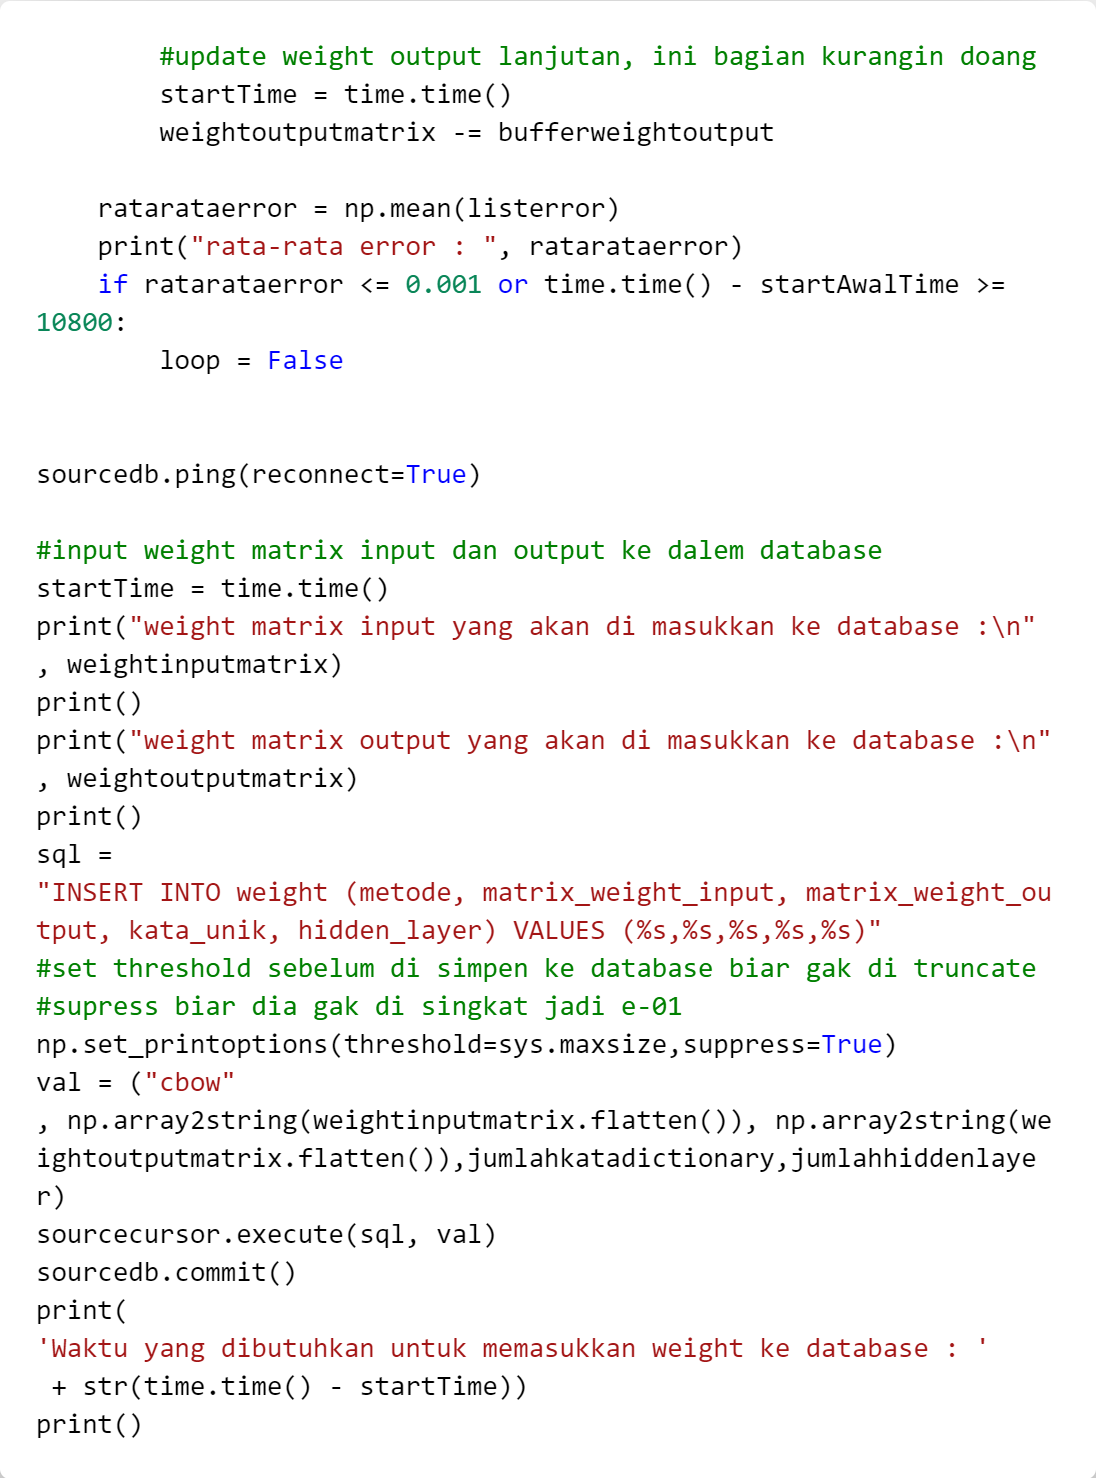
\includegraphics[scale=0.3]{trainingcbow4}
\end{figure}
\begin{figure}[H]
\centering
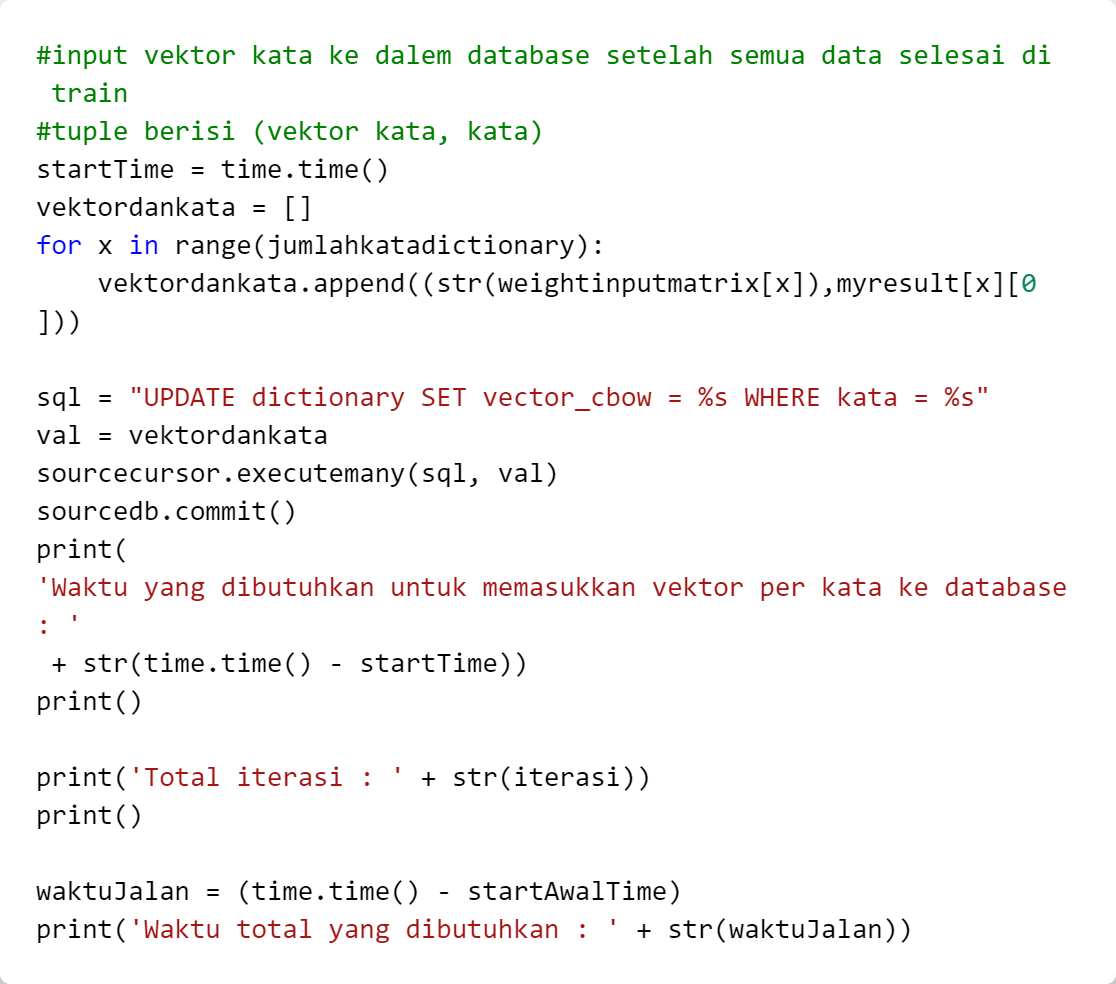
\includegraphics[scale=0.3]{trainingcbow5}
\end{figure}

\newpage
{\parindent0pt \textbf{Lampiran 5 \textit{Source Code} trainingcbow4kata.py}}
\begin{figure}[H]
\centering
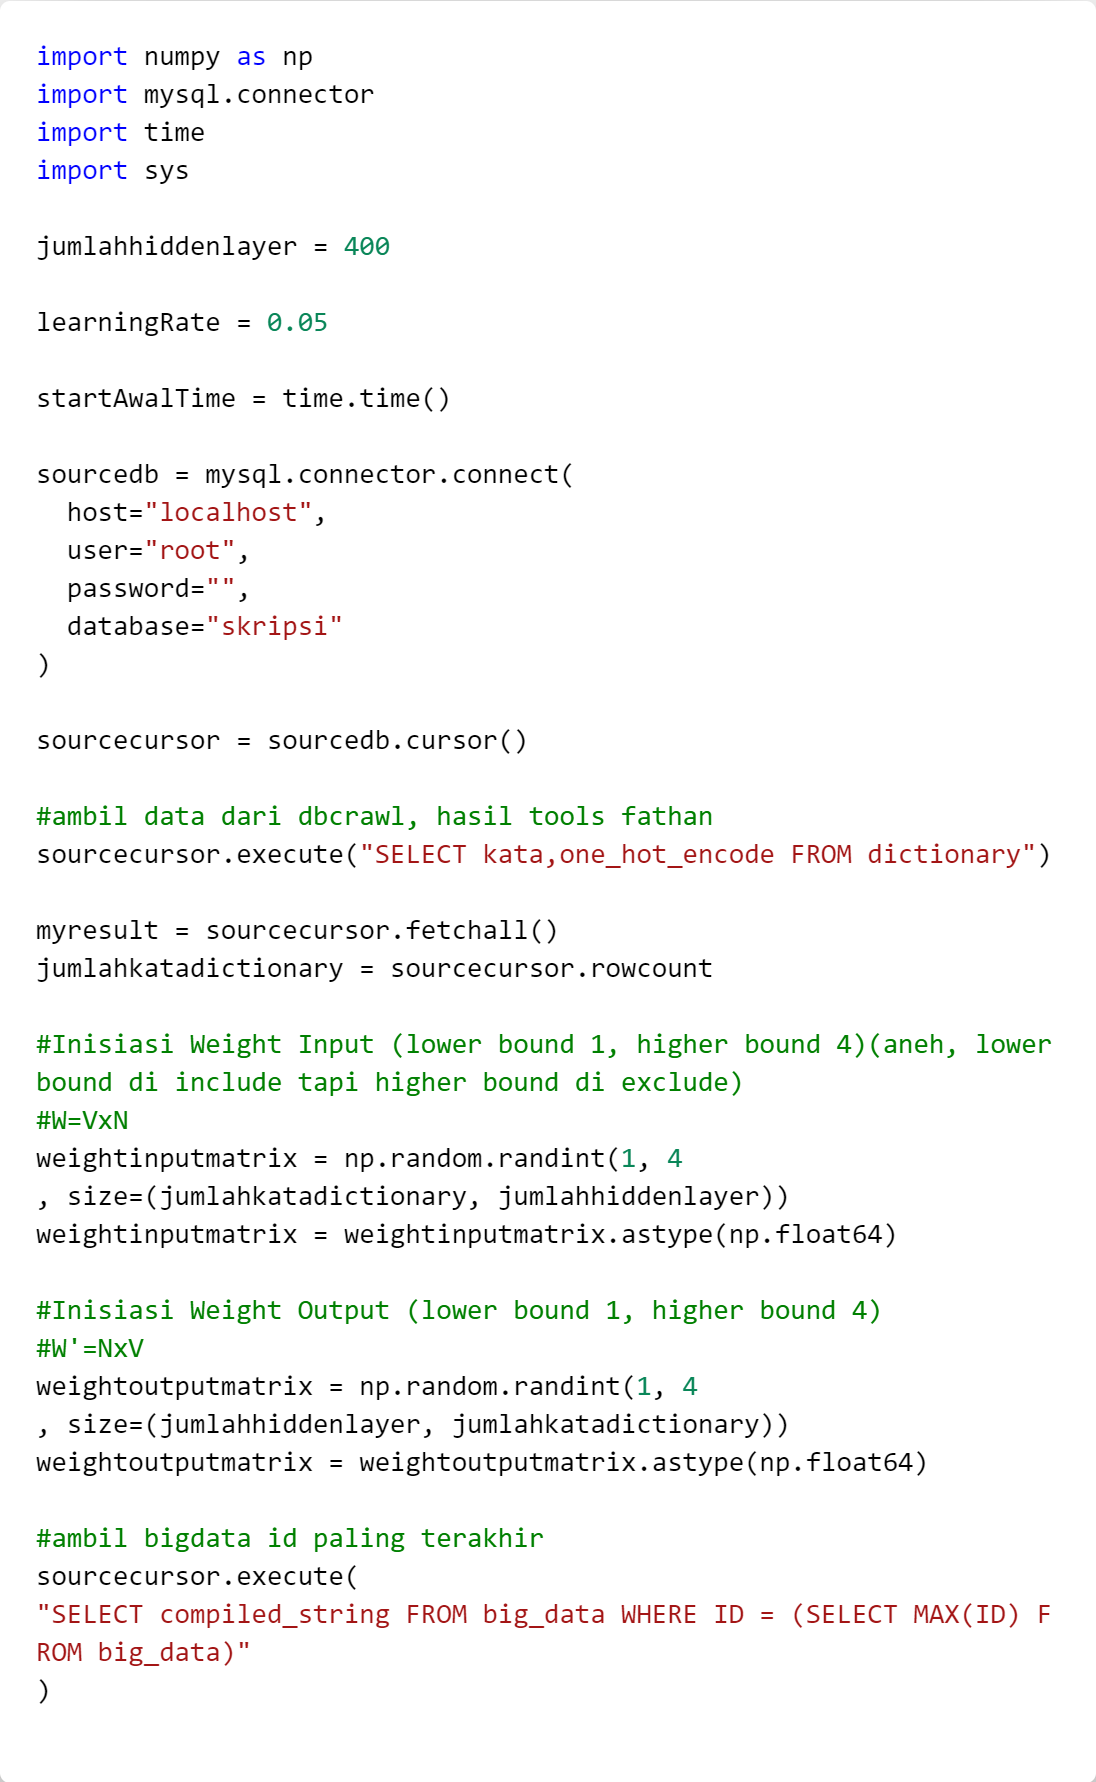
\includegraphics[scale=0.3]{trainingcbow4kata1}
\end{figure}
\begin{figure}[H]
\centering
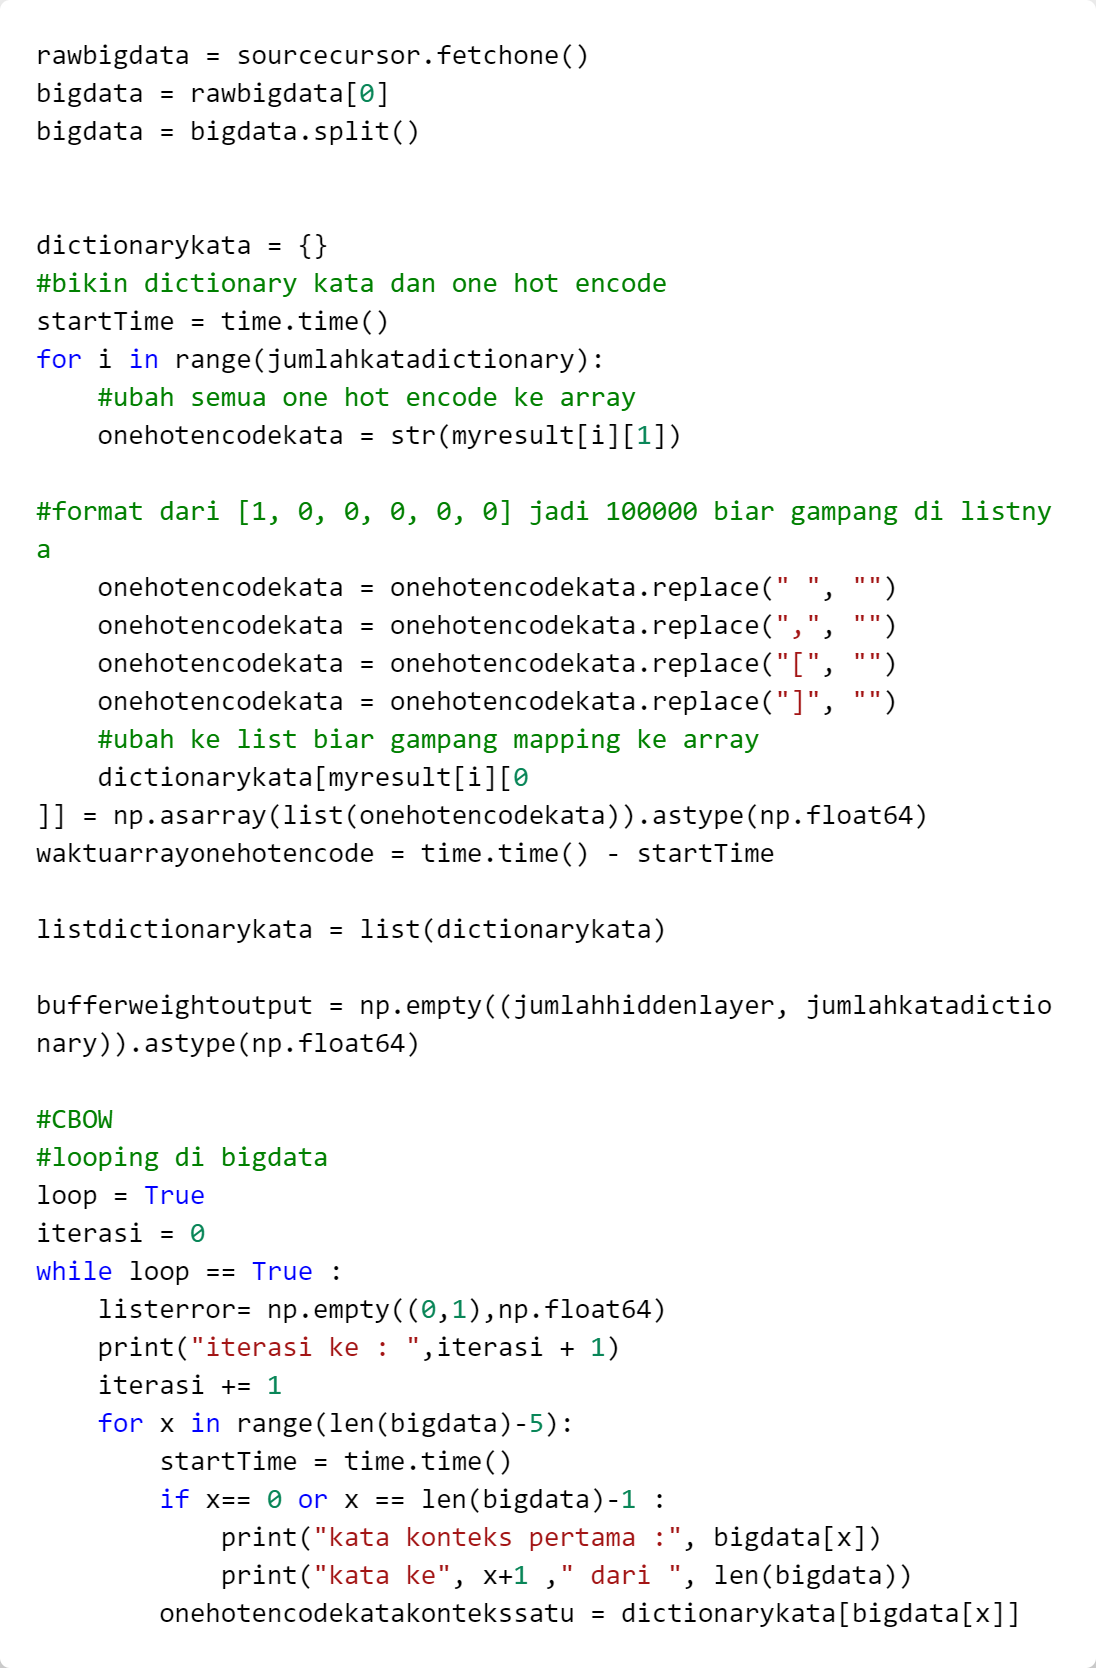
\includegraphics[scale=0.3]{trainingcbow4kata2}
\end{figure}
\begin{figure}[H]
\centering
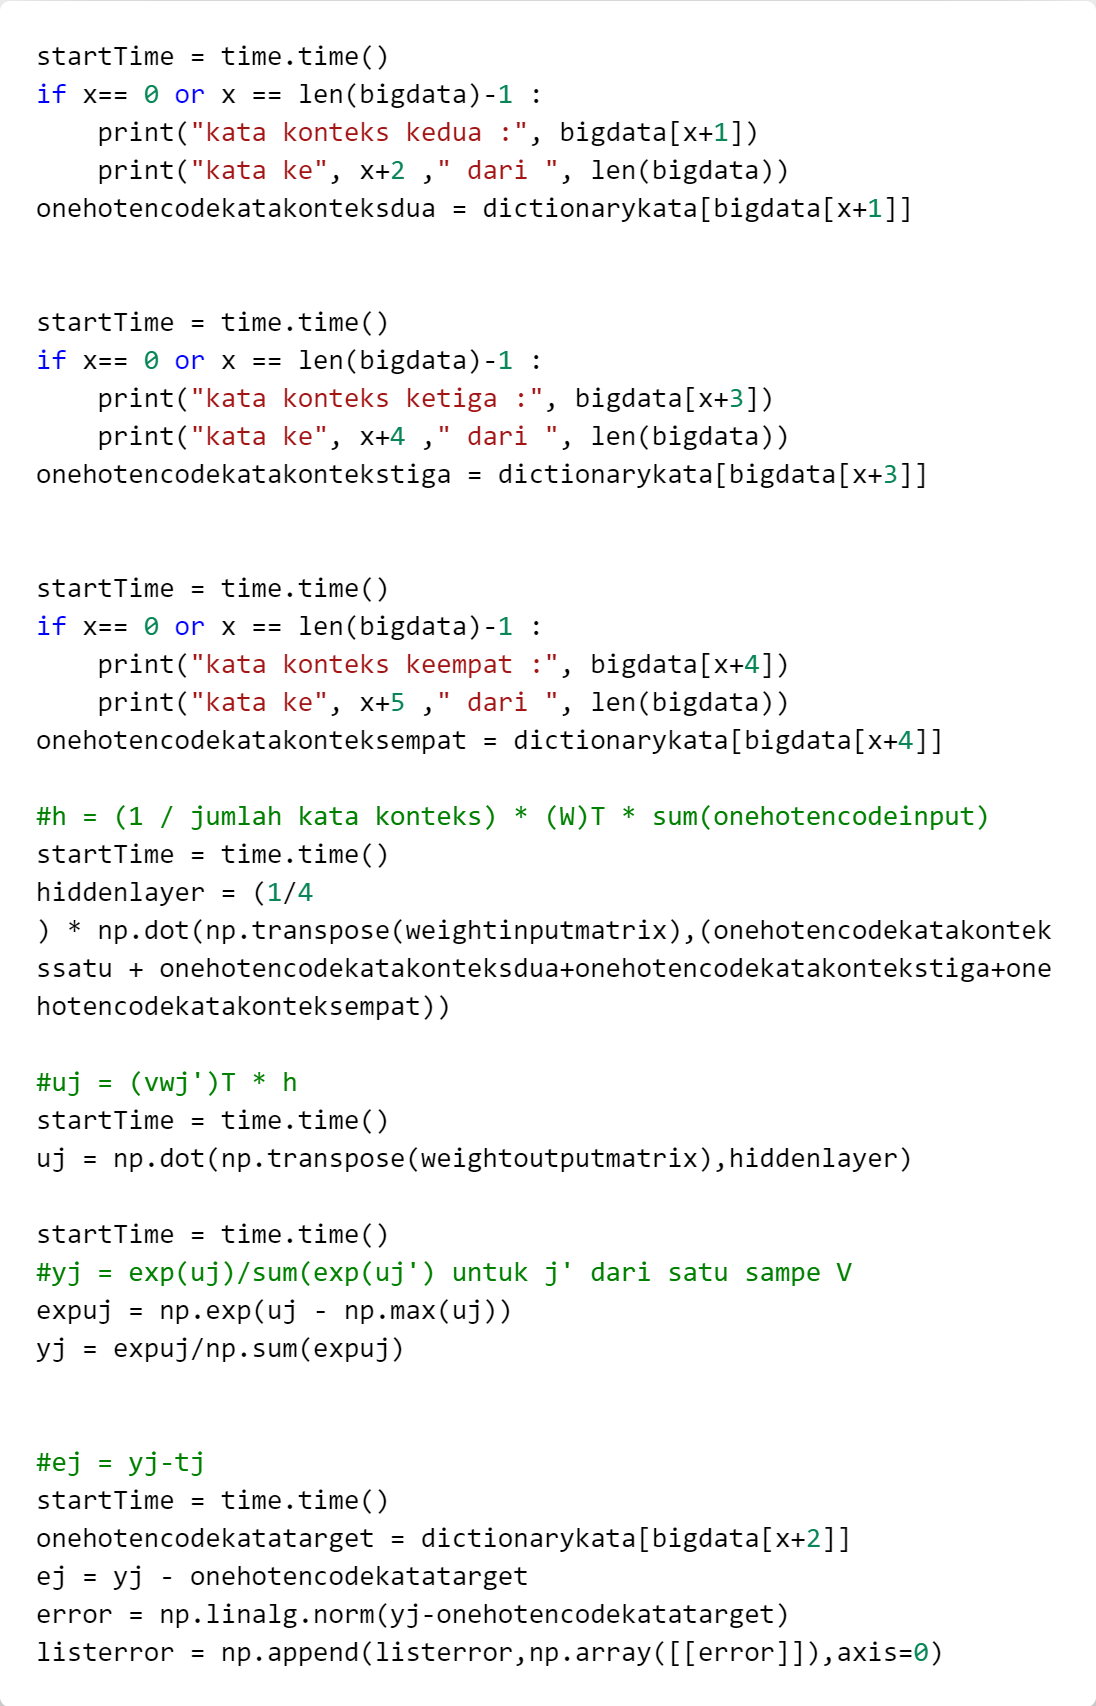
\includegraphics[scale=0.3]{trainingcbow4kata3}
\end{figure}
\begin{figure}[H]
\centering
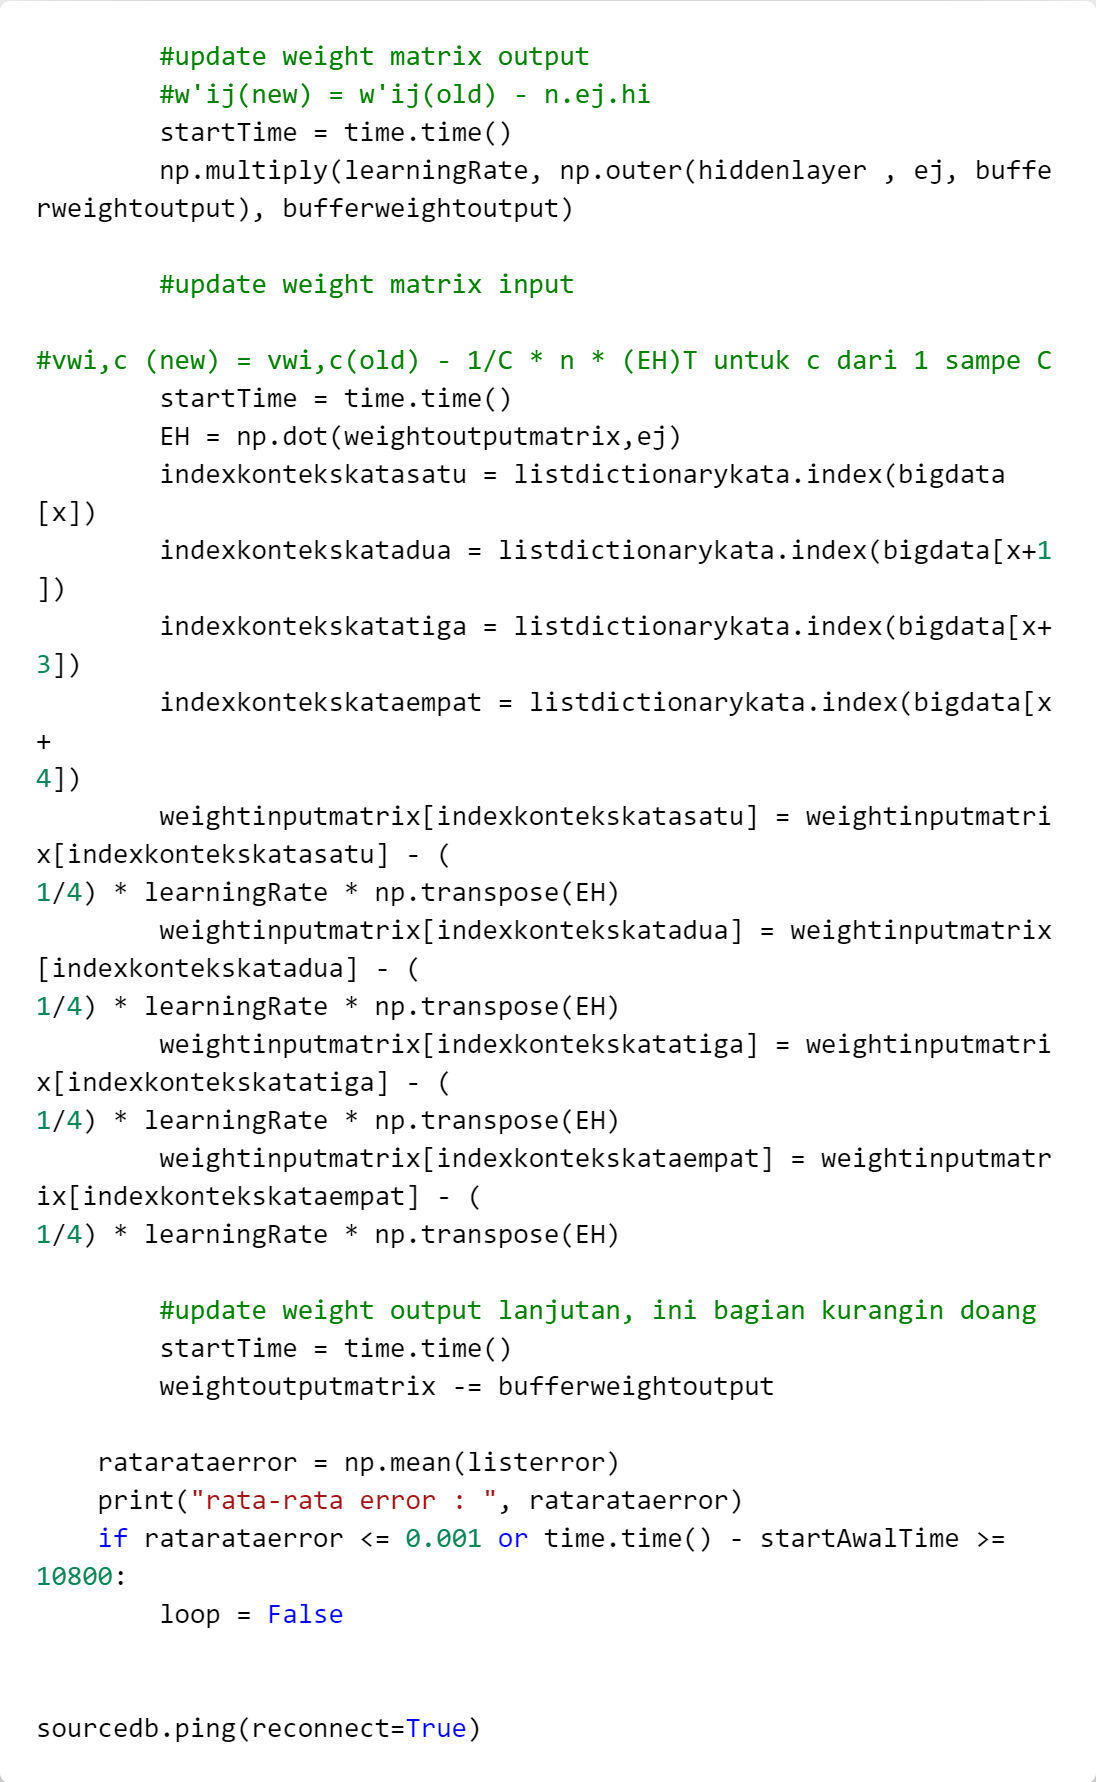
\includegraphics[scale=0.3]{trainingcbow4kata4}
\end{figure}
\begin{figure}[H]
\centering
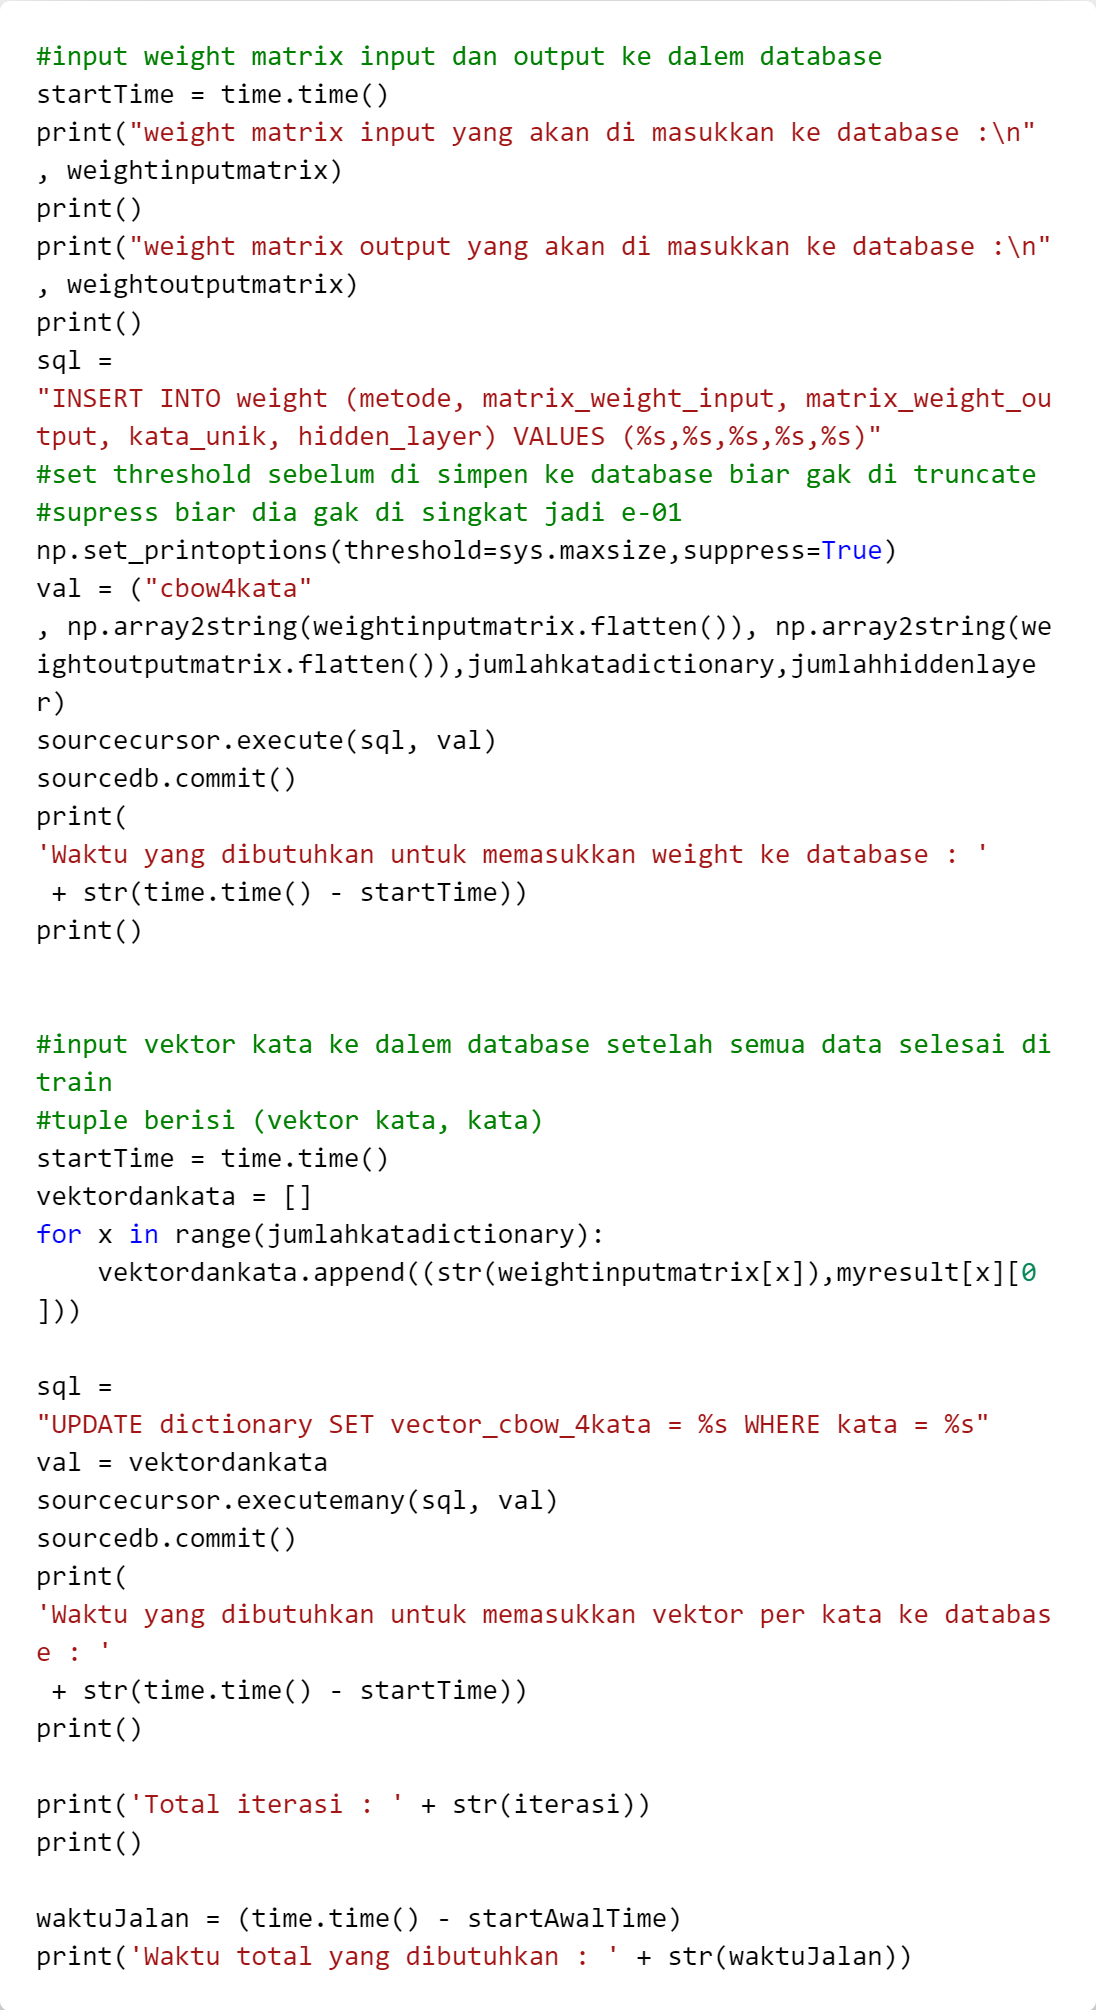
\includegraphics[scale=0.3]{trainingcbow4kata5}
\end{figure}

\newpage
{\parindent0pt \textbf{Lampiran 6 \textit{Source Code} search2cbow.py}}
\begin{figure}[H]
\centering
\includegraphics[scale=0.3]{search2cbow1}
\end{figure}
\begin{figure}[H]
\centering
\includegraphics[scale=0.3]{search2cbow2}
\end{figure}
\begin{figure}[H]
\centering
\includegraphics[scale=0.3]{search2cbow3}
\end{figure}
\begin{figure}[H]
\centering
\includegraphics[scale=0.3]{search2cbow4}
\end{figure}

\newpage
{\parindent0pt \textbf{Lampiran 7 \textit{Source Code} search4cbow.py}}
\begin{figure}[H]
\centering
\includegraphics[scale=0.3]{search4cbow1}
\end{figure}
\begin{figure}[H]
\centering
\includegraphics[scale=0.3]{search4cbow2}
\end{figure}
\begin{figure}[H]
\centering
\includegraphics[scale=0.3]{search4cbow3}
\end{figure}
\begin{figure}[H]
\centering
\includegraphics[scale=0.3]{search4cbow4}
\end{figure}

\newpage
\cleardoublepage
\phantomsection
\thispagestyle{plain}
\section*{RIWAYAT HIDUP}
\addcontentsline{toc}{section}{RIWAYAT HIDUP}

\textbf{MUHAMMAD ZALGHORNAIN}. Lahir di Jakarta, 19 Mei 1997, merupakan anak kedua dari pasangan Bapak Ir. Mochammad Nadjib Bachmid dan Ibu Wirdalita, S.Sos.

Penulis mengawali pendidikan di TK Islam Assalam II, Tambun, Bekasi pada tahun 2002-2003. Kemudian melanjutkan pendidikan di SD Jaya Suti Abadi, Tambun, Bekasi pada tahun 2003-2009. Selanjutnya penulis melanjutkan studi di SMPN 182, Pancoran, Jakarta Selatan pada tahun 2009-2012. Kemudian meneruskan ke SMAN 14, Jakarta Timur  pada tahun 2012-2015. Pada tahun 2015 penulis melanjutkan ke Universitas Negeri Jakarta (UNJ) melalui jalur SBMPTN. Di awal tahun 2023 (14 Februari 2023) penulis dinyatakan lulus dan mendapat gelar Sarjana Komputer (S.Kom), Program Studi Ilmu Komputer Fakultas Matematika dan Ilmu Pengetahuan Alam Universitas Negeri Jakarta.

\end{document}